\documentclass[11pt]{book}	%use"amsart"insteadof"article"forAMSLaTeXformat
\usepackage{geometry}		%Seegeometry.pdftolearnthelayoutoptions.Therearelots.
\geometry{letterpaper}		%...ora4paperora5paperor...
%\geometry{landscape}		%Activateforforrotatedpagegeometry
%\usepackage[parfill]{parskip}		%Activatetobeginparagraphswithanemptylineratherthananindent
\usepackage{graphicx}				%Usepdf,png,jpg,orepsßwithpdflatex;useepsinDVImode
								%TeXwillautomaticallyconverteps-->pdfinpdflatex		
\usepackage{amssymb}
\usepackage{amsmath}
\usepackage{amsthm}
\newtheorem{definition}{Definition}
\newtheorem{theorem}{Theorem}
\usepackage[colorlinks]{hyperref}

%----macros begin---------------------------------------------------------------
\usepackage{color}
\usepackage{amsthm}

\def\conv{\mbox{\textrm{conv}\,}}
\def\aff{\mbox{\textrm{aff}\,}}
\def\E{\mathbb{E}}
\def\R{\mathbb{R}}
\def\Z{\mathbb{Z}}
\def\tex{\TeX}
\def\latex{\LaTeX}
\def\v#1{{\bf #1}}
\def\p#1{{\bf #1}}
\def\T#1{{\bf #1}}

\def\vet#1{{\left(\begin{array}{cccccccccccccccccccc}#1\end{array}\right)}}
\def\mat#1{{\left(\begin{array}{cccccccccccccccccccc}#1\end{array}\right)}}

\def\lin{\mbox{\rm lin}\,}
\def\aff{\mbox{\rm aff}\,}
\def\pos{\mbox{\rm pos}\,}
\def\cone{\mbox{\rm cone}\,}
\def\conv{\mbox{\rm conv}\,}
\newcommand{\homog}[0]{\mbox{\rm homog}\,}
\newcommand{\relint}[0]{\mbox{\rm relint}\,}

%----macros end-----------------------------------------------------------------

\title{LARCC --- LINEAR ALGEBRAIC REPRESENTATION FOR COMPUTING WITH COCHAINS
%\footnote{This document is part of the \emph{Linear Algebraic Representation with CoChains} (LAR-CC) framework~\cite{cclar-proj:2013:00}. \today}
}
\author{LARCC Team}
\date{\today}							%Activatetodisplayagivendateornodate

\begin{document}
\maketitle
\nonstopmode

\tableofcontents
\newpage

\begin{document}


\documentclass[11pt,oneside]{article}	%use"amsart"insteadof"article"forAMSLaTeXformat
\usepackage{geometry}		%Seegeometry.pdftolearnthelayoutoptions.Therearelots.
\geometry{letterpaper}		%...ora4paperora5paperor...
%\geometry{landscape}		%Activateforforrotatedpagegeometry
%\usepackage[parfill]{parskip}		%Activatetobeginparagraphswithanemptylineratherthananindent
%\usepackage{graphicx}				%Usepdf,png,jpg,oreps§withpdflatex;useepsinDVImode
								%TeXwillautomaticallyconverteps-->pdfinpdflatex		
\usepackage{amssymb}
\usepackage[colorlinks=true]{hyperref}
\usepackage{qtree}

%----macros begin-----------------------------------------------------------------------------------
\usepackage{graphicx}
\usepackage{color}
\usepackage{amsthm}

%\renewenvironment{Shaded}{\pause\begin{snugshade}}{\end{snugshade}}
\def\twocolumns#1#2{\begin{columns}
\begin{column}{0.5\linewidth}#1\end{column}
\begin{column}{0.5\linewidth}#2\end{column}
\end{columns}}
\def\mytwocolumns#1#2#3#4{\begin{columns}
\begin{column}{#1\linewidth}#2\end{column}
\begin{column}{#3\linewidth}#4\end{column}
\end{columns}}
\def\mythreecolumns#1#2#3#4#5#6{\begin{columns}
\begin{column}{#1\linewidth}#2\end{column}
\begin{column}{#3\linewidth}#4\end{column}
\begin{column}{#5\linewidth}#6\end{column}
\end{columns}}
\def\threecolumns#1#2#3{\begin{columns}
\begin{column}{0.33\linewidth}#1\end{column}
\begin{column}{0.33\linewidth}#2\end{column}
\begin{column}{0.33\linewidth}#3\end{column}
\end{columns}}
\def\fourcolumns#1#2#3#4{\begin{columns}%
\begin{column}{0.25\linewidth}#1\end{column}%
\begin{column}{0.25\linewidth}#2\end{column}%
\begin{column}{0.25\linewidth}#3\end{column}%
\begin{column}{0.25\linewidth}#4\end{column}%
\end{columns}}

\def\conv{\mbox{\textrm{conv}\,}}
\def\aff{\mbox{\textrm{aff}\,}}
\def\E{\mathbb{E}}
\def\R{\mathbb{R}}
\def\Z{\mathbb{Z}}
\def\tex{\TeX}
\def\latex{\LaTeX}
\def\v#1{{\bf #1}}
\def\p#1{{\bf #1}}
\def\T#1{{\bf #1}}

\def\vet#1{{\left(\begin{array}{cccccccccccccccccccc}#1\end{array}\right)}}
\def\mat#1{{\left(\begin{array}{cccccccccccccccccccc}#1\end{array}\right)}}

\def\lin{\mbox{\rm lin}\,}
\def\aff{\mbox{\rm aff}\,}
\def\pos{\mbox{\rm pos}\,}
\def\cone{\mbox{\rm cone}\,}
\def\conv{\mbox{\rm conv}\,}
\newcommand{\homog}[0]{\mbox{\rm homog}\,}
\newcommand{\relint}[0]{\mbox{\rm relint}\,}

%----macros end-----------------------------------------------------------------------------------


\title{Literate programming IDE for LAR-CC 
\footnote{This document is part of the \emph{Linear Algebraic Representation with CoChains} (LAR-CC) framework~\cite{cclar-proj:2013:00}. \today}
}
\author{Alberto Paoluzzi}
%\date{}							%Activatetodisplayagivendateornodate

\begin{document}
\maketitle
%\nonstopmode

\begin{abstract}
This document introduces the developer of geometric libreries and applications to  the integrated development environment (IDE)  set up for documentation and multilanguage development  using LAR-CC, the Linear Algebraic Representation for geometry, manufacturing and physics with \emph{Chains} and \emph{CoChains}. This IDE is strongly based on the \href{http://www.literateprogramming.com/}{literate programming} tool \emph{Nuweb}, aiming at embedding the code in the documentation, and not vice-versa.
The main goal of this framework is to facilitate how to express the \emph{why} of software design decisions, and not only the tricky details of low level coding.  I would recommend writing programs as if they were research papers and treat the code as you would write mathematical expressions in a research paper. Using multiple programming languages is allowed and even encouraged in \texttt{larcc}. When possible, the same functions coded in different languages should stay close within the same document subsection. The \texttt{larcc} IDE integrates a few programming, documentation and version control tools, including \href{http://www.tug.org/texlive/}{\LaTeX}, \href{http://sourceforge.net/projects/nuweb/}{\emph{Nuweb}}, \href{http://johnmacfarlane.net/pandoc/}{\emph{Pandoc}},  \href{http://git-scm.com/}{\emph{Git}}, and \href{http://leoeditor.com/}{Leo editor}.
\end{abstract}

\tableofcontents
\section{Up and running}

\subsection{Prerequisites}

\paragraph{\LaTeX}
The \texttt{larcc} IDE requires the users to embed the compute code within \LaTeX\ files written for documenting their work. Therefore the first requirement is a working \LaTeX\ environment. ``As \TeX\ Live is the basis of Mac\TeX, and is the \TeX\ system for Unix, if you work cross-platform and want an identical system on all of your machines, then \TeX\ Live is the way to go''~\cite{miktek:2012}.

\paragraph{Python}
As of today, most of \texttt{larcc} development was done in Python. Hence a working Python environment is required, including three packages: \href{http://www.scipy.org}{\texttt{scipy}}, \href{http://pyopengl.sourceforge.net}{\texttt{pyopengl}}, and \href{https://github.com/plasm-language/pyplasm}{\texttt{pyplasm}}. On a Mac, Python is installed by default, whereas \texttt{scipy} and \texttt{pyopengl} may be installed in the terminal by doing 
\begin{verbatim}
$ sudo easy-install scipy
$ sudo easy-install pyopengl
\end{verbatim}
Finally, to install \texttt{pyplasm} look at the README file in its downloaded directory:
\begin{verbatim}
$ git clone https://github.com/plasm-language/pyplasm
\end{verbatim}

\paragraph{Nuweb}

In 1984, Knuth introduced the idea of literate programming. The idea was that a programmer writes just one document, the web file---with suffix \texttt{.w}, that combines the documentation with the code. \emph{Nuweb} works with any programming language and \LaTeX, and is probably the simplest incarnation of the Knut's original work.
The web site of the tool is \href{http://sourceforge.net/projects/nuweb/}{sourceforge.net/projects/nuweb/}.
A revised version of source files can be found on \href{https://code.google.com/p/nuweb/downloads/list}{code.google.com/p/nuweb}. This package can build using the standard tools:
\begin{verbatim}
$ cd <path-to>/nuweb/
$ ./configure
$ make
$ sudo make install
\end{verbatim}
For some documentation read the \href{https://code.google.com/p/nuweb/source/browse/branches/qse-nuweb/README?r=3}{wiki} page.  Test your installation by just compiling to \emph{pdf} the \texttt{nuweb.w} document itself, whose chapter one contains the user documentation:
\begin{verbatim}
$ nuweb nuweb.w
\end{verbatim}
Of course, in order to extend \texttt{larcc} and/or to make an efficient use of it, you are supposed to read carefully the first chapter of the \emph{nuweb.pdf} document.

\subsection{Download}

You may or may not put your IDE under the protection of a version control system. The \texttt{larcc} project comes from \emph{Github} equipped with an integrated \emph{git} system, that you are free either to use or not to use. Of course, my advice  is of making the best use of it. Hence write in the terminal:
\begin{verbatim}
$ git clone https://github.com/cvdlab/larcc
\end{verbatim}

Thats all. Now move to the \texttt{larcc} directory and give a look at its content, a bunch of directories, subdirectories and files, of course. Write
\begin{verbatim}
$ tree -L 2
\end{verbatim}
and you will see something like
\begin{figure}[htbp] %  figure placement: here, top, bottom, or page
   \centering
   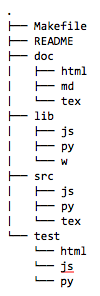
\includegraphics[width=2cm]{images/tree.png} 
   \caption{A sample of the \texttt{larcc} framework}
   \label{fig:tree}
\end{figure}

\subsection{Working-file}
For the impatient, open a terminal, and change directory to \texttt{larcc}, the root of the LAR-CC project, if not already there, whenever you hold it on your system. Then create your working-file \texttt{src/tex/<name>.tex} as a copy of \texttt{src/tex/template.tex}. Open the working-file with an editor, possibly with one aware of the \LaTeX\ syntax, and make few mandatory changes on the template text: 

\begin{description}
\item[Title] change the \texttt{title} command, substituting the ``Title'' string with the actual sentence to be used as document title;
\item[Author]  do the same for the \texttt{author} command, substituting the ``TheAuthor'' string with the actual document author;

\item[Bibliography] substitute the ``template'' string with the actual working-file name (without the file extension).
\end{description}

Finally you may starting the real work by writing the documentation/code within your \texttt{<name>.tex} file, using the simple mark-up rules of \href{run:nuwebdoc.pdf}{Nuweb}.

\subsection{Using the IDE}

In short, in order to use the development environment, you must (a) open your terminal and move to the \texttt{larcc} directory, (b) write a \texttt{tex} file, including documentation and suitably tagged computer code, (c) save it in the \texttt{src} subdirectory, and (d)  execute a \texttt{make} command, asking either for generation of the \texttt{pdf} or the \texttt{html} documentation, or  execution of \href{http://en.wikipedia.org/wiki/Unit_testing}{unit testing}, or simply for the compilation of the source code.


\subsubsection{Using Leo}

\href{http://leoeditor.com}{Leo} is a multi-platform and open-source outliner and \emph{non-linear} text editor allowing for 
fundamentally different ways of using and organizing data, programs and scripts. 
Leo has been under active development for 15 years and has an active group of developers and users.
The Leo environment allow to structure either simple or very complex projects as an acyclic graph, where nodes (said clones), and hence the subgraphs rooted in them, may have more than one father.
Accordingly, every update to a clone node immediately extends to every its instances within the tree-like walk-through of the whole outline.


\subsubsection{Using make}

When using the IDE, the user must open the \texttt{Makefile} with any text editor, and modify the current values of two user-definable variables, according to his will:

\begin{verbatim}
NAME = <name>
LANGUAGE = <language>
\end{verbatim}
where \texttt{<name>} is name of the new working document, and \texttt{<language>} may be only \texttt{py} (for Pyton). Soon such values will be extended to include \texttt{<js>} for Javascript and \texttt{<lhs>} for Literate Haskell.
The make \emph{targets} currently available in the Makefile are the following:
\begin{description}
\item[all] 
is the default option. Its execution produces a \emph{pdf} document in the \texttt{doc/pdf} subdirectory, and a pair of \emph{tex}/\emph{bbl} documents in the \texttt{doc/tex} subdirectory, all using name \texttt{<name>};
\item[html] 
similar to the default option, but produces a directory named \texttt{<name>} wth a bunch of \emph{html} pages, located in the \texttt{doc/html} subdirectory;

\item[test] 
to execute the tests contained in the directory \texttt{test/<language>/<name>}
\item[exec] 
to execute \emph{nuweb} on the working document, i.e.~on \texttt{<name>.tex}\footnote{Actually, \texttt{<name>.tex} is internally copied to a scratch file \texttt{<name>.w}, in order to allow the user to work comfortably with an editor knowledgeable of the \LaTeX\ syntax.}; this execution generates both the \LaTeX\ documentation file and the source output files (for example the unit tests) written in the coding \texttt{<language>};
\item[clear] 
to remove all the working files from the root directory. Used by other commands. To be invoked by the user just in case that something did not work out.
\end{description}



\section{Structure of \texttt{larcc}}

The \texttt{larcc} project is hinged around four subdirectories (see Figure~\ref{fig:tree}) and a Makefile.
The meaning and function of the four subdirectories are listed below.

\begin{description}
\item[src]  (for \emph{Source})
is the directory \texttt{src}  that contains all the source documents, and in particular the \texttt{tex} files including the code of the algorithms and the tests developed in the project. It is divided in subdirectories related to the type of the source file itself. For example a \texttt{html} directory will contain the user-defined \texttt{css} source files, and the \texttt{lhs} directory the \emph{literate Haskell} sorce files, to be processed directly by the Haskell compiler \emph{GHC}.
Such directories will also contain other programming resources needed to build the libreries or the applications developed in the LAR-CC project.

\item[test] 
\href{http://en.wikipedia.org/wiki/Test-driven_development}{test-driven development} (TDD) is a software development process that relies on the repetition of a very short development cycle: write a ``unit test'', get it to pass, run all tests, clean up the code (see Figure~\ref{fig:tdd}).
The subdirectory \texttt{test} is the repository of test suites, collection of test cases, and of unit test files, possibly grouped depending on the source language, to be launched either individually, while writing each single software function or application, or collectively before committing or pushing novel developments or subsystems. 

\item[lib] 
is the repository of compiled and/or executable programs. In particular, it is the place where to store and retrieve all the libreries or modules or applications developed by compilation of any  document within the \texttt{scr} subdirectory of the \texttt{larcc} system, excluding the documentation.

\item[doc] 
conversely contains all the documentation generated by the system, once again subdivided depending on the language and tools used for its reading or examination.
\end{description}

\begin{figure}[htbp] %  figure placement: here, top, bottom, or page
   \centering
   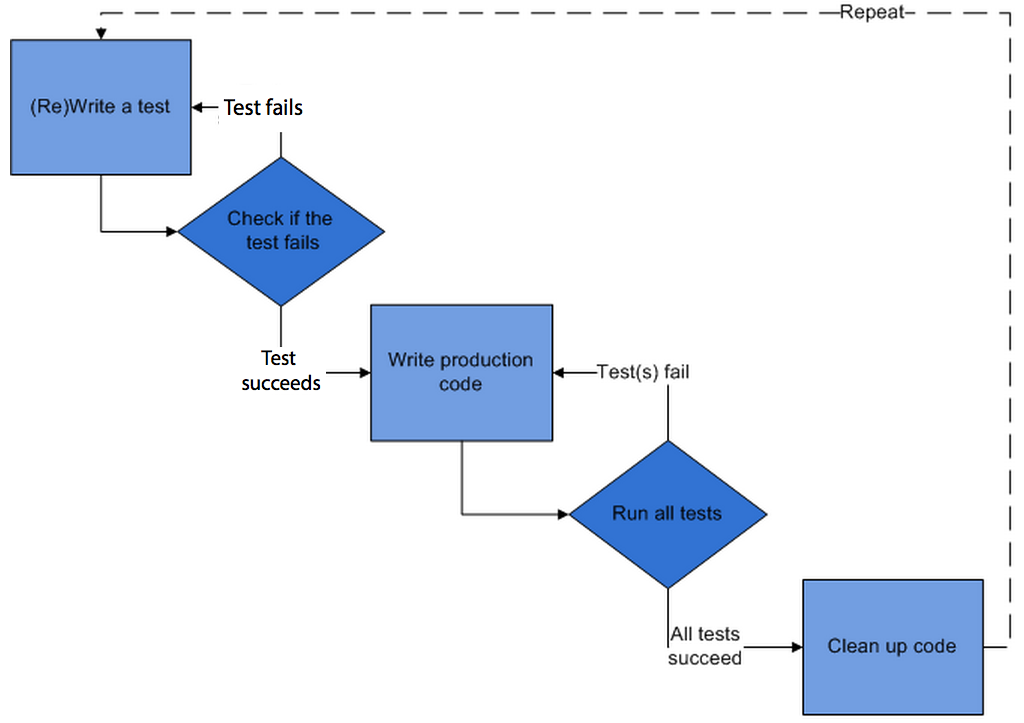
\includegraphics[width=0.8\linewidth]{images/tdd.png} 
   \caption{test-driven development (TDD) cycle (from Wikipedia)}
   \label{fig:tdd}
\end{figure}

\bibliographystyle{amsalpha}
\bibliography{frame}

\end{document}


\documentclass[11pt,oneside]{article}	%use"amsart"insteadof"article"forAMSLaTeXformat
\usepackage{geometry}		%Seegeometry.pdftolearnthelayoutoptions.Therearelots.
\geometry{letterpaper}		%...ora4paperora5paperor...
%\geometry{landscape}		%Activateforforrotatedpagegeometry
%\usepackage[parfill]{parskip}		%Activatetobeginparagraphswithanemptylineratherthananindent
\usepackage{graphicx}				%Usepdf,png,jpg,orepsßwithpdflatex;useepsinDVImode
								%TeXwillautomaticallyconverteps-->pdfinpdflatex		
\usepackage{amssymb,amsmath,amsthm}
\newtheorem{definition}{Definition}
\usepackage[colorlinks=true]{hyperref}

%----macros begin-----------------------------------------------------------------------------------
\usepackage{graphicx}
\usepackage{color}
\usepackage{amsthm}

%\renewenvironment{Shaded}{\pause\begin{snugshade}}{\end{snugshade}}
\def\twocolumns#1#2{\begin{columns}
\begin{column}{0.5\linewidth}#1\end{column}
\begin{column}{0.5\linewidth}#2\end{column}
\end{columns}}
\def\mytwocolumns#1#2#3#4{\begin{columns}
\begin{column}{#1\linewidth}#2\end{column}
\begin{column}{#3\linewidth}#4\end{column}
\end{columns}}
\def\mythreecolumns#1#2#3#4#5#6{\begin{columns}
\begin{column}{#1\linewidth}#2\end{column}
\begin{column}{#3\linewidth}#4\end{column}
\begin{column}{#5\linewidth}#6\end{column}
\end{columns}}
\def\threecolumns#1#2#3{\begin{columns}
\begin{column}{0.33\linewidth}#1\end{column}
\begin{column}{0.33\linewidth}#2\end{column}
\begin{column}{0.33\linewidth}#3\end{column}
\end{columns}}
\def\fourcolumns#1#2#3#4{\begin{columns}%
\begin{column}{0.25\linewidth}#1\end{column}%
\begin{column}{0.25\linewidth}#2\end{column}%
\begin{column}{0.25\linewidth}#3\end{column}%
\begin{column}{0.25\linewidth}#4\end{column}%
\end{columns}}

\def\conv{\mbox{\textrm{conv}\,}}
\def\aff{\mbox{\textrm{aff}\,}}
\def\E{\mathbb{E}}
\def\R{\mathbb{R}}
\def\Z{\mathbb{Z}}
\def\tex{\TeX}
\def\latex{\LaTeX}
\def\v#1{{\bf #1}}
\def\p#1{{\bf #1}}
\def\T#1{{\bf #1}}

\def\vet#1{{\left(\begin{array}{cccccccccccccccccccc}#1\end{array}\right)}}
\def\mat#1{{\left(\begin{array}{cccccccccccccccccccc}#1\end{array}\right)}}

\def\lin{\mbox{\rm lin}\,}
\def\aff{\mbox{\rm aff}\,}
\def\pos{\mbox{\rm pos}\,}
\def\cone{\mbox{\rm cone}\,}
\def\conv{\mbox{\rm conv}\,}
\newcommand{\homog}[0]{\mbox{\rm homog}\,}
\newcommand{\relint}[0]{\mbox{\rm relint}\,}

%----macros end-----------------------------------------------------------------------------------


\title{Module Lar2psm
\footnote{This document is part of the \emph{Linear Algebraic Representation with CoChains} (LAR-CC) framework~\cite{cclar-proj:2013:00}. \today}
}
\author{Alberto Paoluzzi}
%\date{}							%Activatetodisplayagivendateornodate

\begin{document}
\maketitle
%\nonstopmode

\begin{abstract}
This software module contains all the functions needed to interface the LAR data structure and/or the geometric  objects defined by it with the Plasm environment. In particular, it will include the interfaces towards the visualization primitives provided by the language.
\end{abstract}



\tableofcontents
\newpage

\section{Introduction}
The standard definition of vectors and matrices in plasm is the list of vector coordinates and the list of matrix rows, respectively.

\section{Implementation}

Since the present \texttt{lar2psm} module is an interface between the \texttt{larcc} library and the PLaSM language, and its various incarnations, it should allow to import the language itself (in Python, the \texttt{pyplasm} module). 
%------------------------------------------------------------------
@d Import the pyplasm module
@{from pyplasm import * 
@}
%------------------------------------------------------------------

An useful utility will allow for the creation of a subdirectory from a \texttt{dirpath} \emph{string}.
%------------------------------------------------------------------
@d Create directory from path 
@{import os
def createDir(dirpath):
    if not os.path.exists(dirpath):
        os.makedirs(dirpath)
@| createDir @}
%------------------------------------------------------------------

It may be useful to define the repository(ies) for the unit tests associated to the module:
%------------------------------------------------------------------
@o test/py/lar2psm-tests.py
@{@< Create directory from path @>
createDir('test/py/lar2psm/')
@}
%------------------------------------------------------------------


\subsection{Convex combination}
Next we define the \texttt{CCOMB} function that accepts as input a \texttt{vectors} list (i.e., a matrix) and returns \emph{the} point their convex combination.
%------------------------------------------------------------------
@d Compute the convex combination of a list of vectors
@{import scipy as sp
from pyplasm import *
def CCOMB(vectors):
    return (sp.array(VECTSUM(vectors)) / float(len(vectors))).tolist()  
@| CCOMB @}
%------------------------------------------------------------------

\paragraph{Unit tests}
First we test \texttt{CCOMB} with some special data, then with some random vectors.
%------------------------------------------------------------------
@o test/py/lar2psm/test-ccomb.py
@{@< Import the module @(lar2psm@) @>
from lar2psm import *
@< \texttt{CCOMB} unit tests @>
@}
%------------------------------------------------------------------

\subsection{LAR model of a cell complex}

A very important concept introduced by the LAR package is the definition of the \emph{model} of a cell complex, as a pair made by a list of vertices, given as lists of coordinates, and a topological relation.

\begin{definition}[LAR model]
A \emph{LAR model} is a pair, e.g.~a Python tuple \emph{\texttt(V, FV)}, where:
\begin{enumerate}
\item \texttt{V} is the list of vertices, given as lists of coordinates;
\item \texttt{FV} is a \emph{cell-vertex} relation, in this case the face-vertex relation, given as a list of cells, where each cell is given as a list of vertex indices.
\end{enumerate}
\end{definition}

\paragraph{Examples} 
Some very simple examples of 0D, 1D, and 2D models follows. They are displayed in Figure~\ref{fig:lar2psm-01}.
%------------------------------------------------------------------
@d 2D model examples 
@{V = [[0.,0.],[1.,0.],[0.,1.],[1.,1.],[0.5,0.5]]
VV = [[0],[1],[2],[3],[4]]
EV = [[0,1],[0,2],[0,4],[1,3],[1,4],[2,3],[2,4],[3,4]]
FV = [[0,1,4],[1,3,4],[2,3,4],[0,2,4]]

model0d, model1d, model2d = (V,VV), (V,EV), (V,FV)
@}
%------------------------------------------------------------------

\subsection{Function \texttt{MKPOLS}}

The function \texttt{MKPOLS} returns a list of HPC objects, i.e.~the geometric type of the PLaSM language. This list is generated to be displayed, possibly exploded, by the \texttt{pyplasm} viewer. 

Each cell \texttt{f} in the model (i.e.~each vertex list in the \texttt{FV} array of the previous example) is mapped into a polyhedral cell by the \texttt{pyplasm} operator \texttt{MKPOL}. The vertex indices are mapped from base 0 (the Python and C standard) to base 1 (the Plasm, Matlab, and FORTRAN standard).
%------------------------------------------------------------------
@d MaKe a list of HPC objects from a LAR model
@{def MKPOLS (model):
    V, FV = model
    pols = [MKPOL([[V[v] for v in f],[range(1,len(f)+1)], None]) for f in FV]
    return pols  
@| MKPOLS @}
%------------------------------------------------------------------

\paragraph{Unit tests}
Some simple 3D, 2D, 1D and 0D models are generated and visualised exploded by the file
%------------------------------------------------------------------
@o test/py/lar2psm/test-models.py
@{@< Import the module @(lar2psm@) @>
@< View model examples @>
@}
%------------------------------------------------------------------

\subsection{``Explosion'' of the scene}

A function \texttt{EXPLODE} used to ``explode'' an HPC scene defined as a \emph{list} of HPC values, given three real scaling parameters, \texttt{sx,sy,sz}, that are used to transform the position of the centroid of each HPC cell. HPC stands for \emph{HierarchicaL Polyhedral Complex}, the  type of plasm geometric values. Of course the assertion
\[
sx,sy,sz \geq 1.0
\]
must be true, otherways the function would induce some compenetration of the cells of the scene.

%------------------------------------------------------------------
@d Explode the scene using \texttt{sx,sy,sz} scaling parameters
@{def EXPLODE (sx,sy,sz):
    def explode0 (scene):
        centers = [CCOMB(S1(UKPOL(obj))) for obj in scene]
        scalings = len(centers) * [S([1,2,3])([sx,sy,sz])]
        scaledCenters = [UK(APPLY(pair)) for pair in
                         zip(scalings, [MK(p) for p in centers])]
        translVectors = [ VECTDIFF((p,q)) for (p,q) in zip(scaledCenters, centers) ]
        translations = [ T([1,2,3])(v) for v in translVectors ]
        return STRUCT([ t(obj) for (t,obj) in zip(translations,scene) ])
    return explode0  
@| EXPLODE @}
%------------------------------------------------------------------

The \texttt{EXPLODE} function is second order: it first application (to the scaling parameters) returns a partial function to be applied to the \texttt{scene}, given as a \emph{list} of HPC (Hierarchical Polyhedral Complex) objects. 
\texttt{EXPLODE} is dimension-independent, since it can be applied to points, edges, faces, 3D cells, and even to geometric values of mixed dimensionality (see Figure~\ref{fig:lar2psm-01}).

It works by computing the centroid of each object, and by applying to each of them a translation equal to the difference betwwen the scaled and the initial positions of its centroid. 
\texttt{EXPLODE}  returns a single HPC object (the assembly of input objects, properly translated)

\section{Source Output: \texttt{lar2psm} module}


\subsection{Importing a generic module}
First we define a parametric macro to allow the importing of \texttt{larcc} modules from the project repository \texttt{lib/py/}. When the user needs to import some project's module, she may call this macro as done in Section~\ref{sec:lar2psm}.
%------------------------------------------------------------------
@d Import the module
@{import sys
sys.path.insert(0, 'lib/py/')
import @1
@}
%------------------------------------------------------------------

\paragraph{Importing a module} A function used to import a generic \texttt{lacccc} module within the current environment is also useful.
%------------------------------------------------------------------
@d Function to import a generic module
@{def importModule(moduleName):
	@< Import the module @(moduleName@) @>
@| importModule @}
%------------------------------------------------------------------




\subsection{Lar2psm exporting}
\label{sec:lar2psm}
Here we assemble top-down the \texttt{lar2psm} module, by orderly listing the functional parts it is composed of. Of course, this one is the module version corresponding to the current state of the system, i.e.~to a very initial state. Other functions will be added when needed.
%------------------------------------------------------------------
@O lib/py/lar2psm.py
@{"""Module with functions needed to interface LAR with pyplasm"""
@< Import the module @(simplexn@) @>
@< Function to import a generic module @>
@< Compute the convex combination of a list of vectors @>
@< MaKe a list of HPC objects from a LAR model @>
@< Explode the scene using \texttt{sx,sy,sz} scaling parameters @>
@}
%------------------------------------------------------------------


\section{Unit tests}

\subsection{Creation of repository of unit tests}

A possible unit test strategy is to create a directory for unit tests associated to each source file in \texttt{nuweb}. Therefore we create here a directory in \texttt{test/py/} with the same name of the present document. Of course other 

%------------------------------------------------------------------
@d create directory and echo of creation
@{@< Create directory from path @>
@%i lib/py/lar2psm
createDir('@1')
print "'@1' repository created"
@}
%------------------------------------------------------------------

%------------------------------------------------------------------
@o test/py/lar2psm/test01.py
@{@< create directory  and echo of creation: @(test/py/lar2psm/@) @>
@}
%------------------------------------------------------------------


\subsection{Viewing some simplicial complexes}
Let we start producing some images, displayed in Figure~\ref{fig:lar2psm-01}, os a small simplicial complex and of its skeletons. Notice that the \texttt{+} character operates the join of lists (of HPC values).

%------------------------------------------------------------------
@d View model examples
@{from lar2psm import *
@< 2D model examples @>
explode = EXPLODE(1.5,1.5,1.5)
VIEW(explode(MKPOLS(model0d)))
VIEW(explode(MKPOLS(model1d)))
VIEW(explode(MKPOLS(model2d)))
VIEW(explode(MKPOLS(model2d) + MKPOLS(model1d) + MKPOLS(model0d)))
@}
%------------------------------------------------------------------


\begin{figure}[htbp] %  figure placement: here, top, bottom, or page
   \centering
   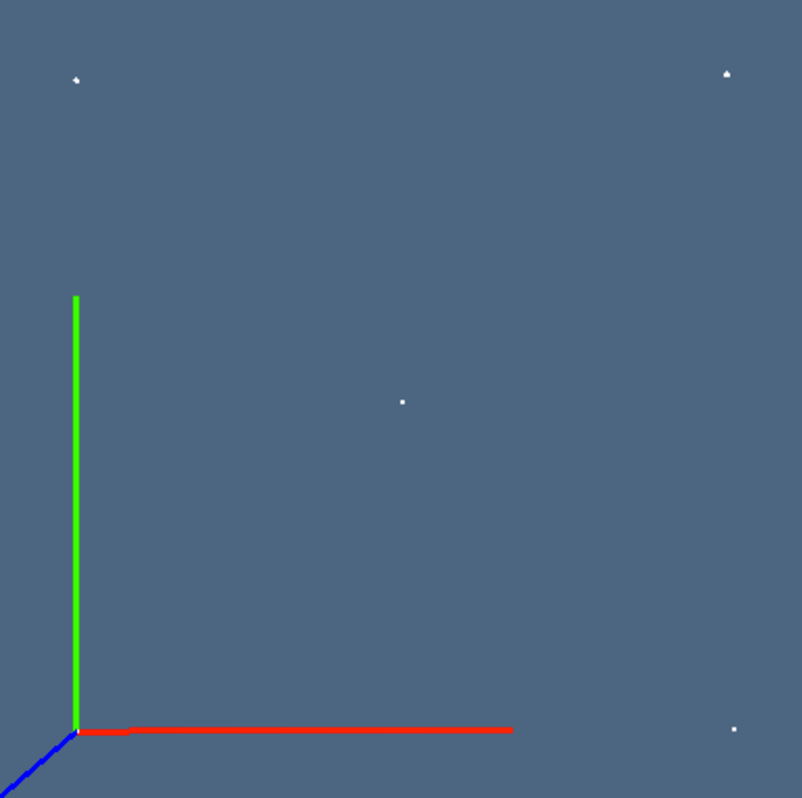
\includegraphics[height=0.245\linewidth,width=0.2425\linewidth]{images/lar2psm-01} 
   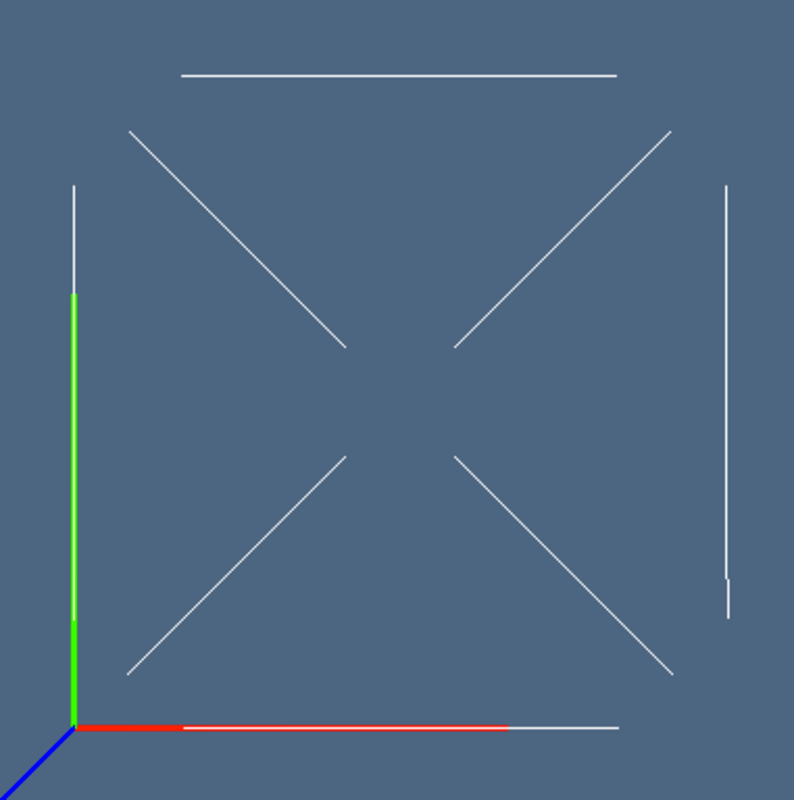
\includegraphics[height=0.245\linewidth,width=0.2425\linewidth]{images/lar2psm-02} 
   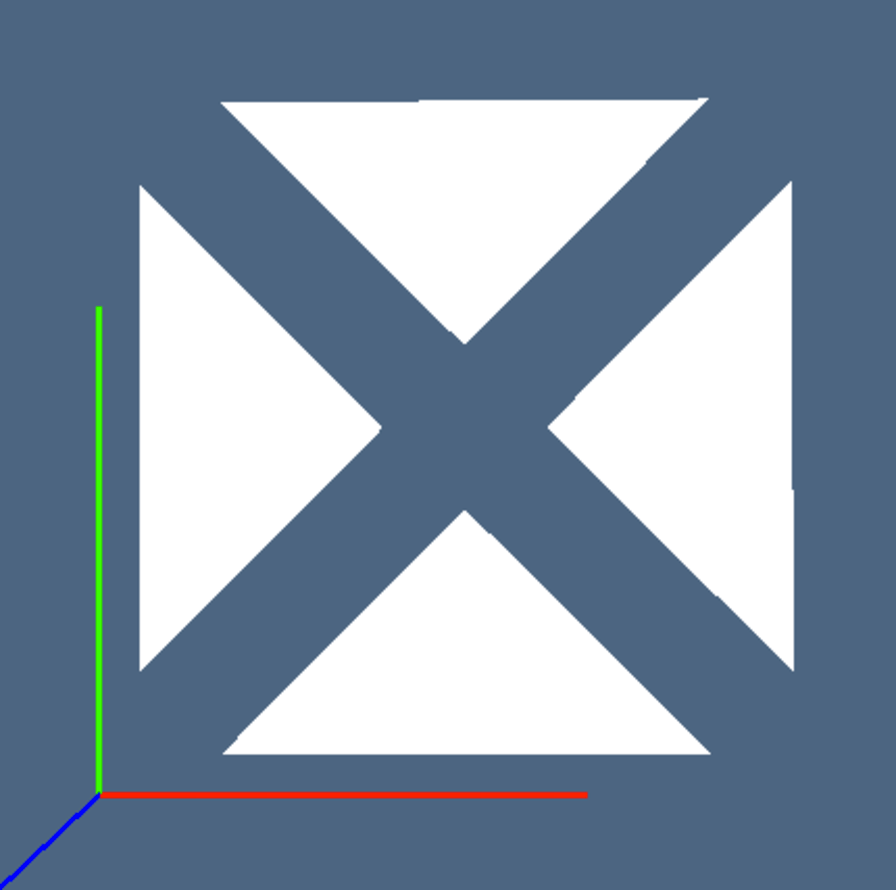
\includegraphics[height=0.245\linewidth,width=0.2425\linewidth]{images/lar2psm-03} 
   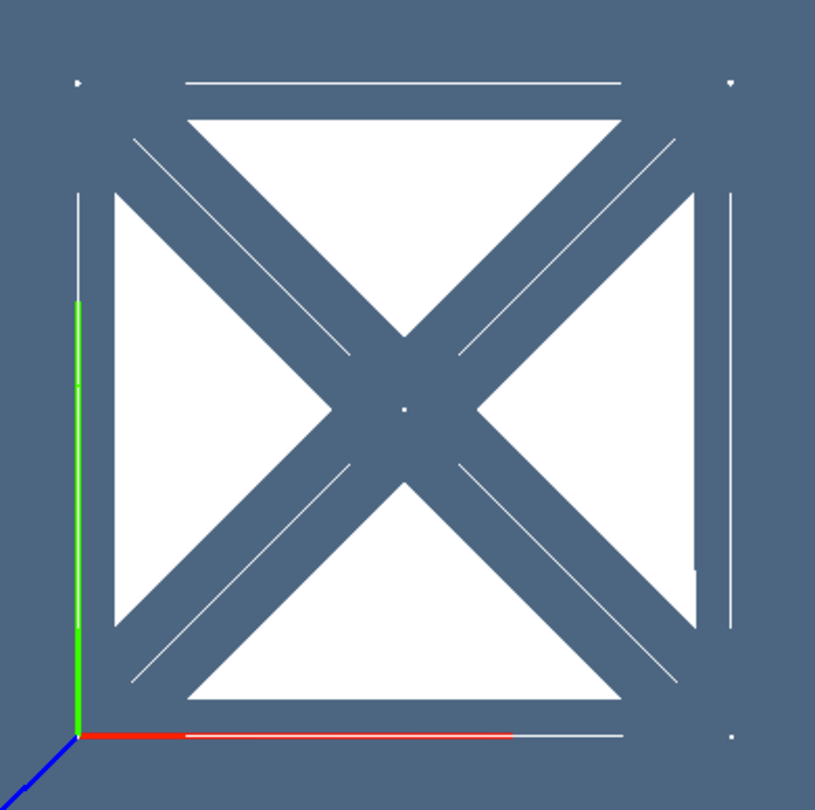
\includegraphics[height=0.245\linewidth,width=0.2425\linewidth]{images/lar2psm-04} 
   \caption{Images of the skeletons of a small simplicial complex.}
   \label{fig:lar2psm-01}
\end{figure}

\subsection{Testing convex combination of vectors}

%------------------------------------------------------------------
@d \texttt{CCOMB} unit tests
@{assert( CCOMB([]) == [] )
assert( CCOMB([[0,1]]) == [0.0, 1.0] )
assert( CCOMB([[0,1],[1,0]]) == [0.5, 0.5] )
assert( CCOMB([[1,0,0],[0,1,0],[0,0,1]]) == [1./3,1./3,1./3])

import random
vects = [[random.random() for i in range(3)] for k in range(4)]
assert( CCOMB([VECTSUM(vects)]) == \
        (sp.array(CCOMB(vects)) * len(vects)).tolist() )
@}
%------------------------------------------------------------------

\bibliographystyle{amsalpha}
\bibliography{lar2psm}

\end{document}

% -------------------------------------------------------------------------
% ------ nuweb macros (redefine as desired, or omit with "nuweb -p") ------
% -------------------------------------------------------------------------
\providecommand{\NWtxtMacroDefBy}{Macro defined by}
\providecommand{\NWtxtMacroRefIn}{Macro referenced in}
\providecommand{\NWtxtMacroNoRef}{Macro never referenced}
\providecommand{\NWtxtDefBy}{Defined by}
\providecommand{\NWtxtRefIn}{Referenced in}
\providecommand{\NWtxtNoRef}{Not referenced}
\providecommand{\NWtxtFileDefBy}{File defined by}
\providecommand{\NWsep}{${\diamond}$}
\providecommand{\NWlink}[2]{\hyperlink{#1}{#2}}
\providecommand{\NWtarget}[2]{% move baseline up by \baselineskip 
  \raisebox{\baselineskip}[1.5ex][0ex]{%
    \mbox{%
      \hypertarget{#1}{%
        \raisebox{-1\baselineskip}[0ex][0ex]{%
          \mbox{#2}%
}}}}}
% -------------------------------------------------------------------------

\documentclass[11pt,oneside]{article}	%use"amsart"insteadof"article"forAMSLaTeXformat
\usepackage{geometry}		%Seegeometry.pdftolearnthelayoutoptions.Therearelots.
\geometry{letterpaper}		%...ora4paperora5paperor...
%\geometry{landscape}		%Activateforforrotatedpagegeometry
%\usepackage[parfill]{parskip}		%Activatetobeginparagraphswithanemptylineratherthananindent
\usepackage{graphicx}				%Usepdf,png,jpg,orepsßwithpdflatex;useepsinDVImode
								%TeXwillautomaticallyconverteps-->pdfinpdflatex		
\usepackage{amssymb}
\usepackage{amsmath}
\usepackage{amsthm}
\newtheorem{definition}{Definition}
\newtheorem{theorem}{Theorem}

\usepackage[colorlinks]{hyperref}

%----macros begin-----------------------------------------------------------------------------------
\usepackage{graphicx}
\usepackage{color}
\usepackage{amsthm}

%\renewenvironment{Shaded}{\pause\begin{snugshade}}{\end{snugshade}}
\def\twocolumns#1#2{\begin{columns}
\begin{column}{0.5\linewidth}#1\end{column}
\begin{column}{0.5\linewidth}#2\end{column}
\end{columns}}
\def\mytwocolumns#1#2#3#4{\begin{columns}
\begin{column}{#1\linewidth}#2\end{column}
\begin{column}{#3\linewidth}#4\end{column}
\end{columns}}
\def\mythreecolumns#1#2#3#4#5#6{\begin{columns}
\begin{column}{#1\linewidth}#2\end{column}
\begin{column}{#3\linewidth}#4\end{column}
\begin{column}{#5\linewidth}#6\end{column}
\end{columns}}
\def\threecolumns#1#2#3{\begin{columns}
\begin{column}{0.33\linewidth}#1\end{column}
\begin{column}{0.33\linewidth}#2\end{column}
\begin{column}{0.33\linewidth}#3\end{column}
\end{columns}}
\def\fourcolumns#1#2#3#4{\begin{columns}%
\begin{column}{0.25\linewidth}#1\end{column}%
\begin{column}{0.25\linewidth}#2\end{column}%
\begin{column}{0.25\linewidth}#3\end{column}%
\begin{column}{0.25\linewidth}#4\end{column}%
\end{columns}}

\def\conv{\mbox{\textrm{conv}\,}}
\def\aff{\mbox{\textrm{aff}\,}}
\def\E{\mathbb{E}}
\def\R{\mathbb{R}}
\def\Z{\mathbb{Z}}
\def\tex{\TeX}
\def\latex{\LaTeX}
\def\v#1{{\bf #1}}
\def\p#1{{\bf #1}}
\def\T#1{{\bf #1}}

\def\vet#1{{\left(\begin{array}{cccccccccccccccccccc}#1\end{array}\right)}}
\def\mat#1{{\left(\begin{array}{cccccccccccccccccccc}#1\end{array}\right)}}

\def\lin{\mbox{\rm lin}\,}
\def\aff{\mbox{\rm aff}\,}
\def\pos{\mbox{\rm pos}\,}
\def\cone{\mbox{\rm cone}\,}
\def\conv{\mbox{\rm conv}\,}
\newcommand{\homog}[0]{\mbox{\rm homog}\,}
\newcommand{\relint}[0]{\mbox{\rm relint}\,}

%----macros end-----------------------------------------------------------------------------------


\title{The \texttt{smplxn} module
\footnote{This document is part of the framework~\cite{cclar-proj:2013:00}. \today}
}
\author{Alberto Paoluzzi}
%\date{}							%Activatetodisplayagivendateornodate

\begin{document}
\maketitle
\nonstopmode

\begin{abstract}
This module defines a minimal set of functions to generate a dimension-independent grid of simplices.
The name of the library was firstly used by our CAD Lab at University of Rome ``La Sapienza'' in years 1987/88 when we started working with dimension-independent simplicial complexes~\cite{Paoluzzi:1993:DMS:169728.169719}. This one in turn imports some functions from the \texttt{scipy} package and the geometric library \texttt{pyplasm}~\cite{}.
\end{abstract}

\tableofcontents\newpage

\section{Introduction}

The $Simple_X^n$ library, named \texttt{simplexn} within the Python version of the LARCC framework,
provides  combinatorial algorithms for some basic functions of geometric modelling with simplicial complexes. In particular, provides the efficient creation of simplicial complexes generated by simplicial complexes of lower dimension, the production of simplicial grids of any dimension, and the extraction of facets (i.e.~of $(d-1)$-faces) of complexes of $d$-simplices.

\section{Some simplicial algorithms}

The main aim of the simplicial functions given in this library is to provide optimal combinatorial algorithms, whose time complexity is linear in the size of the output.
Such a goal is achieved by calculating each cell in the output via closed combinatorial formulas, that do not require any searching nor data structure traversal to produce their results.

\subsection{Linear extrusion of a complex}

Here we discuss an implementation of the linear extrusion of simplicial complexes according to the method discussed in~\cite{Paoluzzi:1993:DMS:169728.169719} and~\cite{DBLP:journals/cad/FerruciP91}. In synthesis, for each $d$-simplex in the input complex, we generate combinatorially a $(d+1)$-simplicial \emph{tube}, i.e.~a chain of $d+1$ simplexes of dimension $d+1$. It can be shown that if the input simplices are a simplicial complex, then the output simplices are a complex too. 

In other words, if the input is a complex, where all $d$-cells either intersect along a common face or are pairwise disjoints, then the output is also a simplicial complex of dimension $d+1$. This method is computationally optimal, since it does not require any search or traversal of data structures. The algorithm~\cite{DBLP:journals/cad/FerruciP91} just writes the output making a constant number $O(1)$ of operation for each one of its $n$ output $d$-cells, so that the time complexity is $\Omega(n)$, where $n = d\,m$, being $m$ the number and $d$ the dimension (and the storage size) of the input cells, represented as lists of indices of vertices.

\paragraph{Computation}

Let us concentrate on the generation of the simplex chain $\gamma^{d+1}$ of dimension $d+1$ produced by combinatorial extrusion of a single simplex 
\[
\sigma^d = \langle v_0, v_1, \ldots, v_d,   \rangle .
\]
Then we have, with $|\gamma^{d+1}| = \sigma^d \times I$, and $I=[0,1]$:
\[
\gamma^{d+1} = \sum_{k=0}^{d} (-1)^{kd} \langle v_k, \ldots v_d, v^*_0, \ldots  v^*_k \rangle 
\]
with $v_k\in \sigma^d \times \{0\}$ and  $v^*_k\in \sigma^d \times \{1\}$, and where the term $(-1)^{kd}$ is used to generate a chain of coherently-oriented extruded simplices.

\begin{figure}[htbp] %  figure placement: here, top, bottom, or page
   \centering
   \begin{minipage}[c]{0.49\linewidth}
		\caption{Extrusion of (a) a point; (b) a straight line segment; (c) a triangle.}
	\end{minipage} 
   \begin{minipage}[c]{0.49\linewidth}
		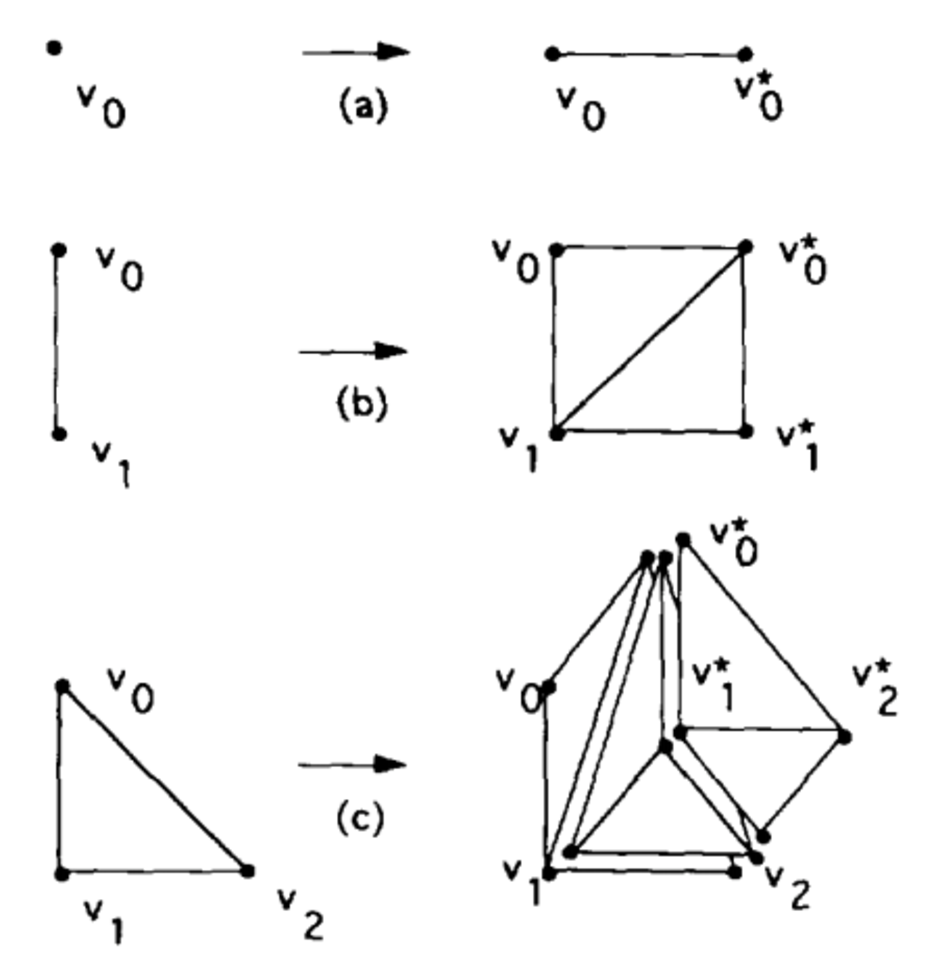
\includegraphics[width=0.8\linewidth]{images/extrusion}
	\end{minipage} 
   \label{fig:extrusion}
\end{figure}

In our implementation the combinatorial algorithm above is twofold generalised:
\begin{enumerate}
\item by applying it to all $d$-simplices of a LAR model of dimension $d$;
\item by using instead of the single interval $I=[0,1]$, the possibly unconnected set of 1D intervals generated by the list of integer numbers stored in the \texttt{pattern} variable
\end{enumerate}

\paragraph{Implementation}
In the macro below, \texttt{larExtrude} is the function to generate the output model vertices in a multiple extrusion of a LAR model.

First we notice that the \texttt{model} variable contains a pair (\texttt{V}, \texttt{FV}), where \texttt{V} is the array of input vertices, and \texttt{FV} is the array of $d$-cells (given as lists of vertex indices) providing the  input representation of a LAR cellular complex.

The \texttt{pattern} variable is a list of integers, whose absolute values provide the sizes of the ordered set of 1D (in local coords) subintervals specified by the \texttt{pattern} itself. Such subintervals are assembled in global coordinates, and each one of them is considered either solid or void depending on the sign of the corresponding integer, which may be either positive (solid subinterval) or negative (void subinterval).  

Therefore, a value \texttt{pattern = [1,1,-1,1]} must be interpreted as the 1D simplicial complex
\[
[0,1] \cup [1,2] \cup [3,4]
\]
with five vertices \texttt{W = [[0.0], [1.0], [2.0], [3.0], [4.0]]} and three $1$-cells \texttt{[[0,1], [1,2], [3,4]]}.

\texttt{V} is the list of input $d$-vertices (each given as a list of $d$ coordinates);
\texttt{coords} is a list of absolute translation parameters to be applied to \texttt{V} in order to generate the output vertices generated by the combinatorial extrusion algorithm.

The \texttt{cellGroups} variable is used to select the groups of $(d+1)$-simplices corresponding to solid intervals in the input \texttt{pattern}, and \texttt{CAT} provides to flatten their set, by removing a level of square brackets.

%-------------------------------------------------------------------------------
\begin{flushleft} \small
\begin{minipage}{\linewidth} \label{scrap1}
\protect\makebox[0ex][r]{\NWtarget{nuweb4a}{\rule{0ex}{0ex}}\hspace{1em}}$\langle\,$Simplicial model extrusion in accord with a 1D pattern\nobreak\ {\footnotesize 4a}$\,\rangle\equiv$
\vspace{-1ex}
\begin{list}{}{} \item
\mbox{}\verb@def larExtrude(model,pattern):@\\
\mbox{}\verb@    V, FV = model@\\
\mbox{}\verb@    d, m = len(FV[0]), len(pattern)@\\
\mbox{}\verb@    coords = list(cumsum([0]+(AA(ABS)(pattern))))@\\
\mbox{}\verb@    offset, outcells, rangelimit = len(V), [], d*m@\\
\mbox{}\verb@    for cell in FV:@\\
\mbox{}\verb@        @\hbox{$\langle\,$Append a chain of extruded cells to outcells\nobreak\ {\footnotesize \NWlink{nuweb4b}{4b}}$\,\rangle$}\verb@@\\
\mbox{}\verb@    outcells = AA(CAT)(TRANS(outcells))@\\
\mbox{}\verb@    cellGroups = [group for k,group in enumerate(outcells) if pattern[k]>0 ]@\\
\mbox{}\verb@    outVertices = [v+[z] for z in coords for v in V]@\\
\mbox{}\verb@    outModel = outVertices, CAT(cellGroups)@\\
\mbox{}\verb@    return outModel@\\
\mbox{}\verb@@{\NWsep}
\end{list}
\vspace{-1ex}
\footnotesize\addtolength{\baselineskip}{-1ex}
\begin{list}{}{\setlength{\itemsep}{-\parsep}\setlength{\itemindent}{-\leftmargin}}
\item \NWtxtMacroRefIn\ \NWlink{nuweb9b}{9b}.
\end{list}
\end{minipage}\\[4ex]
\end{flushleft}
%-------------------------------------------------------------------------------

\paragraph{Extrusion of single cells}
For each cell in \texttt{FV} a chain of vertices is created, then they are separated into groups of $d+1$ consecutive elements, by shifting one position at a time.

%-------------------------------------------------------------------------------
\begin{flushleft} \small
\begin{minipage}{\linewidth} \label{scrap2}
\protect\makebox[0ex][r]{\NWtarget{nuweb4b}{\rule{0ex}{0ex}}\hspace{1em}}$\langle\,$Append a chain of extruded cells to outcells\nobreak\ {\footnotesize 4b}$\,\rangle\equiv$
\vspace{-1ex}
\begin{list}{}{} \item
\mbox{}\verb@@\hbox{$\langle\,$Create the indices of vertices in the cell "tube"\nobreak\ {\footnotesize \NWlink{nuweb4c}{4c}}$\,\rangle$}\verb@@\\
\mbox{}\verb@@\hbox{$\langle\,$Take groups of d+1 elements, by shifting one position\nobreak\ {\footnotesize \NWlink{nuweb4d}{4d}}$\,\rangle$}\verb@   @\\
\mbox{}\verb@@{\NWsep}
\end{list}
\vspace{-1ex}
\footnotesize\addtolength{\baselineskip}{-1ex}
\begin{list}{}{\setlength{\itemsep}{-\parsep}\setlength{\itemindent}{-\leftmargin}}
\item \NWtxtMacroRefIn\ \NWlink{nuweb4a}{4a}.
\end{list}
\end{minipage}\\[4ex]
\end{flushleft}
%-------------------------------------------------------------------------------

\paragraph{Assembling vertex indices in a tube with their shifted images}
Here the ``long'' chain of vertices is created.
%-------------------------------------------------------------------------------
\begin{flushleft} \small
\begin{minipage}{\linewidth} \label{scrap3}
\protect\makebox[0ex][r]{\NWtarget{nuweb4c}{\rule{0ex}{0ex}}\hspace{1em}}$\langle\,$Create the indices of vertices in the cell "tube"\nobreak\ {\footnotesize 4c}$\,\rangle\equiv$
\vspace{-1ex}
\begin{list}{}{} \item
\mbox{}\verb@tube = [v + k*offset for k in range(m+1) for v in cell]  @{\NWsep}
\end{list}
\vspace{-1ex}
\footnotesize\addtolength{\baselineskip}{-1ex}
\begin{list}{}{\setlength{\itemsep}{-\parsep}\setlength{\itemindent}{-\leftmargin}}
\item \NWtxtMacroRefIn\ \NWlink{nuweb4b}{4b}.
\end{list}
\end{minipage}\\[4ex]
\end{flushleft}
%-------------------------------------------------------------------------------

\paragraph{Selecting and reshaping extruded cells in a tube}
Here the chain of vertices is spitted into subchains, and such subchains are reshaped into three-dimensional arrays of indices.
%-------------------------------------------------------------------------------
\begin{flushleft} \small
\begin{minipage}{\linewidth} \label{scrap4}
\protect\makebox[0ex][r]{\NWtarget{nuweb4d}{\rule{0ex}{0ex}}\hspace{1em}}$\langle\,$Take groups of d+1 elements, by shifting one position\nobreak\ {\footnotesize 4d}$\,\rangle\equiv$
\vspace{-1ex}
\begin{list}{}{} \item
\mbox{}\verb@cellTube = [tube[k:k+d+1] for k in range(rangelimit)]@\\
\mbox{}\verb@outcells += [reshape(cellTube, newshape=(m,d,d+1)).tolist()]   @{\NWsep}
\end{list}
\vspace{-1ex}
\footnotesize\addtolength{\baselineskip}{-1ex}
\begin{list}{}{\setlength{\itemsep}{-\parsep}\setlength{\itemindent}{-\leftmargin}}
\item \NWtxtMacroRefIn\ \NWlink{nuweb4b}{4b}.
\end{list}
\end{minipage}\\[4ex]
\end{flushleft}
%-------------------------------------------------------------------------------



\begin{definition}[Big-Omega order]
We say that a function $f(n)$ is \emph{Big-Omega} order of a function $f(n)$, and write 
$f(n) \in \Omega(g(n))$ when a constant $c$ exists, such that:
\[
\lim_{n\to\infty} \frac{f(n)}{g(n)}=c>0,\qquad \mbox{where\ } 0<c\leq\infty.
\]
\end{definition}



\begin{theorem}[Optimality]
The combinatorial algorithm for extrusion of simplicial complexes has time complexity $\Omega(n)$.
\end{theorem}
\proof{
Of course, if we denote as $g(n) = nd$ the time needed to write the input of the extrusion algorithm, proportional to the constant length $d$ of cells, and as $f(m) = m(d+1)$ the time needed to write the output, where $m=n(d+1)$, we have
\[
\lim_{n\to\infty} \frac{f(n)}{g(n)}= \lim_{n\to\infty} \frac{m(d+1)}{nd}
= \lim_{n\to\infty} \frac{[n(d+1)](d+1)}{nd} = \frac{(d+1)^2}{d} = c > 0
\]
\qed}

\subsubsection{Examples of simplicial complex extrusions}

\paragraph{Example 1}
It is interesting to notice that the 2D model extruded in example 1 below and shown in Figure~\ref{fig:assembly} is locally non-manifold, and that several instance of the pattern in the $z$ direction are obtained by just inserting a void subinterval (negative size) in the \texttt{pattern} value.

\begin{figure}[htbp] %  figure placement: here, top, bottom, or page
   \centering
   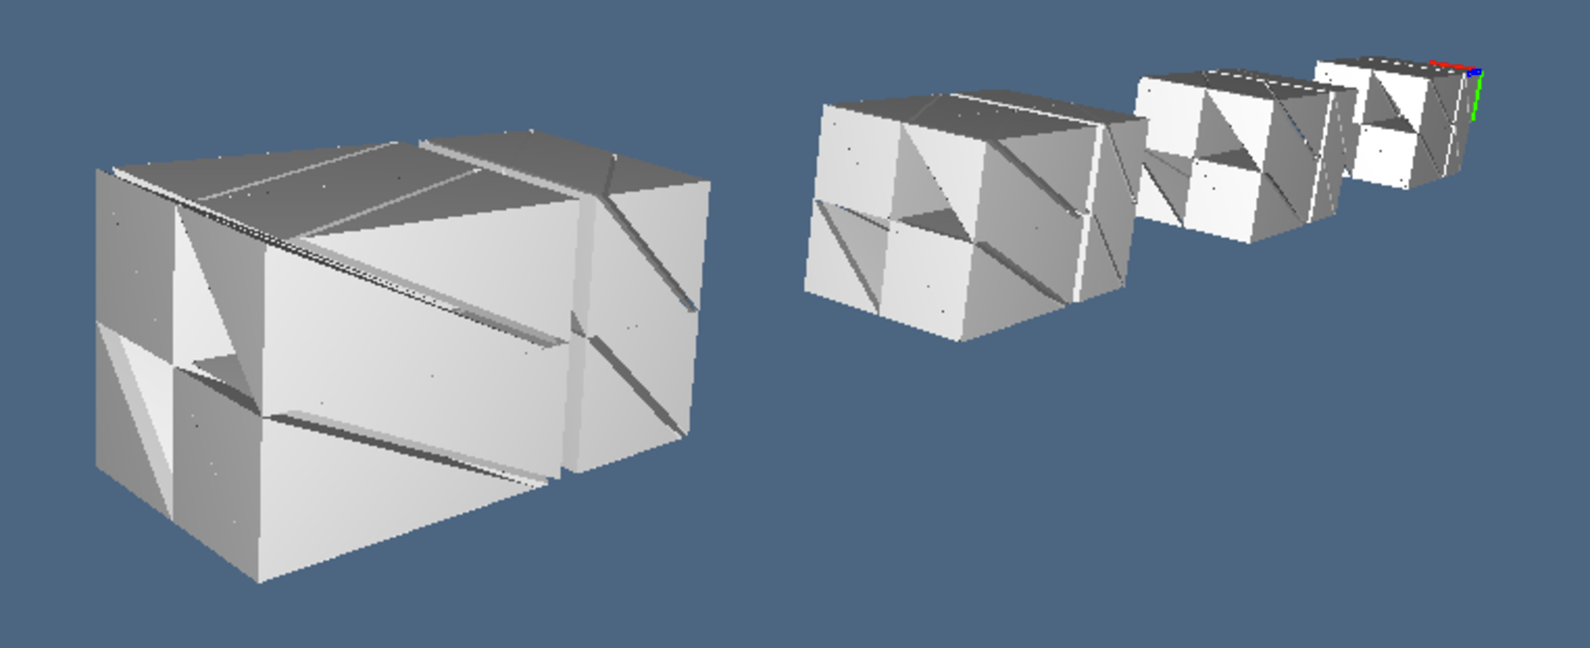
\includegraphics[width=0.7\linewidth]{images/assembly} 
   \caption{A simplicial complex providing a quite complex 3D assembly of tetrahedra.}
   \label{fig:assembly}
\end{figure}

\paragraph{Examples 2 and 3}
The examples show that the implemented \texttt{larExtrude} algorithm is fully multidimensional. 
It may be worth noting the initial definition of the empty \texttt{model}, as a pair having the empty list as vertex set and the list \texttt{[[0]]} as the cell list. Such initial value is used
to define a predefinite constant \texttt{VOID}.

\begin{figure}[htbp] %  figure placement: here, top, bottom, or page
   \centering
   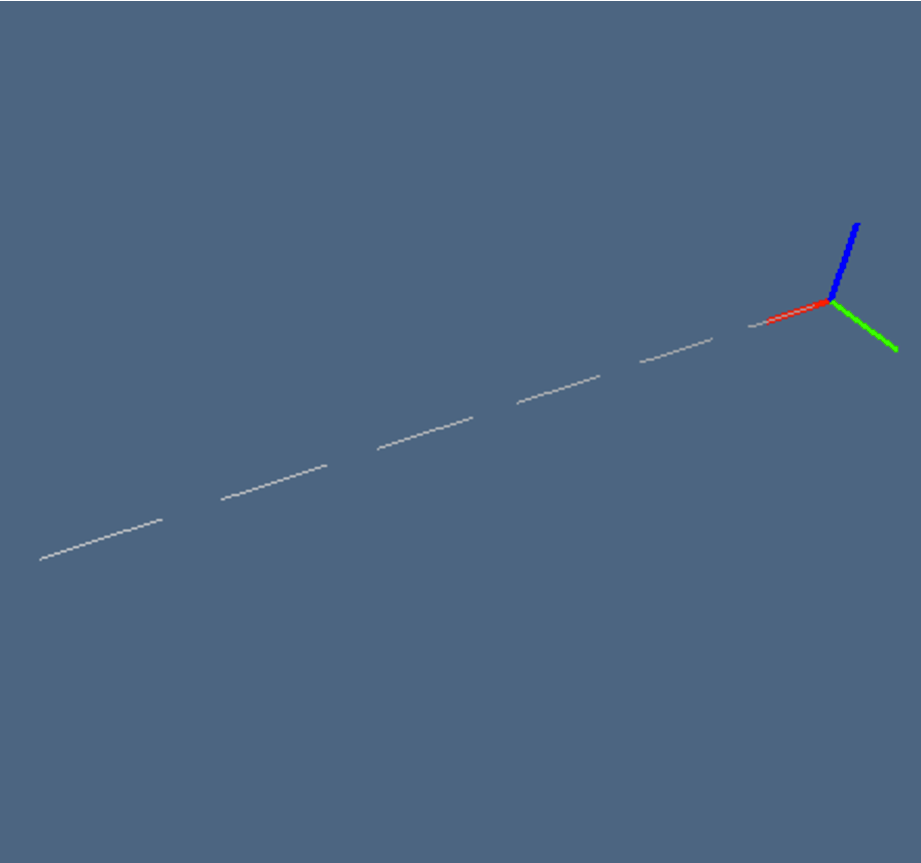
\includegraphics[height=0.25\linewidth,width=0.25\linewidth]{images/simplexn-1a} 
   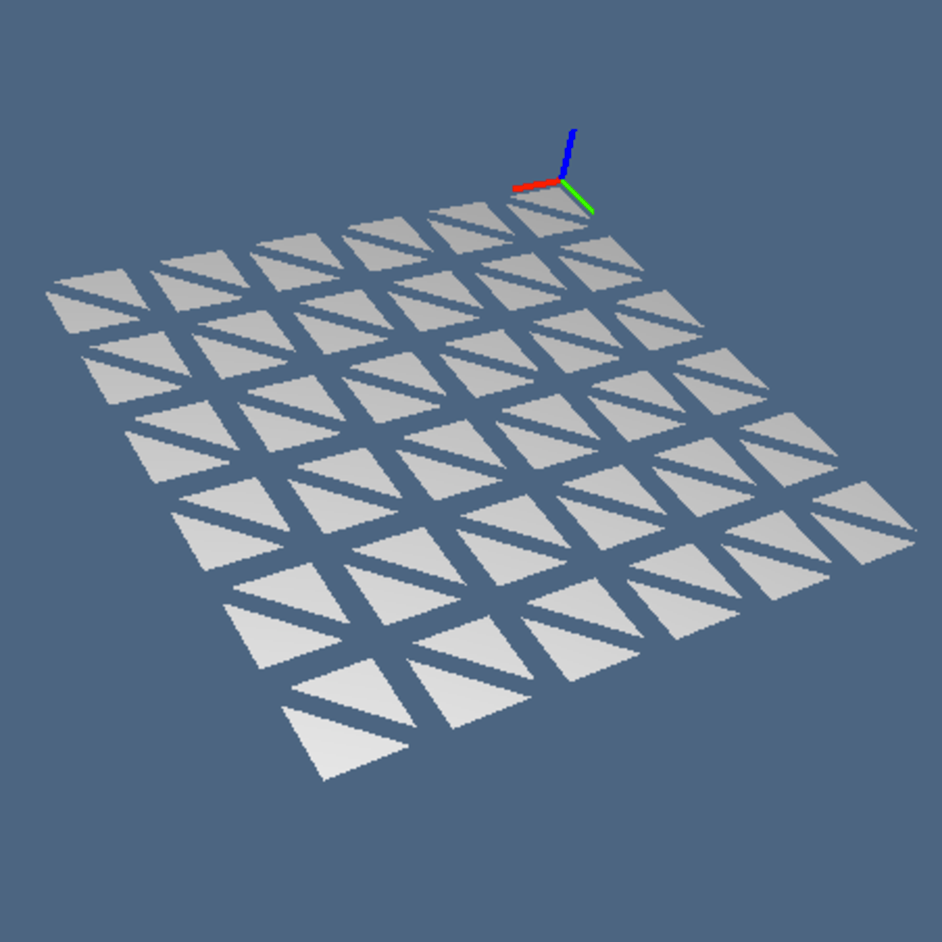
\includegraphics[height=0.25\linewidth,width=0.25\linewidth]{images/simplexn-1b} 
   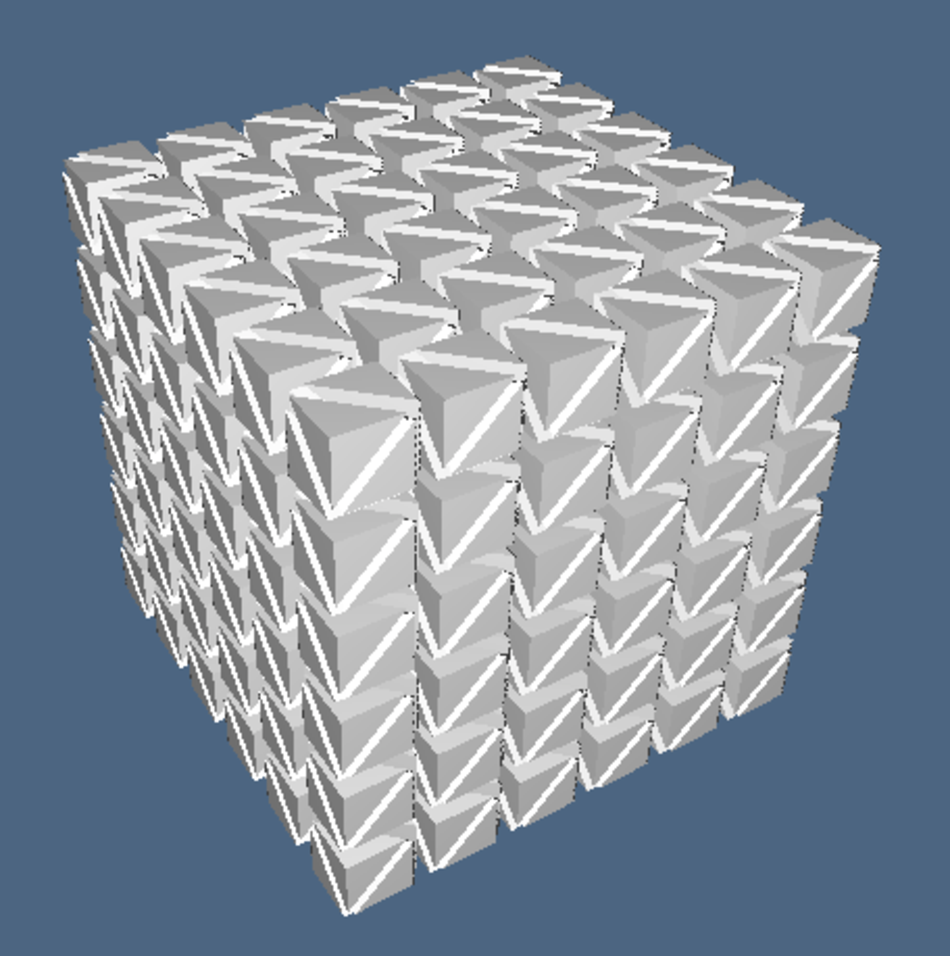
\includegraphics[height=0.25\linewidth,width=0.25\linewidth]{images/simplexn-1c} 
   \caption{1-, 2-, and 3-dimensional simplicial complex generated by repeated extrusion with the same pattern.}
   \label{fig:example}
\end{figure}

%-------------------------------------------------------------------------------
\begin{flushleft} \small \label{scrap5}
\protect\makebox[0ex][r]{\NWtarget{nuweb5}{\rule{0ex}{0ex}}\hspace{1em}}$\langle\,$Examples of simplicial complex extrusions\nobreak\ {\footnotesize 5}$\,\rangle\equiv$
\vspace{-1ex}
\begin{list}{}{} \item
\mbox{}\verb@# example 1@\\
\mbox{}\verb@V = [[0,0],[1,0],[2,0],[0,1],[1,1],[2,1],[0,2],[1,2],[2,2]]@\\
\mbox{}\verb@FV = [[0,1,3],[1,2,4],[2,4,5],[3,4,6],[4,6,7],[5,7,8]]@\\
\mbox{}\verb@model = larExtrude((V,FV),4*[1,2,-3])@\\
\mbox{}\verb@VIEW(EXPLODE(1,1,1.2)(MKPOLS(model)))@\\
\mbox{}\verb@@\\
\mbox{}\verb@# example 2@\\
\mbox{}\verb@model = larExtrude( VOID, 6*[1] )@\\
\mbox{}\verb@VIEW(EXPLODE(1.5,1.5,1.5)(MKPOLS(model)))@\\
\mbox{}\verb@model = larExtrude( model, 6*[1] )@\\
\mbox{}\verb@VIEW(EXPLODE(1.5,1.5,1.5)(MKPOLS(model)))@\\
\mbox{}\verb@model = larExtrude( model, 6*[1] )@\\
\mbox{}\verb@VIEW(EXPLODE(1.5,1.5,1.5)(MKPOLS(model)))@\\
\mbox{}\verb@@\\
\mbox{}\verb@# example 3@\\
\mbox{}\verb@model = larExtrude( VOID, 10*[1,-1] )@\\
\mbox{}\verb@VIEW(EXPLODE(1.5,1.5,1.5)(MKPOLS(model)))@\\
\mbox{}\verb@model = larExtrude( model, 10*[1] )@\\
\mbox{}\verb@VIEW(EXPLODE(1.5,1.5,1.5)(MKPOLS(model)))@\\
\mbox{}\verb@@{\NWsep}
\end{list}
\vspace{-1ex}
\footnotesize\addtolength{\baselineskip}{-1ex}
\begin{list}{}{\setlength{\itemsep}{-\parsep}\setlength{\itemindent}{-\leftmargin}}
\item \NWtxtMacroRefIn\ \NWlink{nuweb9b}{9b}.
\end{list}
\end{flushleft}
%-------------------------------------------------------------------------------


\begin{figure}[htbp] %  figure placement: here, top, bottom, or page
   \centering
   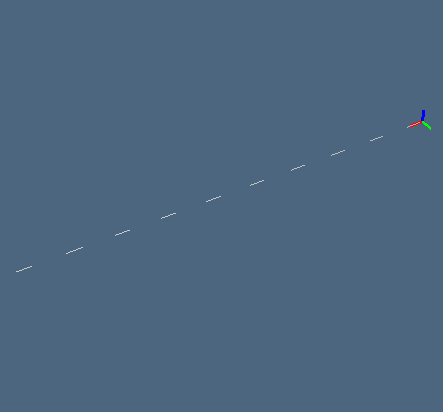
\includegraphics[height=0.25\linewidth,width=0.25\linewidth]{images/simplexn-2a} 
   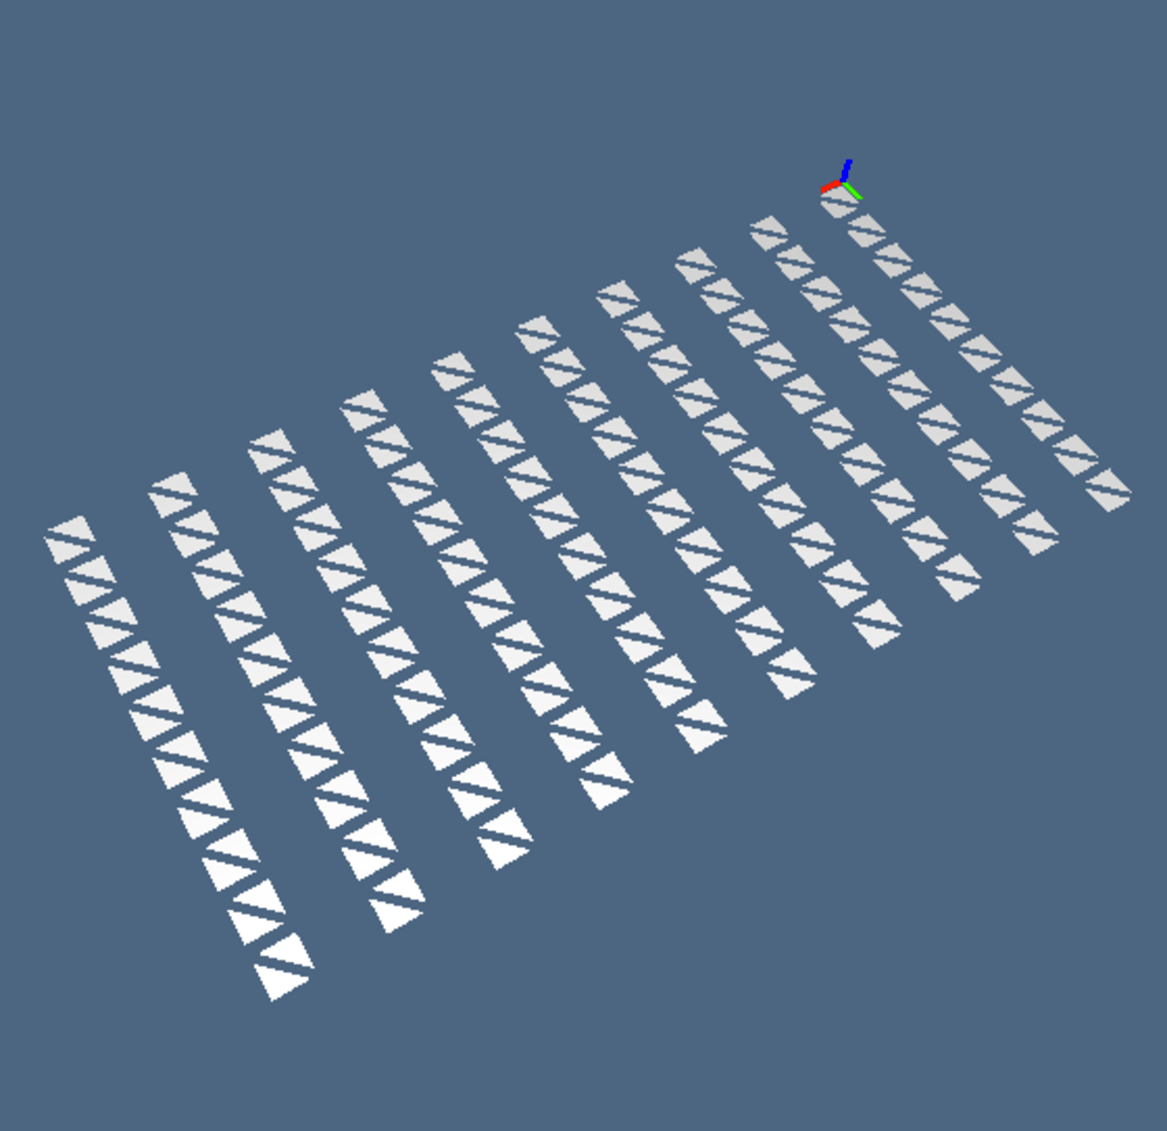
\includegraphics[height=0.25\linewidth,width=0.25\linewidth]{images/simplexn-2b} 
   \caption{1- and 2-dimensional simplicial complexes generated by different patterns.}
   \label{fig:example}
\end{figure}


\subsection{Generation of multidimensional simplicial grids}

The generation of simplicial grids of any dimension and shape using the \texttt{larSimplexGrid}
is amazingly simple. The input parameter \texttt{shape} is either a tuple or a list of integers used to specify the \emph{shape} of the created array, i.e.~both the number of its dimensions (given by \texttt{len(shape)}) and the \texttt{size} of each dimension $k$ (given by the \texttt{shape[k]} element).
The implementation starts from the LAR model of the VOID simplicial complex (denoted as \texttt{VOID}, a predefined constant) and updates the \texttt{model} variable extruding it iteratively according to the specs given by \texttt{shape}.
Just notice that the returned grid \texttt{model} has vertices with integer coordinates, that can be subsequently scaled and/or translated and/or mapped in any other way, according to the user needs.

%-------------------------------------------------------------------------------
\begin{flushleft} \small
\begin{minipage}{\linewidth} \label{scrap6}
\protect\makebox[0ex][r]{\NWtarget{nuweb7}{\rule{0ex}{0ex}}\hspace{1em}}$\langle\,$Generation of simplicial grids\nobreak\ {\footnotesize 7}$\,\rangle\equiv$
\vspace{-1ex}
\begin{list}{}{} \item
\mbox{}\verb@def larSimplexGrid(shape):@\\
\mbox{}\verb@    model = VOID@\\
\mbox{}\verb@    for item in shape:@\\
\mbox{}\verb@        model = larExtrude(model,item*[1])@\\
\mbox{}\verb@    return model@\\
\mbox{}\verb@@{\NWsep}
\end{list}
\vspace{-1ex}
\footnotesize\addtolength{\baselineskip}{-1ex}
\begin{list}{}{\setlength{\itemsep}{-\parsep}\setlength{\itemindent}{-\leftmargin}}
\item \NWtxtMacroRefIn\ \NWlink{nuweb9b}{9b}.
\end{list}
\end{minipage}\\[4ex]
\end{flushleft}
%-------------------------------------------------------------------------------


\paragraph{Examples of simplicial grids} The two examples of simplicial grids generated by the macro below with \texttt{shape} equal to \texttt{[3,3]} and \texttt{[2,3,4]}, respectively, are displayed in Figure~\ref{fig:simplexn-3}.

\begin{figure}[htbp] %  figure placement: here, top, bottom, or page
   \centering
   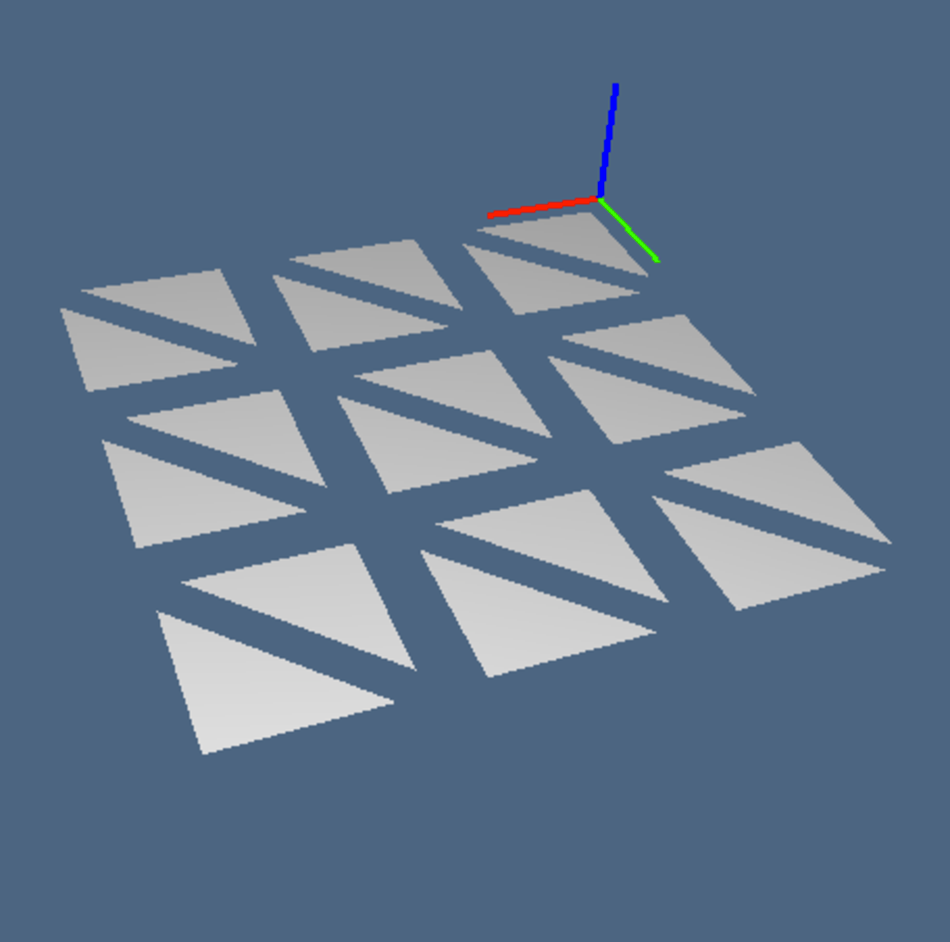
\includegraphics[height=0.25\linewidth,width=0.25\linewidth]{images/simplexn-3a} 
   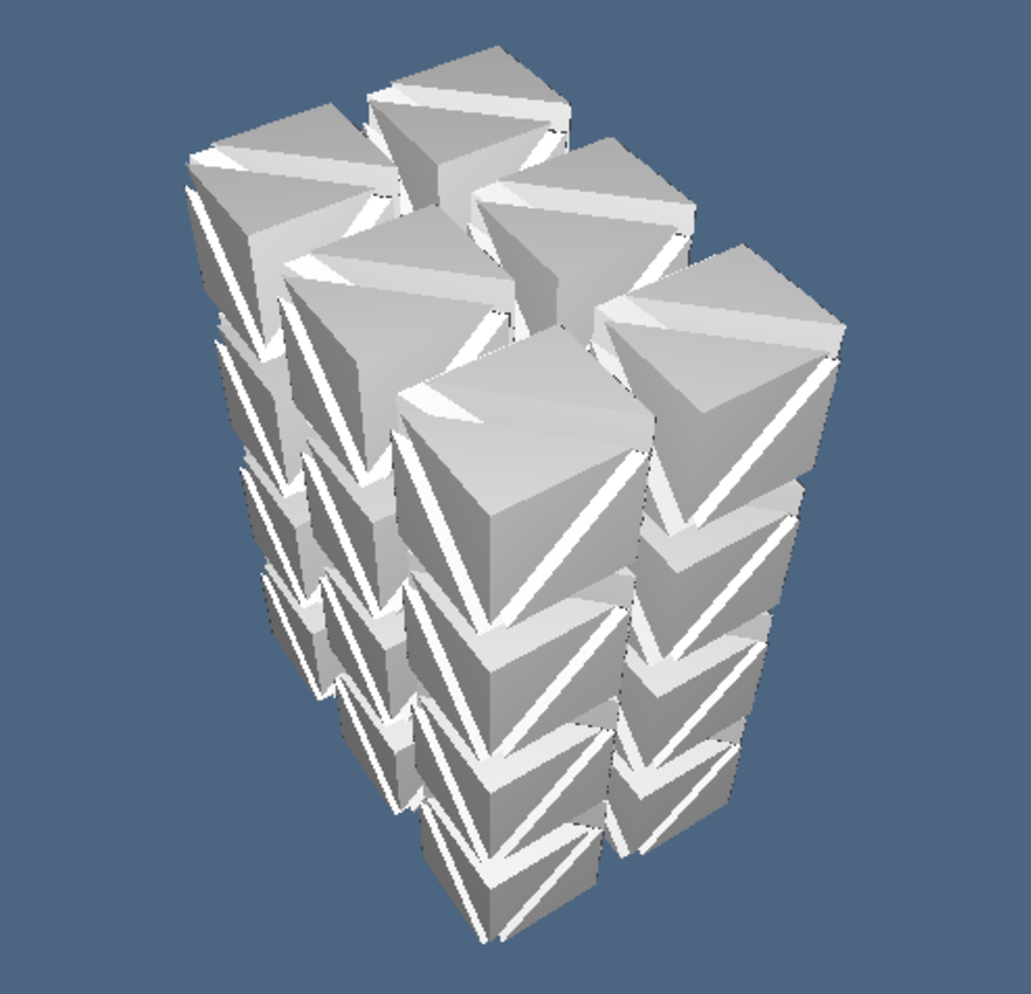
\includegraphics[height=0.25\linewidth,width=0.25\linewidth]{images/simplexn-3b} 
   \caption{2- and 3-dimensional simplicial grids.}
   \label{fig:simplexn-3}
\end{figure}

%-------------------------------------------------------------------------------
\begin{flushleft} \small
\begin{minipage}{\linewidth} \label{scrap7}
\protect\makebox[0ex][r]{\NWtarget{nuweb8a}{\rule{0ex}{0ex}}\hspace{1em}}$\langle\,$Examples of simplicial grids\nobreak\ {\footnotesize 8a}$\,\rangle\equiv$
\vspace{-1ex}
\begin{list}{}{} \item
\mbox{}\verb@grid_2d = larSimplexGrid([3,3])@\\
\mbox{}\verb@VIEW(EXPLODE(1.5,1.5,1.5)(MKPOLS(grid_2d)))@\\
\mbox{}\verb@@\\
\mbox{}\verb@grid_3d = larSimplexGrid([2,3,4])@\\
\mbox{}\verb@VIEW(EXPLODE(1.5,1.5,1.5)(MKPOLS(grid_3d)))@\\
\mbox{}\verb@@{\NWsep}
\end{list}
\vspace{-1ex}
\footnotesize\addtolength{\baselineskip}{-1ex}
\begin{list}{}{\setlength{\itemsep}{-\parsep}\setlength{\itemindent}{-\leftmargin}}
\item \NWtxtMacroRefIn\ \NWlink{nuweb9b}{9b}.
\end{list}
\end{minipage}\\[4ex]
\end{flushleft}
%-------------------------------------------------------------------------------


\subsection{Facet extraction from simplices}

A $k$-face of a $d$-simplex is defined as the convex hull of any subset of $k$ vertices.
A $(d-1)$-face of a $d$-simplex 
\[
\sigma^d = \langle v_0, v_1, \ldots, v_d \rangle
\]
 is also called a \emph{facet}. Each of the $d+1$ facets of $\sigma^d$, obtained by removing a vertex from $\sigma^d$, is a $(d-1)$-simplex. A simplex may be oriented in two different ways according to the permutation
class of its vertices. The simplex \emph{orientation} is so changed by either multiplying the simplex by -1, or by executing an odd number of exchanges of its vertices. 

The chain of oriented boundary facets of $\sigma^d$, usually denoted as $\partial \sigma^d$, is generated combinatorially as follows:
\[
\partial\, \sigma^d = \sum_{k=0}^d (-1)^d \langle v_0, \ldots, v_{k-1}, v_{k+1}, \ldots, v_d \rangle
\]

\paragraph{Implementation}

The \texttt{larSimplexFacets} function, for estraction of non-oriented $(d-1)$-facets of $d$-dimensional simplices, returns a list of $d$-tuples of integers, i.e.~the input LAR representation of the topology of a cellular complex. The final \emph{list comprehension} is used to remove the duplicated facets, by taking only the last element of any subsequence with possibly duplicated elements.
        
%-------------------------------------------------------------------------------
\begin{flushleft} \small
\begin{minipage}{\linewidth} \label{scrap8}
\protect\makebox[0ex][r]{\NWtarget{nuweb8b}{\rule{0ex}{0ex}}\hspace{1em}}$\langle\,$Facets extraction from a set of simplices\nobreak\ {\footnotesize 8b}$\,\rangle\equiv$
\vspace{-1ex}
\begin{list}{}{} \item
\mbox{}\verb@def larSimplexFacets(simplices):@\\
\mbox{}\verb@    out = []@\\
\mbox{}\verb@    d = len(simplices[0])@\\
\mbox{}\verb@    for simplex in simplices:@\\
\mbox{}\verb@        out += [simplex[0:k]+simplex[k+1:d] for k in range(d)]@\\
\mbox{}\verb@    out = sorted(out)@\\
\mbox{}\verb@    return [facet for k,facet in enumerate(out[:-1]) if out[k] != out[k+1]] \@\\
\mbox{}\verb@      + [out[-1]] @\\
\mbox{}\verb@@{\NWsep}
\end{list}
\vspace{-1ex}
\footnotesize\addtolength{\baselineskip}{-1ex}
\begin{list}{}{\setlength{\itemsep}{-\parsep}\setlength{\itemindent}{-\leftmargin}}
\item \NWtxtMacroRefIn\ \NWlink{nuweb9b}{9b}.
\end{list}
\end{minipage}\\[4ex]
\end{flushleft}
%-------------------------------------------------------------------------------

\paragraph{Examples of facet extraction}
The simple generation of the LAR model of a simplicial decomposition of a 3D cube as a \texttt{larSimplexGrid} with \texttt{shape = [1,1,1]} and of its 2D and 1D skeletons is shown here.

%-------------------------------------------------------------------------------
\begin{flushleft} \small
\begin{minipage}{\linewidth} \label{scrap9}
\protect\makebox[0ex][r]{\NWtarget{nuweb9a}{\rule{0ex}{0ex}}\hspace{1em}}$\langle\,$Examples of facet extraction from 3D simplicial cube\nobreak\ {\footnotesize 9a}$\,\rangle\equiv$
\vspace{-1ex}
\begin{list}{}{} \item
\mbox{}\verb@V,CV = larSimplexGrid([1,1,1])@\\
\mbox{}\verb@VIEW(EXPLODE(1.5,1.5,1.5)(MKPOLS((V,CV))))@\\
\mbox{}\verb@SK2 = (V,larSimplexFacets(CV))@\\
\mbox{}\verb@VIEW(EXPLODE(1.5,1.5,1.5)(MKPOLS(SK2)))@\\
\mbox{}\verb@SK1 = (V,larSimplexFacets(SK2[1]))@\\
\mbox{}\verb@VIEW(EXPLODE(1.5,1.5,1.5)(MKPOLS(SK1)))@\\
\mbox{}\verb@@{\NWsep}
\end{list}
\vspace{-1ex}
\footnotesize\addtolength{\baselineskip}{-1ex}
\begin{list}{}{\setlength{\itemsep}{-\parsep}\setlength{\itemindent}{-\leftmargin}}
\item \NWtxtMacroRefIn\ \NWlink{nuweb9b}{9b}.
\end{list}
\end{minipage}\\[4ex]
\end{flushleft}
%-------------------------------------------------------------------------------



\subsection{Exporting the $Simple_x^n$ library}
The current version of the \texttt{simplexn} library is exported here. Next versions will take care of the OpenCL acceleration and data partitioning with very-large size simplicial grids and their sets of faces.

%-------------------------------------------------------------------------------
\begin{flushleft} \small
\begin{minipage}{\linewidth} \label{scrap10}
\protect\makebox[0ex][r]{\NWtarget{nuweb9b}{\rule{0ex}{0ex}}\hspace{1em}}\verb@"lib/py/simplexn.py"@\nobreak\ {\footnotesize 9b }$\equiv$
\vspace{-1ex}
\begin{list}{}{} \item
\mbox{}\verb@# -*- coding: utf-8 -*-@\\
\mbox{}\verb@"""Module for facet extraction, extrusion and simplicial grids"""@\\
\mbox{}\verb@from pyplasm import *@\\
\mbox{}\verb@from lar2psm import *@\\
\mbox{}\verb@from scipy import *@\\
\mbox{}\verb@@\\
\mbox{}\verb@VOID = V0,CV0 = [[]],[[0]]    # the empty simplicial model@\\
\mbox{}\verb@@\hbox{$\langle\,$Cumulative sum\nobreak\ {\footnotesize \NWlink{nuweb12a}{12a}}$\,\rangle$}\verb@@\\
\mbox{}\verb@@\hbox{$\langle\,$Simplicial model extrusion in accord with a 1D pattern\nobreak\ {\footnotesize \NWlink{nuweb4a}{4a}}$\,\rangle$}\verb@@\\
\mbox{}\verb@@\hbox{$\langle\,$Generation of simplicial grids\nobreak\ {\footnotesize \NWlink{nuweb7}{7}}$\,\rangle$}\verb@@\\
\mbox{}\verb@@\hbox{$\langle\,$Facets extraction from a set of simplices\nobreak\ {\footnotesize \NWlink{nuweb8b}{8b}}$\,\rangle$}\verb@@\\
\mbox{}\verb@if __name__ == "__main__":@\\
\mbox{}\verb@   @\hbox{$\langle\,$Examples of simplicial complex extrusions\nobreak\ {\footnotesize \NWlink{nuweb5}{5}}$\,\rangle$}\verb@@\\
\mbox{}\verb@   @\hbox{$\langle\,$Examples of simplicial grids\nobreak\ {\footnotesize \NWlink{nuweb8a}{8a}}$\,\rangle$}\verb@@\\
\mbox{}\verb@   @\hbox{$\langle\,$Examples of facet extraction from 3D simplicial cube\nobreak\ {\footnotesize \NWlink{nuweb9a}{9a}}$\,\rangle$}\verb@@\\
\mbox{}\verb@@{\NWsep}
\end{list}
\vspace{-2ex}
\end{minipage}\\[4ex]
\end{flushleft}
%-------------------------------------------------------------------------------


\section{Signed (co)boundary matrices of a simplicial complex}
\label{simplicial}

\section{Test examples}

\subsection{Structured grid}

\subsubsection{2D example}

\paragraph{Generate a simplicial decomposition}
Then we generate and show a 2D decomposition of the unit square $[0,1]^2\subset\E^2$ into a $3\times 3$ grid of simplices (triangles, in this case), using the \texttt{larSimplexGrid} function, that returns a pair \texttt{(V,FV)}, made by the array \texttt{V} of vertices, and by the array \texttt{FV} of ``faces by vertex'' indices, that constitute a \emph{reduced} simplicial LAR of the $[0,1]^2$ domain. The computed \texttt{FV} array is then dispayed ``exploded'', being $ex,ey,ez$ the explosion parameters in the $x,y,z$ coordinate directions, respectively. Notice that the \texttt{MKPOLS} pyplasm primitive requires a pair \texttt{(V,FV)}, that we call a ``model'', as input --- i.e. a pair made by the array \texttt{V} of vertices, and by a zero-based array of array of indices of vertices. Elsewhere in this document we identified such a data structure as CSR$(M_d)$, for some dimension $d$. Suc notation stands for the Compressed Sparse Row representation of a binary characteristic matrix.

\begin{flushleft} \small
\begin{minipage}{\linewidth} \label{scrap11}
\protect\makebox[0ex][r]{\NWtarget{nuweb10a}{\rule{0ex}{0ex}}\hspace{1em}}$\langle\,$Generate a simplicial decomposition ot the $[0,1]^2$ domain\nobreak\ {\footnotesize 10a}$\,\rangle\equiv$
\vspace{-1ex}
\begin{list}{}{} \item
\mbox{}\verb@V,FV = larSimplexGrid([3,3])@\\
\mbox{}\verb@VIEW(EXPLODE(1.5,1.5,1.5)(MKPOLS((V,FV))))@\\
\mbox{}\verb@@{\NWsep}
\end{list}
\vspace{-1ex}
\footnotesize\addtolength{\baselineskip}{-1ex}
\begin{list}{}{\setlength{\itemsep}{-\parsep}\setlength{\itemindent}{-\leftmargin}}
\item \NWtxtMacroRefIn\ \NWlink{nuweb10c}{10c}.
\end{list}
\end{minipage}\\[4ex]
\end{flushleft}
\paragraph{Extract the $(d-1)$-faces}
Since the complex is simplicial, we can directly extract its facets (in this case the 1-faces, i.e. its edges) by invoking the \texttt{larSimplexFacets} function on the argument \texttt{FV}, so returning the array \texttt{EV} of ``edges by vertex'' indices. 

%-------------------------------------------------------------------------------
\begin{flushleft} \small
\begin{minipage}{\linewidth} \label{scrap12}
\protect\makebox[0ex][r]{\NWtarget{nuweb10b}{\rule{0ex}{0ex}}\hspace{1em}}$\langle\,$Extract the edges of the 2D decomposition\nobreak\ {\footnotesize 10b}$\,\rangle\equiv$
\vspace{-1ex}
\begin{list}{}{} \item
\mbox{}\verb@EV = larSimplexFacets(FV)@\\
\mbox{}\verb@ex,ey,ez = 1.5,1.5,1.5@\\
\mbox{}\verb@VIEW(EXPLODE(ex,ey,ez)(MKPOLS((V,EV))))@\\
\mbox{}\verb@@{\NWsep}
\end{list}
\vspace{-1ex}
\footnotesize\addtolength{\baselineskip}{-1ex}
\begin{list}{}{\setlength{\itemsep}{-\parsep}\setlength{\itemindent}{-\leftmargin}}
\item \NWtxtMacroRefIn\ \NWlink{nuweb10c}{10c}.
\end{list}
\end{minipage}\\[4ex]
\end{flushleft}
%-------------------------------------------------------------------------------

\paragraph{Export the executable file}
We are finally able to generate and output a complete test file, including the visualization expressions. This file can be executed by the \texttt{test} target of the \texttt{make} command.

%-------------------------------------------------------------------------------
\begin{flushleft} \small \label{scrap13}
\protect\makebox[0ex][r]{\NWtarget{nuweb10c}{\rule{0ex}{0ex}}\hspace{1em}}\verb@"test/py/simplexn/test01.py"@\nobreak\ {\footnotesize 10c }$\equiv$
\vspace{-1ex}
\begin{list}{}{} \item
\mbox{}\verb@@\\
\mbox{}\verb@@\hbox{$\langle\,$Inport the $Simple_X^n$ library\nobreak\ {\footnotesize \NWlink{nuweb12b}{12b}}$\,\rangle$}\verb@@\\
\mbox{}\verb@@\hbox{$\langle\,$Generate a simplicial decomposition ot the $[0,1]^2$ domain\nobreak\ {\footnotesize \NWlink{nuweb10a}{10a}}$\,\rangle$}\verb@@\\
\mbox{}\verb@@\hbox{$\langle\,$Extract the edges of the 2D decomposition\nobreak\ {\footnotesize \NWlink{nuweb10b}{10b}}$\,\rangle$}\verb@@\\
\mbox{}\verb@@{\NWsep}
\end{list}
\vspace{-2ex}
\end{flushleft}
%-------------------------------------------------------------------------------

\subsubsection{3D example}

In this case we produce a $2\times 2\times 2$ grid of tetrahedra. The dimension (3D) of the model to be generated is inferred by the presence of 3 parameters in the parameter list of the \texttt{larSimplexGrid} function. 

%-------------------------------------------------------------------------------
\begin{flushleft} \small
\begin{minipage}{\linewidth} \label{scrap14}
\protect\makebox[0ex][r]{\NWtarget{nuweb11a}{\rule{0ex}{0ex}}\hspace{1em}}$\langle\,$Generate a simplicial decomposition ot the $[0,1]^3$ domain\nobreak\ {\footnotesize 11a}$\,\rangle\equiv$
\vspace{-1ex}
\begin{list}{}{} \item
\mbox{}\verb@V,CV = larSimplexGrid([2,2,2])@\\
\mbox{}\verb@VIEW(EXPLODE(1.5,1.5,1.5)(MKPOLS((V,CV))))@\\
\mbox{}\verb@@{\NWsep}
\end{list}
\vspace{-1ex}
\footnotesize\addtolength{\baselineskip}{-1ex}
\begin{list}{}{\setlength{\itemsep}{-\parsep}\setlength{\itemindent}{-\leftmargin}}
\item \NWtxtMacroRefIn\ \NWlink{nuweb11c}{11c}.
\end{list}
\end{minipage}\\[4ex]
\end{flushleft}
%-------------------------------------------------------------------------------

and repeat two times the facet extraction:

%-------------------------------------------------------------------------------
\begin{flushleft} \small
\begin{minipage}{\linewidth} \label{scrap15}
\protect\makebox[0ex][r]{\NWtarget{nuweb11b}{\rule{0ex}{0ex}}\hspace{1em}}$\langle\,$Extract the faces and edges of the 3D decomposition\nobreak\ {\footnotesize 11b}$\,\rangle\equiv$
\vspace{-1ex}
\begin{list}{}{} \item
\mbox{}\verb@@\\
\mbox{}\verb@FV = larSimplexFacets(CV)@\\
\mbox{}\verb@VIEW(EXPLODE(1.5,1.5,1.5)(MKPOLS((V,FV))))@\\
\mbox{}\verb@EV = larSimplexFacets(FV)@\\
\mbox{}\verb@VIEW(EXPLODE(1.5,1.5,1.5)(MKPOLS((V,EV))))@\\
\mbox{}\verb@@{\NWsep}
\end{list}
\vspace{-1ex}
\footnotesize\addtolength{\baselineskip}{-1ex}
\begin{list}{}{\setlength{\itemsep}{-\parsep}\setlength{\itemindent}{-\leftmargin}}
\item \NWtxtMacroRefIn\ \NWlink{nuweb11c}{11c}.
\end{list}
\end{minipage}\\[4ex]
\end{flushleft}
%-------------------------------------------------------------------------------

and finally export a new test file:

%-------------------------------------------------------------------------------
\begin{flushleft} \small \label{scrap16}
\protect\makebox[0ex][r]{\NWtarget{nuweb11c}{\rule{0ex}{0ex}}\hspace{1em}}\verb@"test/py/simplexn/test02.py"@\nobreak\ {\footnotesize 11c }$\equiv$
\vspace{-1ex}
\begin{list}{}{} \item
\mbox{}\verb@@\\
\mbox{}\verb@@\hbox{$\langle\,$Inport the $Simple_X^n$ library\nobreak\ {\footnotesize \NWlink{nuweb12b}{12b}}$\,\rangle$}\verb@@\\
\mbox{}\verb@@\hbox{$\langle\,$Generate a simplicial decomposition ot the $[0,1]^3$ domain\nobreak\ {\footnotesize \NWlink{nuweb11a}{11a}}$\,\rangle$}\verb@@\\
\mbox{}\verb@@\hbox{$\langle\,$Extract the faces and edges of the 3D decomposition\nobreak\ {\footnotesize \NWlink{nuweb11b}{11b}}$\,\rangle$}\verb@@\\
\mbox{}\verb@@{\NWsep}
\end{list}
\vspace{-2ex}
\end{flushleft}
%-------------------------------------------------------------------------------


\subsection{Unstructured grid}


\subsubsection{2D example}


\subsubsection{3D example}


\appendix
\section{Utilities}


%-------------------------------------------------------------------------------
\begin{flushleft} \small
\begin{minipage}{\linewidth} \label{scrap17}
\protect\makebox[0ex][r]{\NWtarget{nuweb12a}{\rule{0ex}{0ex}}\hspace{1em}}$\langle\,$Cumulative sum\nobreak\ {\footnotesize 12a}$\,\rangle\equiv$
\vspace{-1ex}
\begin{list}{}{} \item
\mbox{}\verb@@\\
\mbox{}\verb@def cumsum(iterable):@\\
\mbox{}\verb@    # cumulative addition: list(cumsum(range(4))) => [0, 1, 3, 6]@\\
\mbox{}\verb@    iterable = iter(iterable)@\\
\mbox{}\verb@    s = iterable.next()@\\
\mbox{}\verb@    yield s@\\
\mbox{}\verb@    for c in iterable:@\\
\mbox{}\verb@        s = s + c@\\
\mbox{}\verb@        yield s@\\
\mbox{}\verb@@{\NWsep}
\end{list}
\vspace{-1ex}
\footnotesize\addtolength{\baselineskip}{-1ex}
\begin{list}{}{\setlength{\itemsep}{-\parsep}\setlength{\itemindent}{-\leftmargin}}
\item \NWtxtMacroRefIn\ \NWlink{nuweb9b}{9b}.
\end{list}
\end{minipage}\\[4ex]
\end{flushleft}
%-------------------------------------------------------------------------------


\begin{flushleft} \small
\begin{minipage}{\linewidth} \label{scrap18}
\protect\makebox[0ex][r]{\NWtarget{nuweb12b}{\rule{0ex}{0ex}}\hspace{1em}}$\langle\,$Inport the $Simple_X^n$ library\nobreak\ {\footnotesize 12b}$\,\rangle\equiv$
\vspace{-1ex}
\begin{list}{}{} \item
\mbox{}\verb@""" import modules from larcc/lib """@\\
\mbox{}\verb@import sys@\\
\mbox{}\verb@sys.path.insert(0, 'lib/py/')@\\
\mbox{}\verb@from pyplasm import *@\\
\mbox{}\verb@from lar2psm import *@\\
\mbox{}\verb@from simplexn import *@\\
\mbox{}\verb@@{\NWsep}
\end{list}
\vspace{-1ex}
\footnotesize\addtolength{\baselineskip}{-1ex}
\begin{list}{}{\setlength{\itemsep}{-\parsep}\setlength{\itemindent}{-\leftmargin}}
\item \NWtxtMacroRefIn\ \NWlink{nuweb10c}{10c}\NWlink{nuweb11c}{, 11c}.
\end{list}
\end{minipage}\\[4ex]
\end{flushleft}
\bibliographystyle{amsalpha}
\bibliography{simplexn}

\end{document}

% -------------------------------------------------------------------------
% ------ nuweb macros (redefine as desired, or omit with "nuweb -p") ------
% -------------------------------------------------------------------------
\providecommand{\NWtxtMacroDefBy}{Macro defined by}
\providecommand{\NWtxtMacroRefIn}{Macro referenced in}
\providecommand{\NWtxtMacroNoRef}{Macro never referenced}
\providecommand{\NWtxtDefBy}{Defined by}
\providecommand{\NWtxtRefIn}{Referenced in}
\providecommand{\NWtxtNoRef}{Not referenced}
\providecommand{\NWtxtFileDefBy}{File defined by}
\providecommand{\NWsep}{${\diamond}$}
\providecommand{\NWlink}[2]{\hyperlink{#1}{#2}}
\providecommand{\NWtarget}[2]{% move baseline up by \baselineskip 
  \raisebox{\baselineskip}[1.5ex][0ex]{%
    \mbox{%
      \hypertarget{#1}{%
        \raisebox{-1\baselineskip}[0ex][0ex]{%
          \mbox{#2}%
}}}}}
% -------------------------------------------------------------------------

\documentclass[11pt,oneside]{article}	%use"amsart"insteadof"article"forAMSLaTeXformat
\usepackage{geometry}		%Seegeometry.pdftolearnthelayoutoptions.Therearelots.
\geometry{letterpaper}		%...ora4paperora5paperor...
%\geometry{landscape}		%Activateforforrotatedpagegeometry
%\usepackage[parfill]{parskip}		%Activatetobeginparagraphswithanemptylineratherthananindent
\usepackage{graphicx}				%Usepdf,png,jpg,orepsßwithpdflatex;useepsinDVImode
								%TeXwillautomaticallyconverteps-->pdfinpdflatex		
\usepackage{amssymb}
\usepackage[colorlinks]{hyperref}

%----macros begin---------------------------------------------------------------
\usepackage{color}
\usepackage{amsthm}
\usepackage{amsmath}

\def\conv{\mbox{\textrm{conv}\,}}
\def\aff{\mbox{\textrm{aff}\,}}
\def\E{\mathbb{E}}
\def\R{\mathbb{R}}
\def\Z{\mathbb{Z}}
\def\tex{\TeX}
\def\latex{\LaTeX}
\def\v#1{{\bf #1}}
\def\p#1{{\bf #1}}
\def\T#1{{\bf #1}}

\def\vet#1{{\left(\begin{array}{cccccccccccccccccccc}#1\end{array}\right)}}
\def\mat#1{{\left(\begin{array}{cccccccccccccccccccc}#1\end{array}\right)}}

\def\lin{\mbox{\rm lin}\,}
\def\aff{\mbox{\rm aff}\,}
\def\pos{\mbox{\rm pos}\,}
\def\cone{\mbox{\rm cone}\,}
\def\conv{\mbox{\rm conv}\,}
\newcommand{\homog}[0]{\mbox{\rm homog}\,}
\newcommand{\relint}[0]{\mbox{\rm relint}\,}

%----macros end-----------------------------------------------------------------

\title{Hypercuboidal grids and topological products in LARCC
\footnote{This document is part of the \emph{Linear Algebraic Representation with CoChains} (LARCC) framework~\cite{cclar-proj:2013:00}. \today}
}
\author{LARCC team}
%\date{}							%Activatetodisplayagivendateornodate

\begin{document}
\maketitle
\nonstopmode

\begin{abstract}
Here we develop an efficient implementation of multidimensional grid generation of cuboidal and simplicial cell complexes, and a fast implementation of the more general Cartesian product of cellular complexes. Both kind of operators, depending on the dimension of their input, may generate either full-dimensional (i.e.~solid) output complexes or cellular complexes of dimension $d$ embedded in Euclidean space of dimension $n$, with $d\leq n$. 
\end{abstract}

\tableofcontents
\newpage

\section{Introduction}

This report aims to discuss the design and the implementation of the \texttt{largrid} module of the LAR-CC library, including also the Cartesian product of general cellular complexes. 
In particular, we show that both $n$-dimensional grids of (hyper)-cuboidal cells and their  $d$-dimensional skeletons ($0\leq d\leq n$), embedded in $\E^n$, may be properly and efficiently generated by assembling the cells produced by a number $n$ of either $0$- or $1$-dimensional cell complexes, that in such lowest dimensions coincide with simplicial complexes. 

In Section~\ref{sec:0-1-complexes} we give the simple implementation of generation of lower-dimensional (say, either 0- or 1-dimensional) regular cellular complexes with integer coordinates.
In Section~\ref{sec:cuboids} a functional decomposition of the generation of either full-dimensional cuboidal complexes in $\E^n$ and of their $d$-skeletons ($0\leq d\leq n$) is given, showing in particular that every skeleton can be efficiently generated as a partition in cell subsets produced by the Cartesian product of a proper disposition of 0-1 complexes, according to the binary representation of a subset of the integer interval $[0,2^n]$.
In Section~\ref{sec:product} we provide a very simple and general implementation of the topological product of \emph{two} cellular complexes of any topology. When applied to embedded linear cellular complexes (i.e.~when the coordinates of 0-cells of arguments are fixed and given) the algorithm produces a Cartesian product of its two arguments.
In Section~\ref{sec:largrid} the exporting of the module to different languages is provided.
The Section~\ref{sec:tests} contains the unit tests associated to the various algorithms, that are exported by the used literate environment in the proper test subdirectory---depending on the implementation language.
In Section~\ref{sec:indices} the indexing structure of the macro sources and variables is exposed by the sake of the reader. 
The Appendix~\ref{sec:utilities} contains some programming utilities possibly needed by the developers.

\section{0D- and 1D-complexes}
\label{sec:0-1-complexes}

We are going to use 0- and 1-dimensional cell complexes as the basic material for several operations, including generation of simplicial and cellular grids and topological and Cartesian product of cell complexes. 


\subsection{Generation of cells}

\paragraph{Uniform 0D complex}
The \texttt{grid0} second-order function generates a 0-dimensional uniform complex embedding $n+1$ equally-spaced (at unit intervals) 0-cells within the 1D interval. It returns the cells of this 0-complex.

%-------------------------------------------------------------------------------
\begin{flushleft} \small
\begin{minipage}{\linewidth} \label{scrap1}
\protect\makebox[0ex][r]{\NWtarget{nuweb3a}{\rule{0ex}{0ex}}\hspace{1em}}$\langle\,$Generation of uniform 0D cellular complex\nobreak\ {\footnotesize 3a}$\,\rangle\equiv$
\vspace{-1ex}
\begin{list}{}{} \item
\mbox{}\verb@def grid0(n):@\\
\mbox{}\verb@    cells = AA(LIST)(range(n+1))@\\
\mbox{}\verb@    return cells@\\
\mbox{}\verb@@{\NWsep}
\end{list}
\vspace{-1ex}
\footnotesize\addtolength{\baselineskip}{-1ex}
\begin{list}{}{\setlength{\itemsep}{-\parsep}\setlength{\itemindent}{-\leftmargin}}
\item \NWtxtMacroRefIn\ \NWlink{nuweb16a}{16a}.
\end{list}
\end{minipage}\\[4ex]
\end{flushleft}
%-------------------------------------------------------------------------------

\paragraph{Uniform 1D complex}
A similar \texttt{grid1} function returns a uniform 1D cellular complex with $n$ 1D \texttt{cells}.

%-------------------------------------------------------------------------------
\begin{flushleft} \small
\begin{minipage}{\linewidth} \label{scrap2}
\protect\makebox[0ex][r]{\NWtarget{nuweb3b}{\rule{0ex}{0ex}}\hspace{1em}}$\langle\,$Generation of uniform 1D cellular complex\nobreak\ {\footnotesize 3b}$\,\rangle\equiv$
\vspace{-1ex}
\begin{list}{}{} \item
\mbox{}\verb@def grid1(n):@\\
\mbox{}\verb@    ints = range(n+1)@\\
\mbox{}\verb@    cells = TRANS([ints[:-1],ints[1:]])@\\
\mbox{}\verb@    return cells@\\
\mbox{}\verb@@{\NWsep}
\end{list}
\vspace{-1ex}
\footnotesize\addtolength{\baselineskip}{-1ex}
\begin{list}{}{\setlength{\itemsep}{-\parsep}\setlength{\itemindent}{-\leftmargin}}
\item \NWtxtMacroRefIn\ \NWlink{nuweb16a}{16a}.
\end{list}
\end{minipage}\\[4ex]
\end{flushleft}
%-------------------------------------------------------------------------------

\paragraph{Uniform 0D or 1D complex}
A \texttt{larGrid} function is finally given to generate the LAR representation of the cells of either a 0- or a 1-dimensional complex, depending on the value of the \texttt{d} parameter, to take values in the set $\{0,1\}$, and providing the \emph{order} of the output complex.
%-------------------------------------------------------------------------------
\begin{flushleft} \small
\begin{minipage}{\linewidth} \label{scrap3}
\protect\makebox[0ex][r]{\NWtarget{nuweb3c}{\rule{0ex}{0ex}}\hspace{1em}}$\langle\,$Generation of cellular complex of 0/1 dimension $d$\nobreak\ {\footnotesize 3c}$\,\rangle\equiv$
\vspace{-1ex}
\begin{list}{}{} \item
\mbox{}\verb@def larGrid(n):@\\
\mbox{}\verb@    def larGrid1(d):@\\
\mbox{}\verb@        if d==0: return grid0(n)@\\
\mbox{}\verb@        elif d==1: return grid1(n)@\\
\mbox{}\verb@    return larGrid1@\\
\mbox{}\verb@@{\NWsep}
\end{list}
\vspace{-1ex}
\footnotesize\addtolength{\baselineskip}{-1ex}
\begin{list}{}{\setlength{\itemsep}{-\parsep}\setlength{\itemindent}{-\leftmargin}}
\item \NWtxtMacroRefIn\ \NWlink{nuweb16a}{16a}.
\end{list}
\end{minipage}\\[4ex]
\end{flushleft}
%-------------------------------------------------------------------------------


\subsection{Generation of embedding vertices}

\paragraph{Generation of grid vertices}
The second-order \texttt{larSplit} function is used to subdivide the real interval $[0,dom]$ into $n$ equal parts. It returns the list of $n+1$ \texttt{vertices} 1D of this decomposition, each represented as a singleton list. 

%-------------------------------------------------------------------------------
\begin{flushleft} \small
\begin{minipage}{\linewidth} \label{scrap4}
\protect\makebox[0ex][r]{\NWtarget{nuweb4a}{\rule{0ex}{0ex}}\hspace{1em}}$\langle\,$Generation of vertices of decompositions of 1D intervals\nobreak\ {\footnotesize 4a}$\,\rangle\equiv$
\vspace{-1ex}
\begin{list}{}{} \item
\mbox{}\verb@def larSplit(dom):@\\
\mbox{}\verb@    def larSplit1(n):@\\
\mbox{}\verb@        assert n > 0 and type(n) == int@\\
\mbox{}\verb@        item = float(dom)/n@\\
\mbox{}\verb@        ints = range(n+1)@\\
\mbox{}\verb@        items = [item]*(n+1)@\\
\mbox{}\verb@        vertices = [[int*item] for (int,item) in zip(ints,items)]@\\
\mbox{}\verb@        return vertices@\\
\mbox{}\verb@    return larSplit1@\\
\mbox{}\verb@@{\NWsep}
\end{list}
\vspace{-1ex}
\footnotesize\addtolength{\baselineskip}{-1ex}
\begin{list}{}{\setlength{\itemsep}{-\parsep}\setlength{\itemindent}{-\leftmargin}}
\item \NWtxtMacroRefIn\ \NWlink{nuweb16a}{16a}\NWlink{nuweb17c}{, 17c}.
\end{list}
\end{minipage}\\[4ex]
\end{flushleft}
%-------------------------------------------------------------------------------


\section{Cuboidal grids}
\label{sec:cuboids}

More interesting is the generation of \emph{hyper-cubical grids} of intrinsic dimension $d$ embedded in $n$-dimensional space, via the Cartesian product of $d$ 1-complexes and $(n-d)$ 0-complexes. When $d=n$ the resulting grid is said \emph{solid}; when $d=0$ the output grid is 0-dimensional, and corresponds to a grid-arrangement of a discrete set of points in $\E^n$.


\subsection{Full-dimensional grids}

\subsubsection{Vertex generation}

First the grid vertices are produced by the \texttt{larVertProd} function, via Cartesian product of vertices of the $n$ 1-dimensional arguments (vertex lists in \texttt{vertLists}), orderly corresponding to $x_0$, $x_1$, ..., $x_{n-1}$ in the output points $(x_0, x_1,\ldots,x_{n-1})$.
%-------------------------------------------------------------------------------
\begin{flushleft} \small
\begin{minipage}{\linewidth} \label{scrap5}
\protect\makebox[0ex][r]{\NWtarget{nuweb4b}{\rule{0ex}{0ex}}\hspace{1em}}$\langle\,$Generation of grid vertices\nobreak\ {\footnotesize 4b}$\,\rangle\equiv$
\vspace{-1ex}
\begin{list}{}{} \item
\mbox{}\verb@def larVertProd(vertLists):@\\
\mbox{}\verb@    return AA(CAT)(CART(vertLists))@\\
\mbox{}\verb@@{\NWsep}
\end{list}
\vspace{-1ex}
\footnotesize\addtolength{\baselineskip}{-1ex}
\begin{list}{}{\setlength{\itemsep}{-\parsep}\setlength{\itemindent}{-\leftmargin}}
\item \NWtxtMacroRefIn\ \NWlink{nuweb16a}{16a}.
\end{list}
\end{minipage}\\[4ex]
\end{flushleft}
%-------------------------------------------------------------------------------


\subsubsection{Mapping of indices to storage}

\paragraph{Multi-index to address transformation}
The second-order utility \texttt{index2addr} function transforms a \texttt{shape} list for a multidimensional array into a function that, when applied to a multindex array, i.e.~to a list of integers within the \texttt{shape}'s bounds, returns the integer address of the array component within the linear storage of the multidimensional array.

The transformation formula for a $d$-dimensional array with \texttt{shape} $(n_0,n_1,...,n_{d-1})$ is a linear combination of the 0-based\footnote{0-based array, like in C, java and python, as opposed to 1-based, like in fortran or matlab.} multi-index $(i_0,i_1,...,i_{d-1})$ with \texttt{weights} equal to $(w_0,w_1,...,w_{d-2},1)$:
\[
addr = i_0\times w_0 +i_1\times w_1 +\cdots +i_{d-1}\times w_{d-1}
\]
where 
\[
w_k = n_{k+1} \times n_{k+2} \times\cdots\times  n_{d-1}, \qquad 0\leq k\leq d-2.
\]

Therefore, we get $\texttt{index2addr([4,3,6])([2,2,0])}=48= 2\times(3\times 6)+2\times(6\times 1)+0$,
where \texttt{[2,2,0]} represent the numbers of (pages, rows, columns) indexing an element in the three-dimensional array of shape \texttt{[4,3,6]}.

%-------------------------------------------------------------------------------
\begin{flushleft} \small
\begin{minipage}{\linewidth} \label{scrap6}
\protect\makebox[0ex][r]{\NWtarget{nuweb5}{\rule{0ex}{0ex}}\hspace{1em}}$\langle\,$Transformation from multindex to address in a linear array storage\nobreak\ {\footnotesize 5}$\,\rangle\equiv$
\vspace{-1ex}
\begin{list}{}{} \item
\mbox{}\verb@def index2addr (shape):@\\
\mbox{}\verb@    n = len(shape)@\\
\mbox{}\verb@    shape = shape[1:]+[1]@\\
\mbox{}\verb@    weights = [PROD(shape[k:]) for k in range(n)]@\\
\mbox{}\verb@    def index2addr0 (multindex):@\\
\mbox{}\verb@        return INNERPROD([multindex, weights])@\\
\mbox{}\verb@    return index2addr0@\\
\mbox{}\verb@@{\NWsep}
\end{list}
\vspace{-1ex}
\footnotesize\addtolength{\baselineskip}{-1ex}
\begin{list}{}{\setlength{\itemsep}{-\parsep}\setlength{\itemindent}{-\leftmargin}}
\item \NWtxtMacroRefIn\ \NWlink{nuweb16a}{16a}.
\end{list}
\end{minipage}\\[4ex]
\end{flushleft}
%-------------------------------------------------------------------------------

\paragraph{\texttt{index2addr} examples}
In the following example, \texttt{[3,6]} is the \texttt{shape} of a two-dimen\-sion\-al array with 3 rows and 6 columns, stored in row-major order (i.e.~by rows). The expression \texttt{index2addr([3,6])([2,0])} returns $12=2\times(6\times 1)+0$, since the array element characterised by the multi-index value \texttt{[2,0]} is addressed at position 12 (starting from 0) in the linear storage of the array. Analogously, the function \texttt{index2addr([3,6])}, when applied to all the index values addressing the array of shape \texttt{[3,6]}, produces the integers between 0 and $17 = 3\times 6 -1$. In the last example, the function \texttt{index2addr([4,3,6])} is applied to all the 0-based triples indexing a three-dimensional array of the given shape. Of course, the mapping works correctly even when the array shape is one-dimensional, as shown by the last example below.

%-------------------------------------------------------------------------------
\begin{flushleft} \small
\begin{minipage}{\linewidth} \label{scrap7}
\protect\makebox[0ex][r]{\NWtarget{nuweb6a}{\rule{0ex}{0ex}}\hspace{1em}}$\langle\,$Test example\nobreak\ {\footnotesize 6a}$\,\rangle\equiv$
\vspace{-1ex}
\begin{list}{}{} \item
\mbox{}\verb@>>> index2addr([3,6])([2,0])@\\
\mbox{}\verb@12@\\
\mbox{}\verb@>>> [index2addr([3,6])(index) for index in CART([ range(3), range(6) ])]@\\
\mbox{}\verb@[0, 1, 2, 3, 4, 5, 6, 7, 8, 9, 10, 11, 12, 13, 14, 15, 16, 17]@\\
\mbox{}\verb@>>> convert = index2addr([4,3,6])@\\
\mbox{}\verb@<function index2address0>@\\
\mbox{}\verb@>>> [convert(index) for index in CART( AA(range)([4,3,6]) )]@\\
\mbox{}\verb@[0, 1, 2, 3, 4, 5, 6, 7, 8, 9, 10, 11, 12, 13, 14, 15, 16, 17, 18, 19, 20, @\\
\mbox{}\verb@21, 22, 23, 24, 25, 26, 27, 28, 29, 30, 31, 32, 33, 34, 35, 36, 37, 38, 39, @\\
\mbox{}\verb@40, 41, 42, 43, 44, 45, 46, 47, 48, 49, 50, 51, 52, 53, 54, 55, 56, 57, 58, @\\
\mbox{}\verb@59, 60, 61, 62, 63, 64, 65, 66, 67, 68, 69, 70, 71]@\\
\mbox{}\verb@>>> index2addr([4])([2])@\\
\mbox{}\verb@2@\\
\mbox{}\verb@@{\NWsep}
\end{list}
\vspace{-1ex}
\footnotesize\addtolength{\baselineskip}{-1ex}
\begin{list}{}{\setlength{\itemsep}{-\parsep}\setlength{\itemindent}{-\leftmargin}}
\item {\NWtxtMacroNoRef}.
\end{list}
\end{minipage}\\[4ex]
\end{flushleft}
%-------------------------------------------------------------------------------

\subsubsection{Multidimensional cell generation}

In this section we discuss the implementation of the generation of cells as lists of indices to grid vertices. First, we study the case that the output complex is generated by the Cartesian product of \emph{any} number of either 0- or 1-dimensional cell complexes. Then, we discuss an efficient extraction of $d$-dimensional skeleton of a (solid) $n$-dimensional grid, for $0\leq d\leq n$.


\paragraph{Example}
In order to better understand the generation of cuboidal grids from products of 0- or 1-dimensional complexes, below we show a simple example of 2D grids embedded in $\E^3$.
In particular, \texttt{v1 = [[0.],[1.],[2.],[3.]]} and \texttt{v0 = [[0.],[1.],[2.]]} are two arrays of 1D vertices, \texttt{c1 = [[0,1],[1,2],[2,3]]} and \texttt{c0 = [[0],[1],[2]]} are the LAR representation of a 1-complex and a 0-complex, respectively. The solid 2-complex named \texttt{grid2D} given below is shown in Figure~\ref{fig:firstgrid23D}a.
\begin{align*}\scriptsize
&\texttt{grid2D = larVertProd([v1,v1]),larCellProd([c1,c1])}\\
&\texttt{VIEW(EXPLODE(1.2,1.2,1.2)(MKPOLS(grid2D)))}
\end{align*}

\begin{figure}[htbp] %  figure placement: here, top, bottom, or page
   \centering
   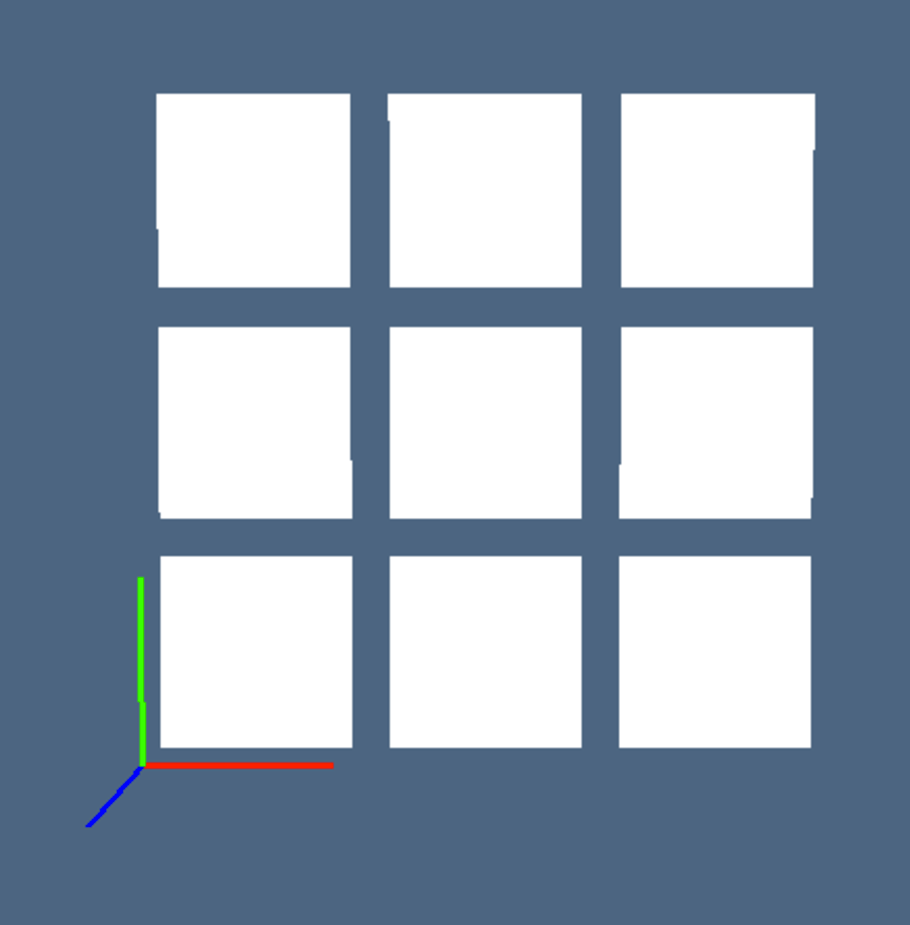
\includegraphics[width=0.458\linewidth]{images/grid2D} 
   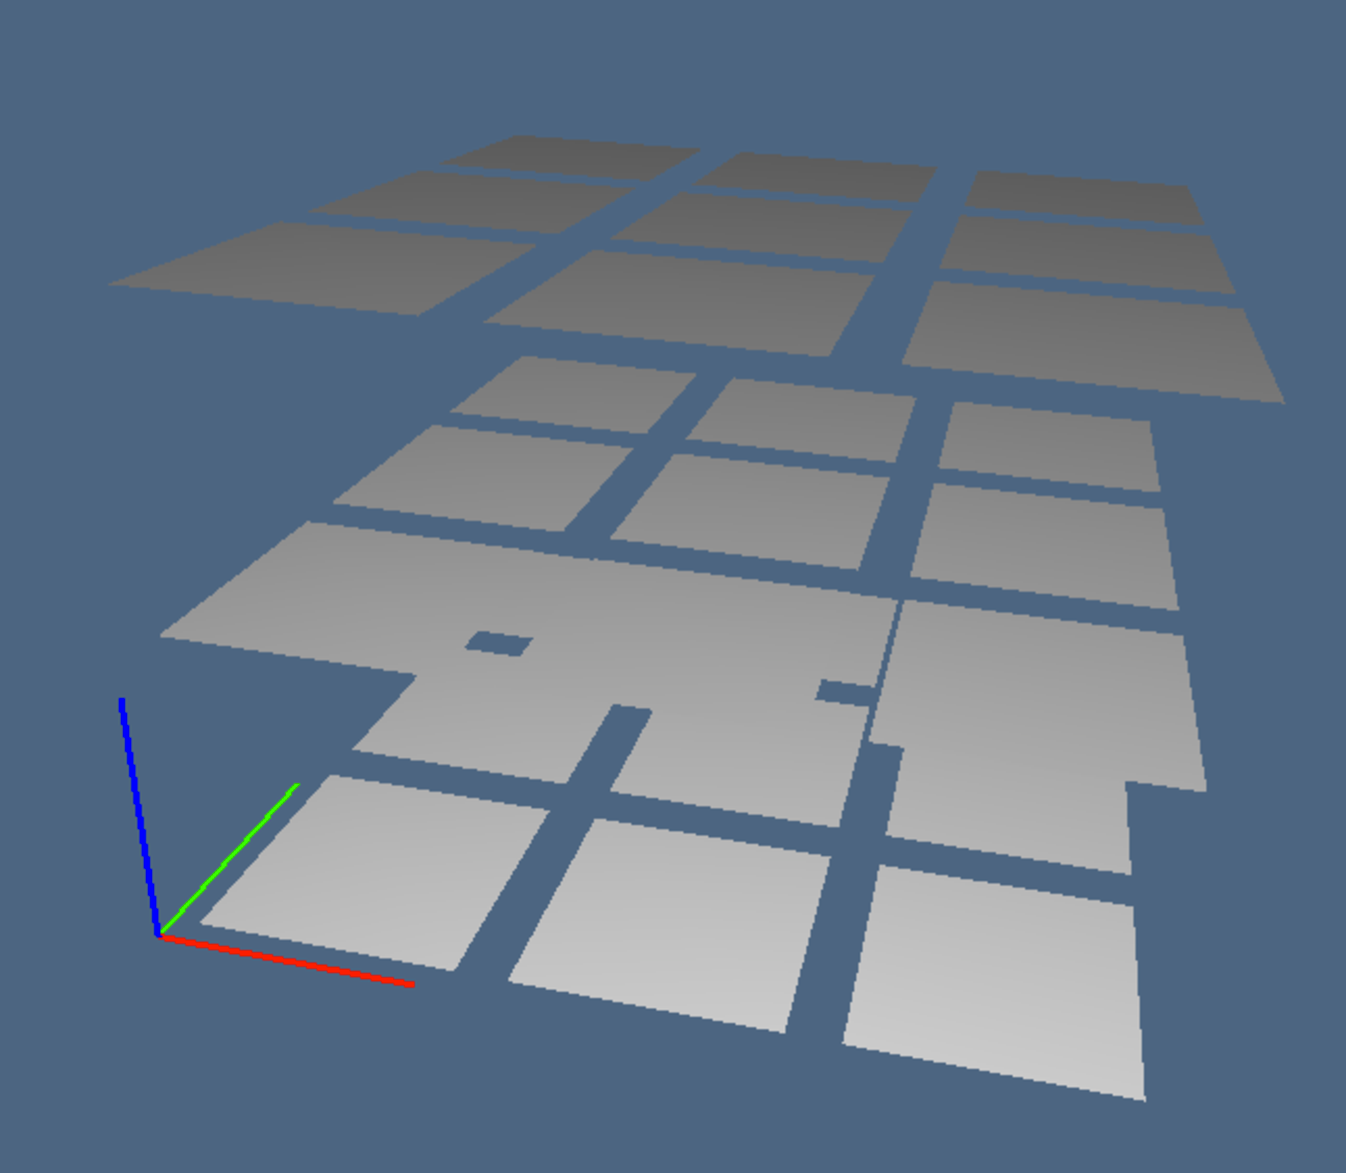
\includegraphics[width=0.532\linewidth]{images/grid3D} 
   \caption{Exploded views of models \texttt{grid2D} and \texttt{grid3D}.}
   \label{fig:firstgrid23D}
\end{figure}

Notice that \texttt{grid2D}, generated by product of two 1-complexes, is \emph{solid} in $\E^2$, whereas \texttt{grid3D} shown in Figure~\ref{fig:firstgrid23D}b, generated by product of two 1-complexes and one 0-complex, is two-dimensional and embedded in $\E^3$.

%-------------------------------------------------------------------------------
\begin{flushleft} \small \label{scrap8}
\protect\makebox[0ex][r]{\NWtarget{nuweb6b}{\rule{0ex}{0ex}}\hspace{1em}}$\langle\,$Example of cuboidal grid of dimensions $(2,3)$\nobreak\ {\footnotesize 6b}$\,\rangle\equiv$
\vspace{-1ex}
\begin{list}{}{} \item
\mbox{}\verb@v1, c1 = [[0.],[1.],[2.],[3.]],[[0,1],[1,2],[2,3]]@\\
\mbox{}\verb@v0, c0 = [[0.],[1.],[2.]], [[0],[1],[2]]@\\
\mbox{}\verb@vertGrid = larVertProd([v1, v1, v0])@\\
\mbox{}\verb@cellGrid = larCellProd([c1, c1, c0])@\\
\mbox{}\verb@grid3D = vertGrid,cellGrid@\\
\mbox{}\verb@VIEW(EXPLODE(1.2,1.2,1.2)(MKPOLS(grid3D)))@\\
\mbox{}\verb@@{\NWsep}
\end{list}
\vspace{-1ex}
\footnotesize\addtolength{\baselineskip}{-1ex}
\begin{list}{}{\setlength{\itemsep}{-\parsep}\setlength{\itemindent}{-\leftmargin}}
\item {\NWtxtMacroNoRef}.
\end{list}
\end{flushleft}
%-------------------------------------------------------------------------------

\paragraph{Cartesian product of 0/1-complexes}
Here, the input is given by the array \texttt{cellLists} of lists of cells of the argument complexes. Hence, the \texttt{shapes} variable contains the (list of) numbers $m_0, m_1, ...$ of cells in each argument complex, and the \texttt{indices} variable (generated by Cartesian product) collects the whole set $M_0 \times M_1 \times \cdots$ of 0-based multi-indices corresponding to the cells of the output complex, with $M_k = \{0,1,...,m_{k}-1\}$.

The \texttt{jointCells} variable is used to contain the list of outputs of Cartesian products of \texttt{cells} corresponding to every \texttt{index} in \texttt{indices}.

%-------------------------------------------------------------------------------
\begin{flushleft} \small \label{scrap9}
\protect\makebox[0ex][r]{\NWtarget{nuweb7}{\rule{0ex}{0ex}}\hspace{1em}}$\langle\,$Generation of grid cells\nobreak\ {\footnotesize 7}$\,\rangle\equiv$
\vspace{-1ex}
\begin{list}{}{} \item
\mbox{}\verb@def larCellProd(cellLists):@\\
\mbox{}\verb@    shapes = [len(item) for item in cellLists]@\\
\mbox{}\verb@    indices = CART([range(shape) for shape in shapes])@\\
\mbox{}\verb@    jointCells = [CART([cells[k] for k,cells in zip(index,cellLists)])@\\
\mbox{}\verb@                  for index in indices]@\\
\mbox{}\verb@    convert = index2addr([ shape+1 if (len(cellLists[k][0]) > 1) else shape@\\
\mbox{}\verb@                             for k,shape in enumerate(shapes) ])@\\
\mbox{}\verb@    return [AA(convert)(cell) for cell in jointCells]@\\
\mbox{}\verb@@{\NWsep}
\end{list}
\vspace{-1ex}
\footnotesize\addtolength{\baselineskip}{-1ex}
\begin{list}{}{\setlength{\itemsep}{-\parsep}\setlength{\itemindent}{-\leftmargin}}
\item \NWtxtMacroRefIn\ \NWlink{nuweb16a}{16a}.
\end{list}
\end{flushleft}
%-------------------------------------------------------------------------------

With reference to the evaluation of the expression \texttt{larCellProd([c1,c1])}, where \texttt{c1} is the LAR representation of a 1-complex with 3 cells, defined by 4 vertices (0-cells), we have the  trace given below.
Of course, the function invocation returns the list of cells of the topological product of the input complexes, each one expressed as a list of vertices of the Cartesian product of the corresponding component vertices. The partially evaluated function \texttt{index2addr0}, stored in the \texttt{convert} variable, is used to execute the mapping, for each output \texttt{cell} in \texttt{jointCells}, from vertex multi-indices to their linear storage address. The mindful reader should notice that the number of generated cells is always equal to the product of terms in \texttt{shape}, in turn equal to the number of elements in \texttt{indices} and in \texttt{jointCells}. In this case we have $|\texttt{larCellProd([c1,c1])}| = 3\times 3=9$.

%-------------------------------------------------------------------------------
\begin{flushleft} \small \label{scrap10}
\protect\makebox[0ex][r]{\NWtarget{nuweb8}{\rule{0ex}{0ex}}\hspace{1em}}$\langle\,$Tracing the evaluation of expression ``\texttt{larCellProd([c1,c1])}''\nobreak\ {\footnotesize 8}$\,\rangle\equiv$
\vspace{-1ex}
\begin{list}{}{} \item
\mbox{}\verb@c1 = [[0,1], [1,2], [2,3]]@\\
\mbox{}\verb@cellLists = [[[0,1], [1,2], [2,3]], [[0,1], [1,2], [2,3]]]@\\
\mbox{}\verb@shapes = [3,3]@\\
\mbox{}\verb@indices = [[0,0], [0,1], [0,2], [1,0], [1,1], [1,2], [2,0], [2,1], [2,2]]@\\
\mbox{}\verb@jointCells = [@\\
\mbox{}\verb@ [[0,0], [0,1], [1,0], [1,1]],@\\
\mbox{}\verb@ [[0,1], [0,2], [1,1], [1,2]],@\\
\mbox{}\verb@ [[0,2], [0,3], [1,2], [1,3]],@\\
\mbox{}\verb@ [[1,0], [1,1], [2,0], [2,1]],@\\
\mbox{}\verb@ [[1,1], [1,2], [2,1], [2,2]],@\\
\mbox{}\verb@ [[1,2], [1,3], [2,2], [2,3]],@\\
\mbox{}\verb@ [[2,0], [2,1], [3,0], [3,1]],@\\
\mbox{}\verb@ [[2,1], [2,2], [3,1], [3,2]],@\\
\mbox{}\verb@ [[2,2], [2,3], [3,2], [3,3]]]@\\
\mbox{}\verb@convert = <function index2address0>@\\
\mbox{}\verb@return [@\\
\mbox{}\verb@ [0,1,4,5],@\\
\mbox{}\verb@ [1,2,5,6],@\\
\mbox{}\verb@ [2,3,6,7],@\\
\mbox{}\verb@ [4,5,8,9],@\\
\mbox{}\verb@ [5,6,9,10],@\\
\mbox{}\verb@ [6,7,10,11],@\\
\mbox{}\verb@ [8,9,12,13],@\\
\mbox{}\verb@ [9,10,13,14],@\\
\mbox{}\verb@ [10,11,14,15]]@\\
\mbox{}\verb@@{\NWsep}
\end{list}
\vspace{-1ex}
\footnotesize\addtolength{\baselineskip}{-1ex}
\begin{list}{}{\setlength{\itemsep}{-\parsep}\setlength{\itemindent}{-\leftmargin}}
\item {\NWtxtMacroNoRef}.
\end{list}
\end{flushleft}
%-------------------------------------------------------------------------------


\subsection{Lower-dimensional grid skeletons}

In order to compute the $d$-skeletons of a $n$-dimensional cuboidal ``grid'' complex, with $0\leq d\leq n$, let us start by remarking a similarity with the generation of the boolean representation of numbers between 0 and $2^n -1$, generated as a list of strings by the \texttt{binaryRange} function, given in Section~\ref{sec:binaryRange}.

The binary representations of such numbers are in fact filtered according to the number of their ones in Section~\ref{sec:filterByOrder}, and used to generate the distinct components of different order skeletons of the assembled grid complexes in Section~\ref{sec:assembly}.

\subsubsection{Generation of skeleton components}
\label{sec:binaryRange}

The \texttt{binaryRange} function, applied to an integer $n$, returns the string representation of all binary numerals between 0 and $2^n -1$. All the strings have the same length $n$. The bits in each strings will be used to select between either a 0- or a 1-dimensional complex as generator (via a Cartesian product of complexes) of a component of an embedded grid skeleton of proper intrinsic dimension.

%-------------------------------------------------------------------------------
\begin{flushleft} \small \label{scrap11}
\protect\makebox[0ex][r]{\NWtarget{nuweb9a}{\rule{0ex}{0ex}}\hspace{1em}}$\langle\,$Enumeration of binary ranges of given order\nobreak\ {\footnotesize 9a}$\,\rangle\equiv$
\vspace{-1ex}
\begin{list}{}{} \item
\mbox{}\verb@def binaryRange(n):@\\
\mbox{}\verb@    return [('{0:0'+str(n)+'b}').format(k) for k in range(2**n)]@\\
\mbox{}\verb@@{\NWsep}
\end{list}
\vspace{-1ex}
\footnotesize\addtolength{\baselineskip}{-1ex}
\begin{list}{}{\setlength{\itemsep}{-\parsep}\setlength{\itemindent}{-\leftmargin}}
\item \NWtxtMacroRefIn\ \NWlink{nuweb16a}{16a}.
\end{list}
\end{flushleft}
%-------------------------------------------------------------------------------

\paragraph{Examples of generation of bit strings}
Below we show the outputs returned by application of the \texttt{binaryRange} function to the first 4 integers.
%-------------------------------------------------------------------------------
\begin{flushleft} \small \label{scrap12}
\protect\makebox[0ex][r]{\NWtarget{nuweb9b}{\rule{0ex}{0ex}}\hspace{1em}}$\langle\,$Binary range examples\nobreak\ {\footnotesize 9b}$\,\rangle\equiv$
\vspace{-1ex}
\begin{list}{}{} \item
\mbox{}\verb@>>> print binaryRange(4),@\\
\mbox{}\verb@['0000', '0001', '0010', '0011', '0100', '0101', '0110', '0111', @\\
\mbox{}\verb@ '1000', '1001', '1010', '1011', '1100', '1101', '1110', '1111']@\\
\mbox{}\verb@>>> print binaryRange(3),@\\
\mbox{}\verb@['000', '001', '010', '011', '100', '101', '110', '111']@\\
\mbox{}\verb@>>> print binaryRange(2),@\\
\mbox{}\verb@['00', '01', '10', '11']@\\
\mbox{}\verb@>>> print binaryRange(1),@\\
\mbox{}\verb@['0', '1']@\\
\mbox{}\verb@@{\NWsep}
\end{list}
\vspace{-1ex}
\footnotesize\addtolength{\baselineskip}{-1ex}
\begin{list}{}{\setlength{\itemsep}{-\parsep}\setlength{\itemindent}{-\leftmargin}}
\item {\NWtxtMacroNoRef}.
\end{list}
\end{flushleft}
%-------------------------------------------------------------------------------

\subsubsection{Filtering grid skeleton components}
\label{sec:filterByOrder}

The function \texttt{filterByOrder} is used to partition the previous binary strings into $n+1$ subsets, such that the bits into each string sum to the same number, ranging from 0 to $n$ included, respectively.

%-------------------------------------------------------------------------------
\begin{flushleft} \small \label{scrap13}
\protect\makebox[0ex][r]{\NWtarget{nuweb9c}{\rule{0ex}{0ex}}\hspace{1em}}$\langle\,$Filtering binary ranges by order\nobreak\ {\footnotesize 9c}$\,\rangle\equiv$
\vspace{-1ex}
\begin{list}{}{} \item
\mbox{}\verb@def filterByOrder(n):@\\
\mbox{}\verb@    terms = [AA(int)(list(term)) for term in binaryRange(n)]@\\
\mbox{}\verb@    return [[term for term in terms if sum(term) == k] for k in range(n+1)]@\\
\mbox{}\verb@@{\NWsep}
\end{list}
\vspace{-1ex}
\footnotesize\addtolength{\baselineskip}{-1ex}
\begin{list}{}{\setlength{\itemsep}{-\parsep}\setlength{\itemindent}{-\leftmargin}}
\item \NWtxtMacroRefIn\ \NWlink{nuweb16a}{16a}.
\end{list}
\end{flushleft}
%-------------------------------------------------------------------------------

\paragraph{Examples of bit lists filtering}
Some examples of application of the \texttt{filterByOrder} function to the first few integers are shown below.
Of course, the number of elements in each class (i.e.~in each returned list) is ${n \choose d}$, and the total number of elements for each fixed $n$ is $\sum_{d=0}^n {n \choose d} = 2^n$.

%-------------------------------------------------------------------------------
\begin{flushleft} \small \label{scrap14}
\protect\makebox[0ex][r]{\NWtarget{nuweb10a}{\rule{0ex}{0ex}}\hspace{1em}}$\langle\,$Skeleton component examples\nobreak\ {\footnotesize 10a}$\,\rangle\equiv$
\vspace{-1ex}
\begin{list}{}{} \item
\mbox{}\verb@>>> filterByOrder(4)@\\
\mbox{}\verb@[[[0,0,0,0]],@\\
\mbox{}\verb@ [[0,0,0,1], [0,0,1,0], [0,1,0,0], [1,0,0,0]],@\\
\mbox{}\verb@ [[0,0,1,1], [0,1,0,1], [0,1,1,0], [1,0,0,1], [1,0,1,0], [1,1,0,0]],@\\
\mbox{}\verb@ [[0,1,1,1], [1,0,1,1], [1,1,0,1], [1,1,1,0]],@\\
\mbox{}\verb@ [[1,1,1,1]]]@\\
\mbox{}\verb@>>> filterByOrder(3)@\\
\mbox{}\verb@[[[0,0,0]],@\\
\mbox{}\verb@ [[0,0,1], [0,1,0], [1,0,0]],@\\
\mbox{}\verb@ [[0,1,1], [1,0,1], [1,1,0]],@\\
\mbox{}\verb@ [[1,1,1]]]@\\
\mbox{}\verb@>>> filterByOrder(2)@\\
\mbox{}\verb@[[[0,0]], [[0,1], [1,0]], [[1,1]]]@\\
\mbox{}\verb@>>> filterByOrder(1)@\\
\mbox{}\verb@[[[0]], [[1]]]@\\
\mbox{}\verb@@{\NWsep}
\end{list}
\vspace{-1ex}
\footnotesize\addtolength{\baselineskip}{-1ex}
\begin{list}{}{\setlength{\itemsep}{-\parsep}\setlength{\itemindent}{-\leftmargin}}
\item {\NWtxtMacroNoRef}.
\end{list}
\end{flushleft}
%-------------------------------------------------------------------------------


\subsubsection{Assembling grid skeleton components}
\label{sec:assembly}

We are now finally able to generate the various subsets of cells of a $d$-dimensional cuboidal grid skeleton, produced respectively by the expression \texttt{larCellProd(cellLists)} for every permutation of 0- and 1-complexes, according to the partition classes of permtation of $n$ bits previously produced. To understand why this assembling step of cells is necessary, the reader should look at Figure~\ref{fig:sleletons}, where three subsets of 2-cells of the 2-skeleton, respectively generated by the bit dispositions \texttt{[[0,1,1], [1,0,1], [1,1,0]]}, are separately displayed.
Notice also that, whereas the dimension $n$ of the embedding space is implicittly provided by the \texttt{length} of the \texttt{shape} parameter, the intrinsic dimension $d$ of the skeleton to be produced must be given explicitly.

\begin{figure}[htbp] %  figure placement: here, top, bottom, or page
   \centering
   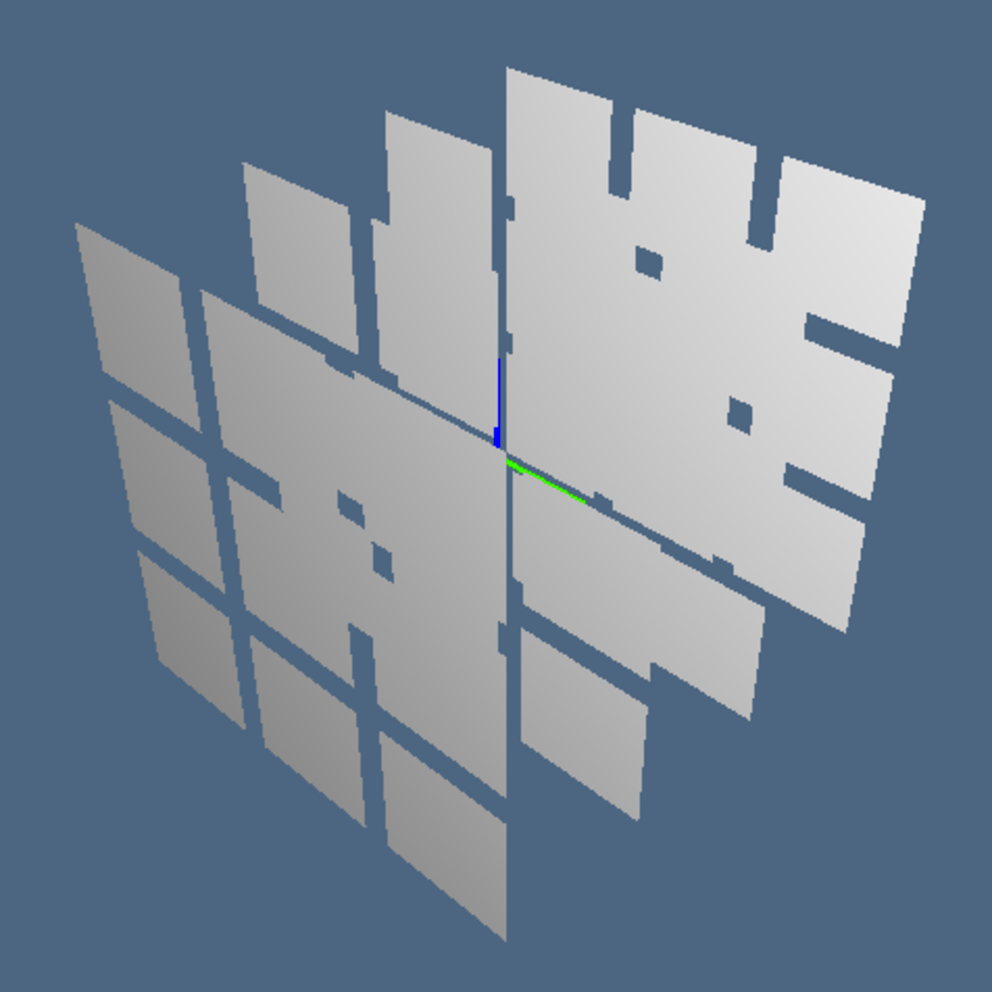
\includegraphics[height=0.245\linewidth,width=0.242\linewidth]{images/skel2a} 
   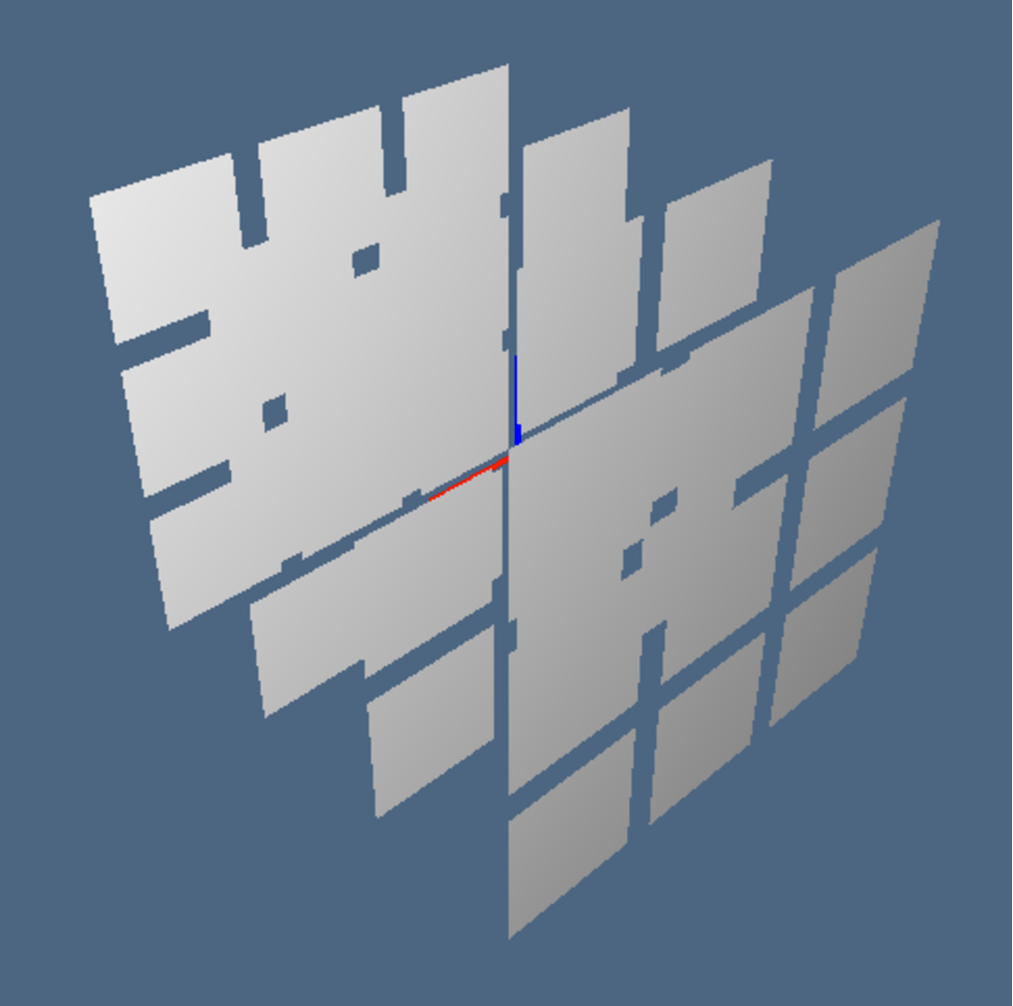
\includegraphics[height=0.245\linewidth,width=0.242\linewidth]{images/skel2b} 
   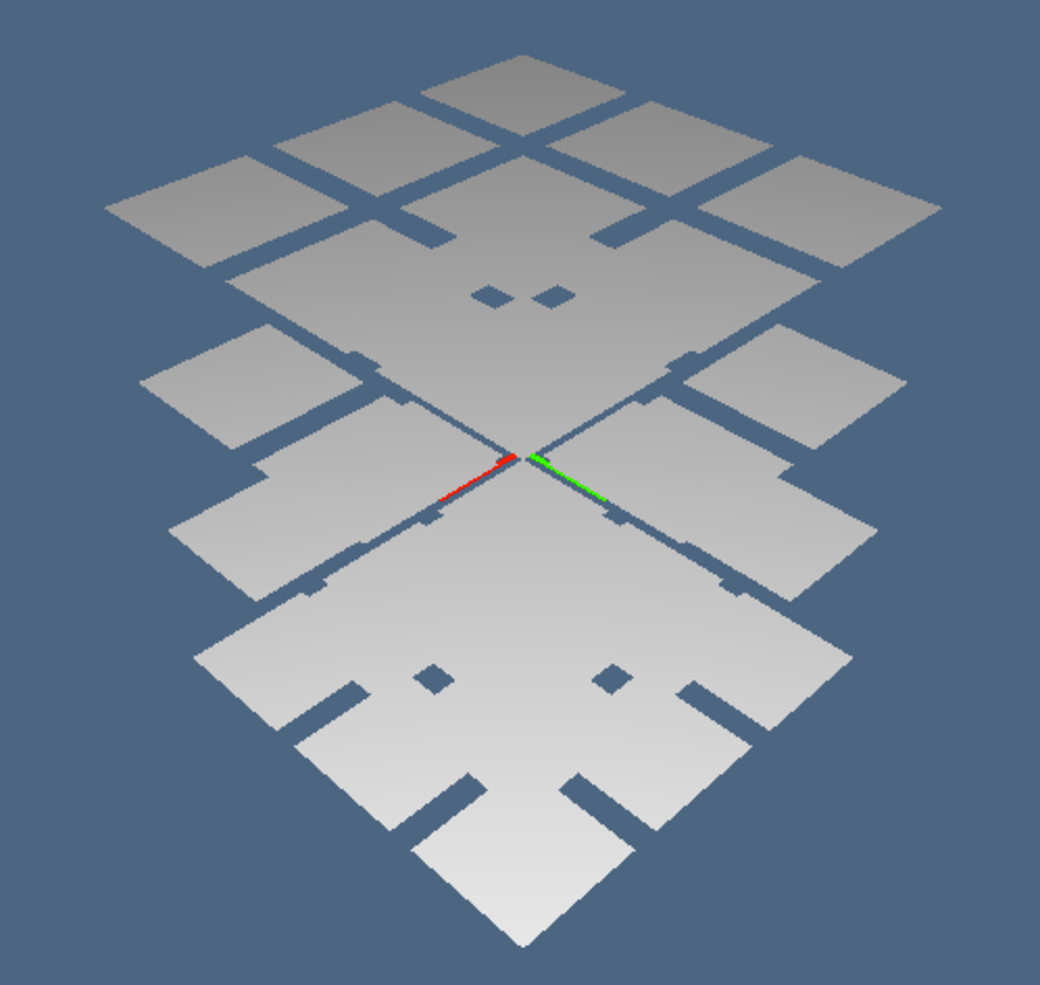
\includegraphics[height=0.245\linewidth,width=0.242\linewidth]{images/skel2c} 
   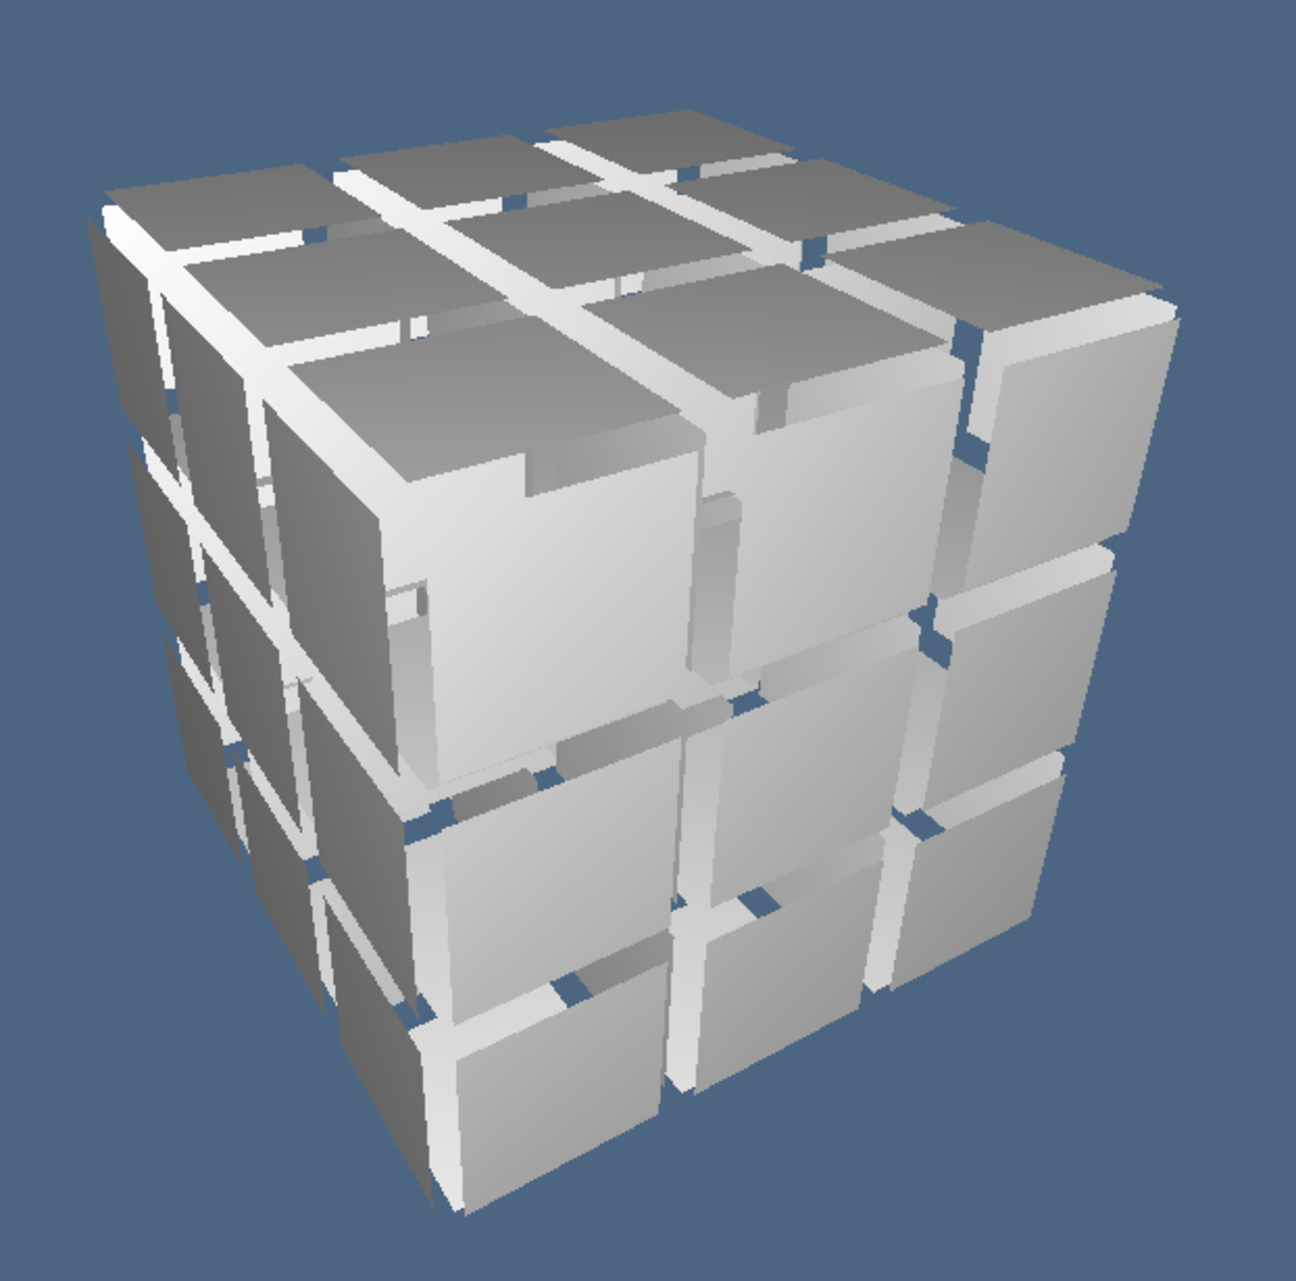
\includegraphics[height=0.245\linewidth,width=0.242\linewidth]{images/skel2} 
   \caption{(a,b,c) Exploded views of subsets (orthogonal to coordinate axes) of 2-cells of a 2-skeleton grid; (d) their assembled set.}
   \label{fig:sleletons}
\end{figure}

%-------------------------------------------------------------------------------
\begin{flushleft} \small \label{scrap15}
\protect\makebox[0ex][r]{\NWtarget{nuweb10b}{\rule{0ex}{0ex}}\hspace{1em}}$\langle\,$Assembling grid skeletons\nobreak\ {\footnotesize 10b}$\,\rangle\equiv$
\vspace{-1ex}
\begin{list}{}{} \item
\mbox{}\verb@def larGridSkeleton(shape):@\\
\mbox{}\verb@    n = len(shape)@\\
\mbox{}\verb@    def larGridSkeleton0(d):@\\
\mbox{}\verb@        components = filterByOrder(n)[d]@\\
\mbox{}\verb@        componentCellLists = [AA(APPLY)(zip( AA(larGrid)(shape),(component) ))@\\
\mbox{}\verb@                              for component in components]@\\
\mbox{}\verb@        return CAT([ larCellProd(cellLists)  for cellLists in componentCellLists ])@\\
\mbox{}\verb@    return larGridSkeleton0@\\
\mbox{}\verb@@{\NWsep}
\end{list}
\vspace{-1ex}
\footnotesize\addtolength{\baselineskip}{-1ex}
\begin{list}{}{\setlength{\itemsep}{-\parsep}\setlength{\itemindent}{-\leftmargin}}
\item \NWtxtMacroRefIn\ \NWlink{nuweb16a}{16a}.
\end{list}
\end{flushleft}
%-------------------------------------------------------------------------------


\begin{figure}[htbp] %  figure placement: here, top, bottom, or page
   \centering
   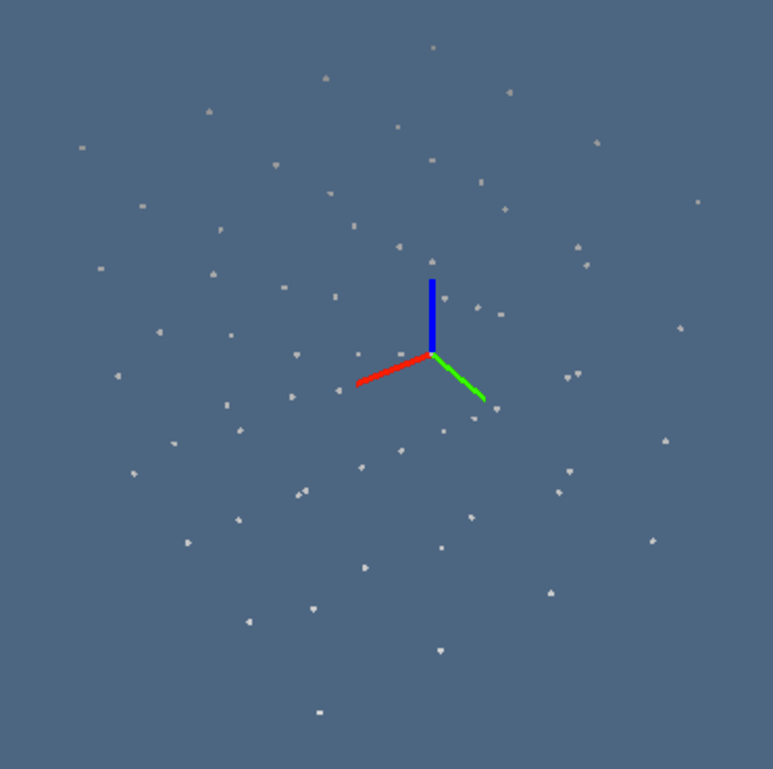
\includegraphics[height=0.245\linewidth,width=0.242\linewidth]{images/skel0} 
   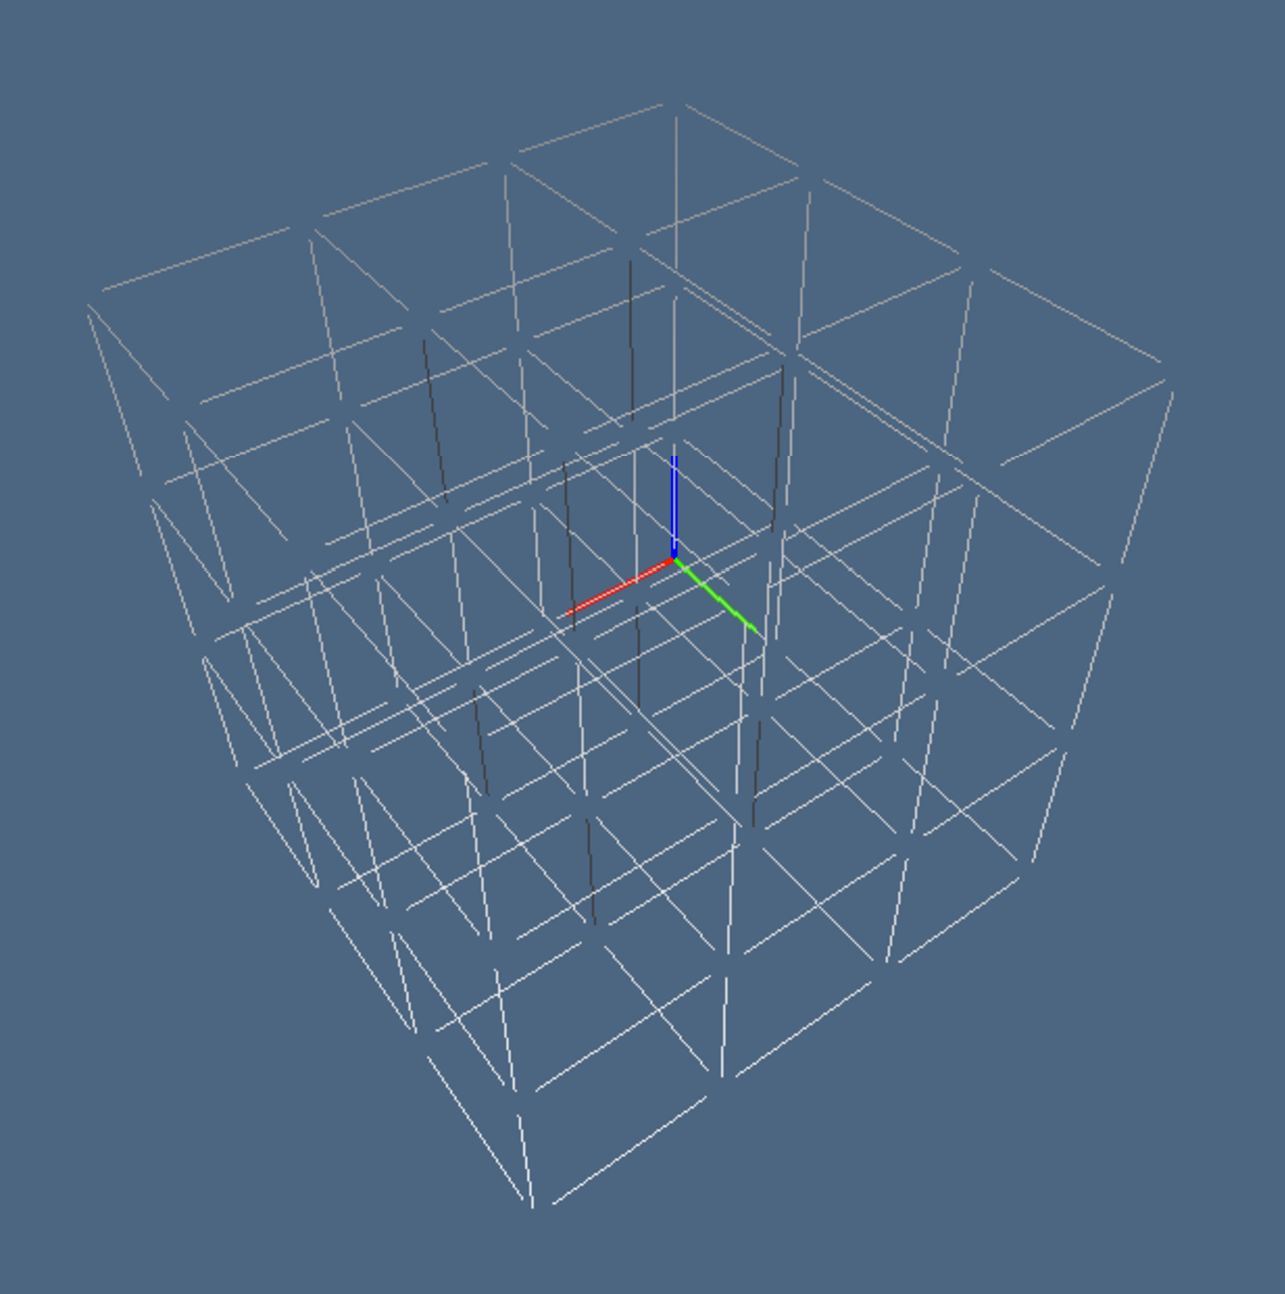
\includegraphics[height=0.245\linewidth,width=0.242\linewidth]{images/skel1} 
   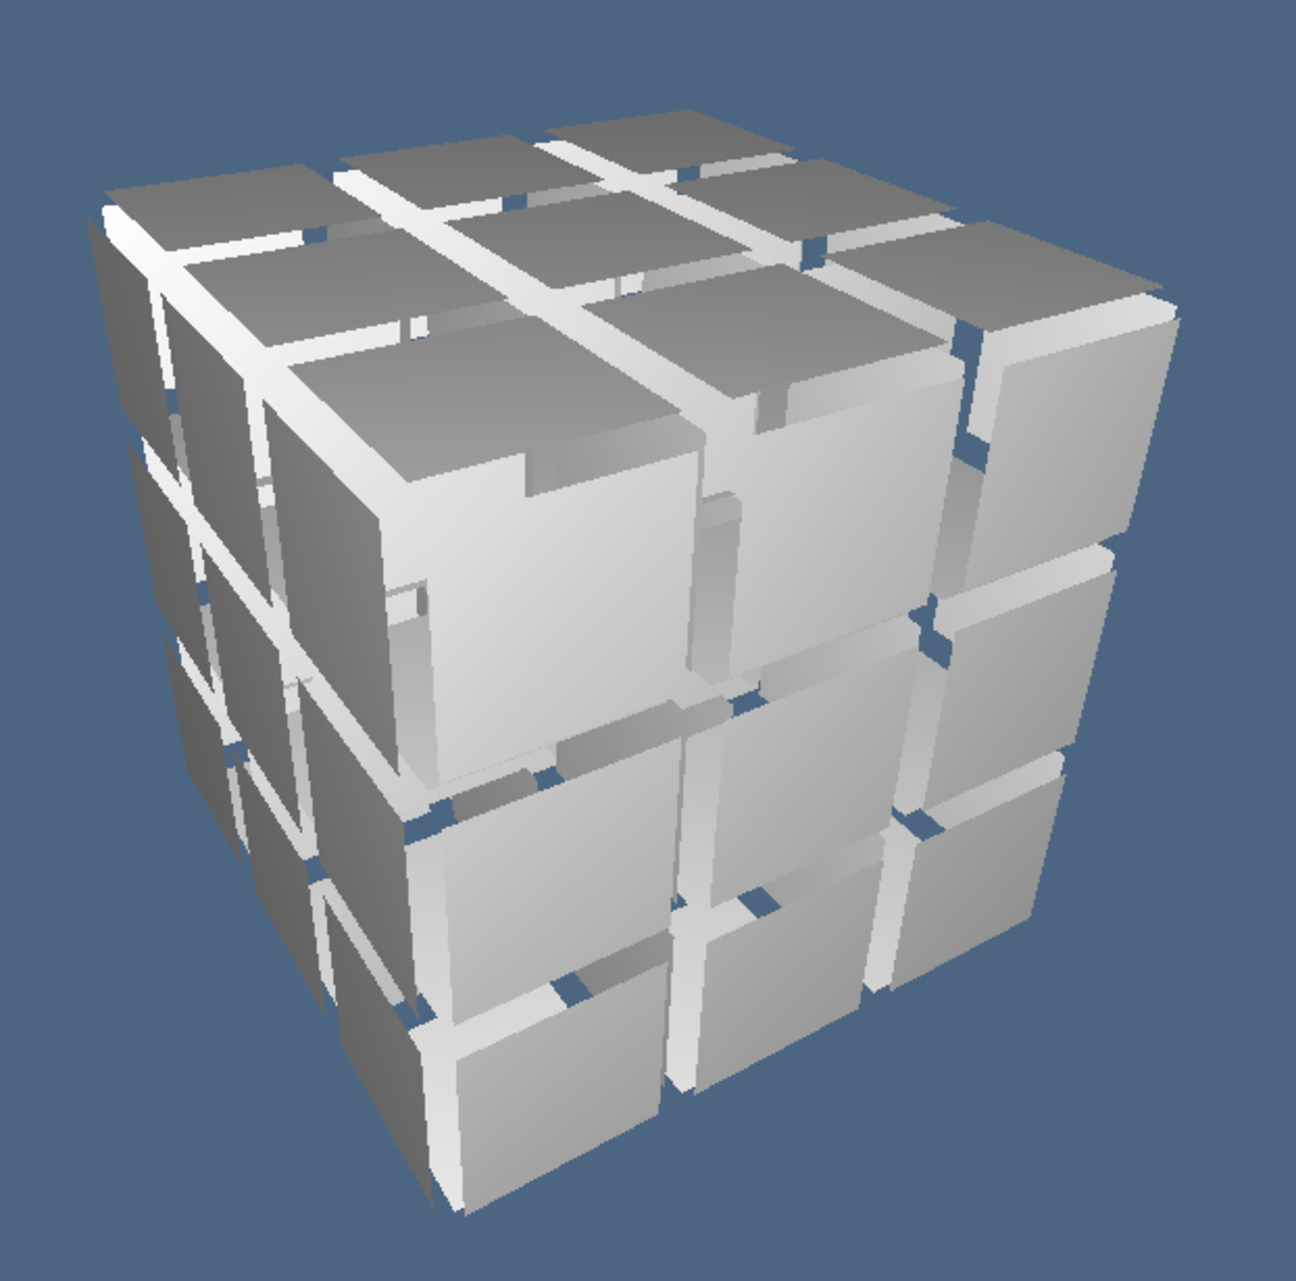
\includegraphics[height=0.245\linewidth,width=0.242\linewidth]{images/skel2} 
   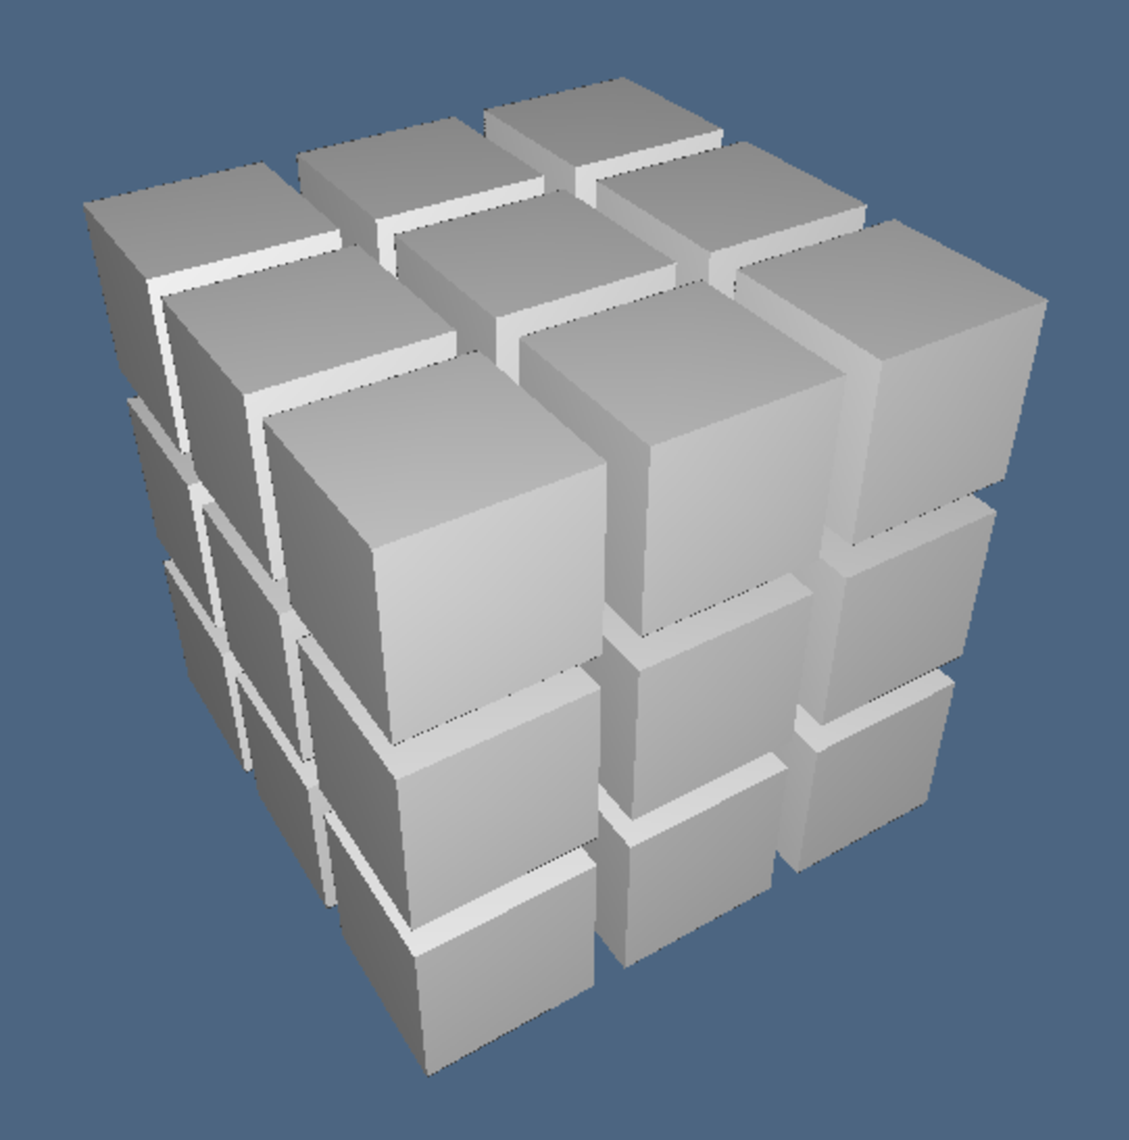
\includegraphics[height=0.245\linewidth,width=0.242\linewidth]{images/skel3} 
   \caption{Exploded views of 0-, 1-, 2-, and 3-dimensional skeletons.}
   \label{fig:grid23D}
\end{figure}

\subsection{Highest-level grid interface}

The highest-level user interface for (hyper)-cuboidal grid generation is given by the function \texttt{larCuboids}  applied to the \texttt{shape} parameter.  
For the sake of storage efficiency, the generated vertex coordinates are integer and 0-based in the lowest corner. The model may be properly scaled and/or translated \emph{a posteriori} when needed.

\paragraph{Generation of (hyper)-cuboidal grids}

The generated complex is always full-dimension, i.e.~\emph{solid}, and possibly includes the cells of all dimensions, depending on the Boolean value of the \texttt{full} parameter.
The grid's intrinsic dimension, as well as the dimension of its embedding space, are specified by the length of the \texttt{shape} parameter. See the examples in Figure~\ref{fig:grid23D}, but remember that the PLaSM visualiser always embed in 3D the displayed model. 

%-------------------------------------------------------------------------------
\begin{flushleft} \small \label{scrap16}
\protect\makebox[0ex][r]{\NWtarget{nuweb12a}{\rule{0ex}{0ex}}\hspace{1em}}$\langle\,$Multidimensional grid generation\nobreak\ {\footnotesize 12a}$\,\rangle\equiv$
\vspace{-1ex}
\begin{list}{}{} \item
\mbox{}\verb@def larImageVerts(shape):@\\
\mbox{}\verb@   def vertexDomain(n): @\\
\mbox{}\verb@      return [[k] for k in range(n)]@\\
\mbox{}\verb@   vertLists = [vertexDomain(k+1) for k in shape]@\\
\mbox{}\verb@   vertGrid = larVertProd(vertLists)@\\
\mbox{}\verb@   return vertGrid@\\
\mbox{}\verb@@\\
\mbox{}\verb@def larCuboids(shape, full=False):@\\
\mbox{}\verb@   vertGrid = larImageVerts(shape)@\\
\mbox{}\verb@   gridMap = larGridSkeleton(shape)@\\
\mbox{}\verb@   if not full: @\\
\mbox{}\verb@      cells = gridMap(len(shape))@\\
\mbox{}\verb@   else:@\\
\mbox{}\verb@      skeletonIds = range(len(shape)+1)@\\
\mbox{}\verb@      cells = CAT([ gridMap(id) for id in skeletonIds ])@\\
\mbox{}\verb@   return vertGrid, cells@\\
\mbox{}\verb@@{\NWsep}
\end{list}
\vspace{-1ex}
\footnotesize\addtolength{\baselineskip}{-1ex}
\begin{list}{}{\setlength{\itemsep}{-\parsep}\setlength{\itemindent}{-\leftmargin}}
\item \NWtxtMacroRefIn\ \NWlink{nuweb16a}{16a}.
\end{list}
\end{flushleft}
%-------------------------------------------------------------------------------

\paragraph{Multidimensional visualisation examples}
Visualisation examples of grid of dimension 1,2, and 3 are given below and are displayed  in Figure~\ref{fig:grid23D}. The same input pattern may be used for higher-dimensional grids (say, of dimension 4 and beyond), but to be visualised they should be carefully and properly projected in 3D.

%-------------------------------------------------------------------------------
\begin{flushleft} \small
\begin{minipage}{\linewidth} \label{scrap17}
\protect\makebox[0ex][r]{\NWtarget{nuweb12b}{\rule{0ex}{0ex}}\hspace{1em}}$\langle\,$Multidimensional visualisation examples\nobreak\ {\footnotesize 12b}$\,\rangle\equiv$
\vspace{-1ex}
\begin{list}{}{} \item
\mbox{}\verb@VIEW(EXPLODE(1.5,1.5,1.5)(MKPOLS(larCuboids([3],True))))@\\
\mbox{}\verb@VIEW(EXPLODE(1.5,1.5,1.5)(MKPOLS(larCuboids([3,2],True))))@\\
\mbox{}\verb@VIEW(EXPLODE(1.5,1.5,1.5)(MKPOLS(larCuboids([3,2,1],True))))@\\
\mbox{}\verb@@{\NWsep}
\end{list}
\vspace{-1ex}
\footnotesize\addtolength{\baselineskip}{-1ex}
\begin{list}{}{\setlength{\itemsep}{-\parsep}\setlength{\itemindent}{-\leftmargin}}
\item \NWtxtMacroRefIn\ \NWlink{nuweb16a}{16a}.
\end{list}
\end{minipage}\\[4ex]
\end{flushleft}
%-------------------------------------------------------------------------------

\begin{figure}[htbp] %  figure placement: here, top, bottom, or page
   \centering
   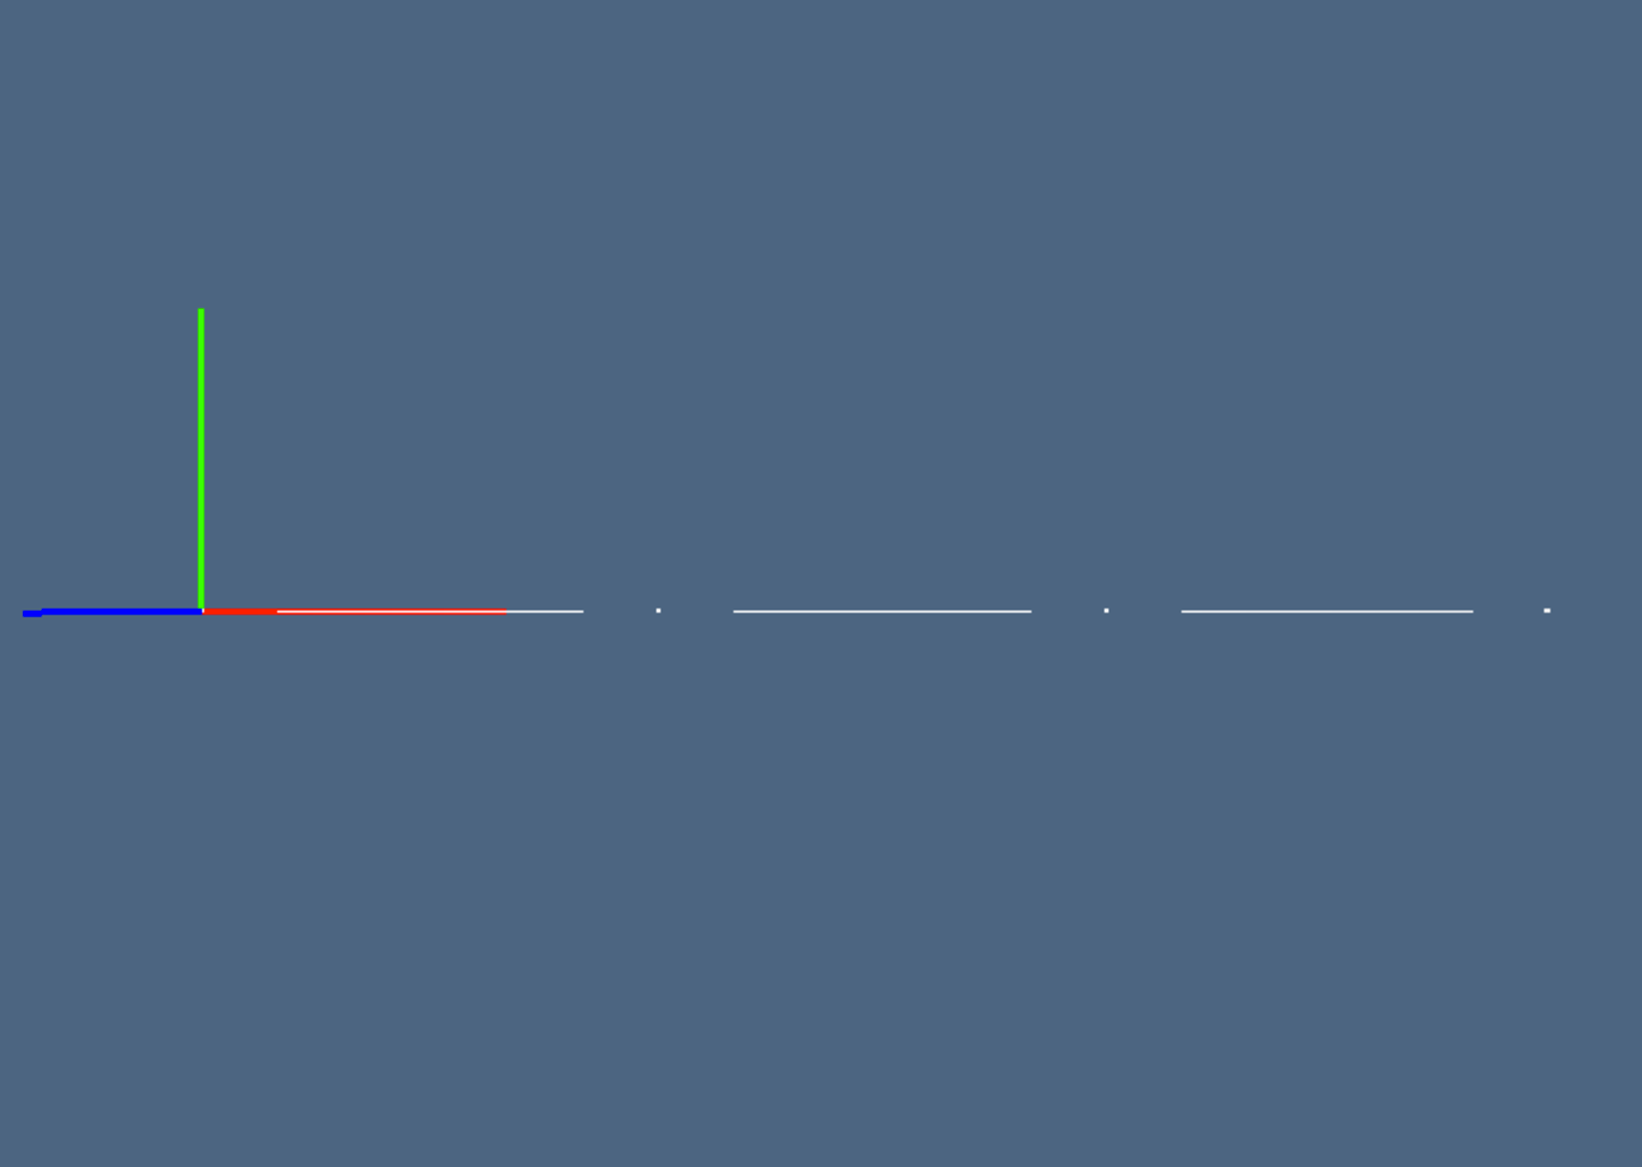
\includegraphics[width=0.313\linewidth]{images/complex3} 
   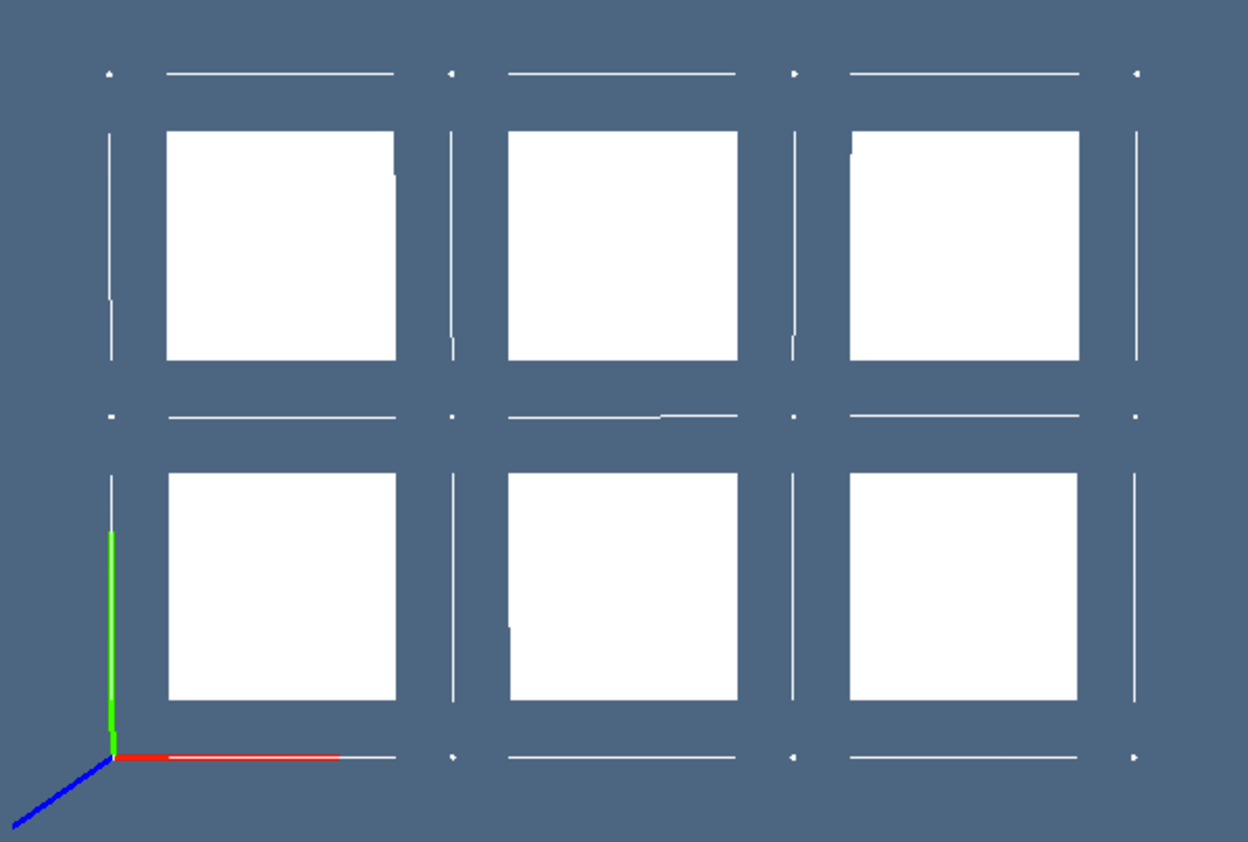
\includegraphics[width=0.33\linewidth]{images/complex32} 
   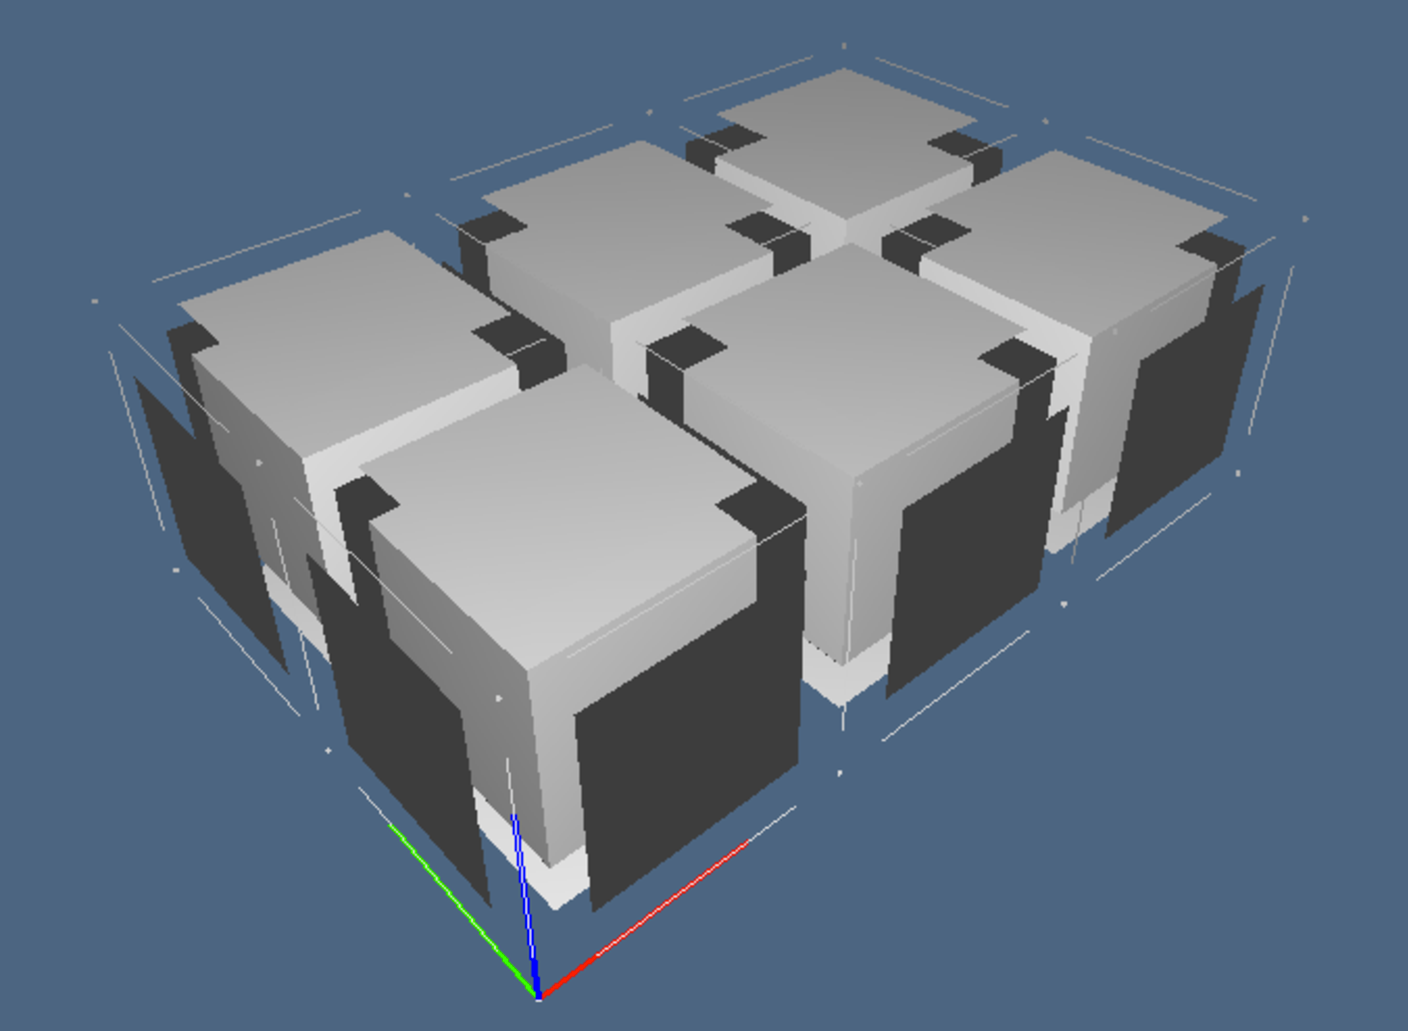
\includegraphics[width=0.305\linewidth]{images/complex321} 
   \caption{Exploded views of 1D, 2D, and 3D cellular complexes (including cells of dimension 0,1,2, and 3).}
   \label{fig:grid23D}
\end{figure}


\subsection{Chain of boundary operators}

As we know, a \emph{chain complex} is a sequence of (linear) chain spaces $C_k$ ($d\geq k\geq 0$) and a sequence
of boundary operators $\partial_k: C_k \to C_{k-1}$ ($d\geq k\geq 1$) between adjacent spaces (see Figure~\ref{fig:chainComplexMap}). In this section, we aim to generate the sequence of boundary matrices \texttt{CSR($[\partial_k]$)} ($1\leq k\leq d$).

\begin{figure}[htbp] %  figure placement: here, top, bottom, or page
   \centering
   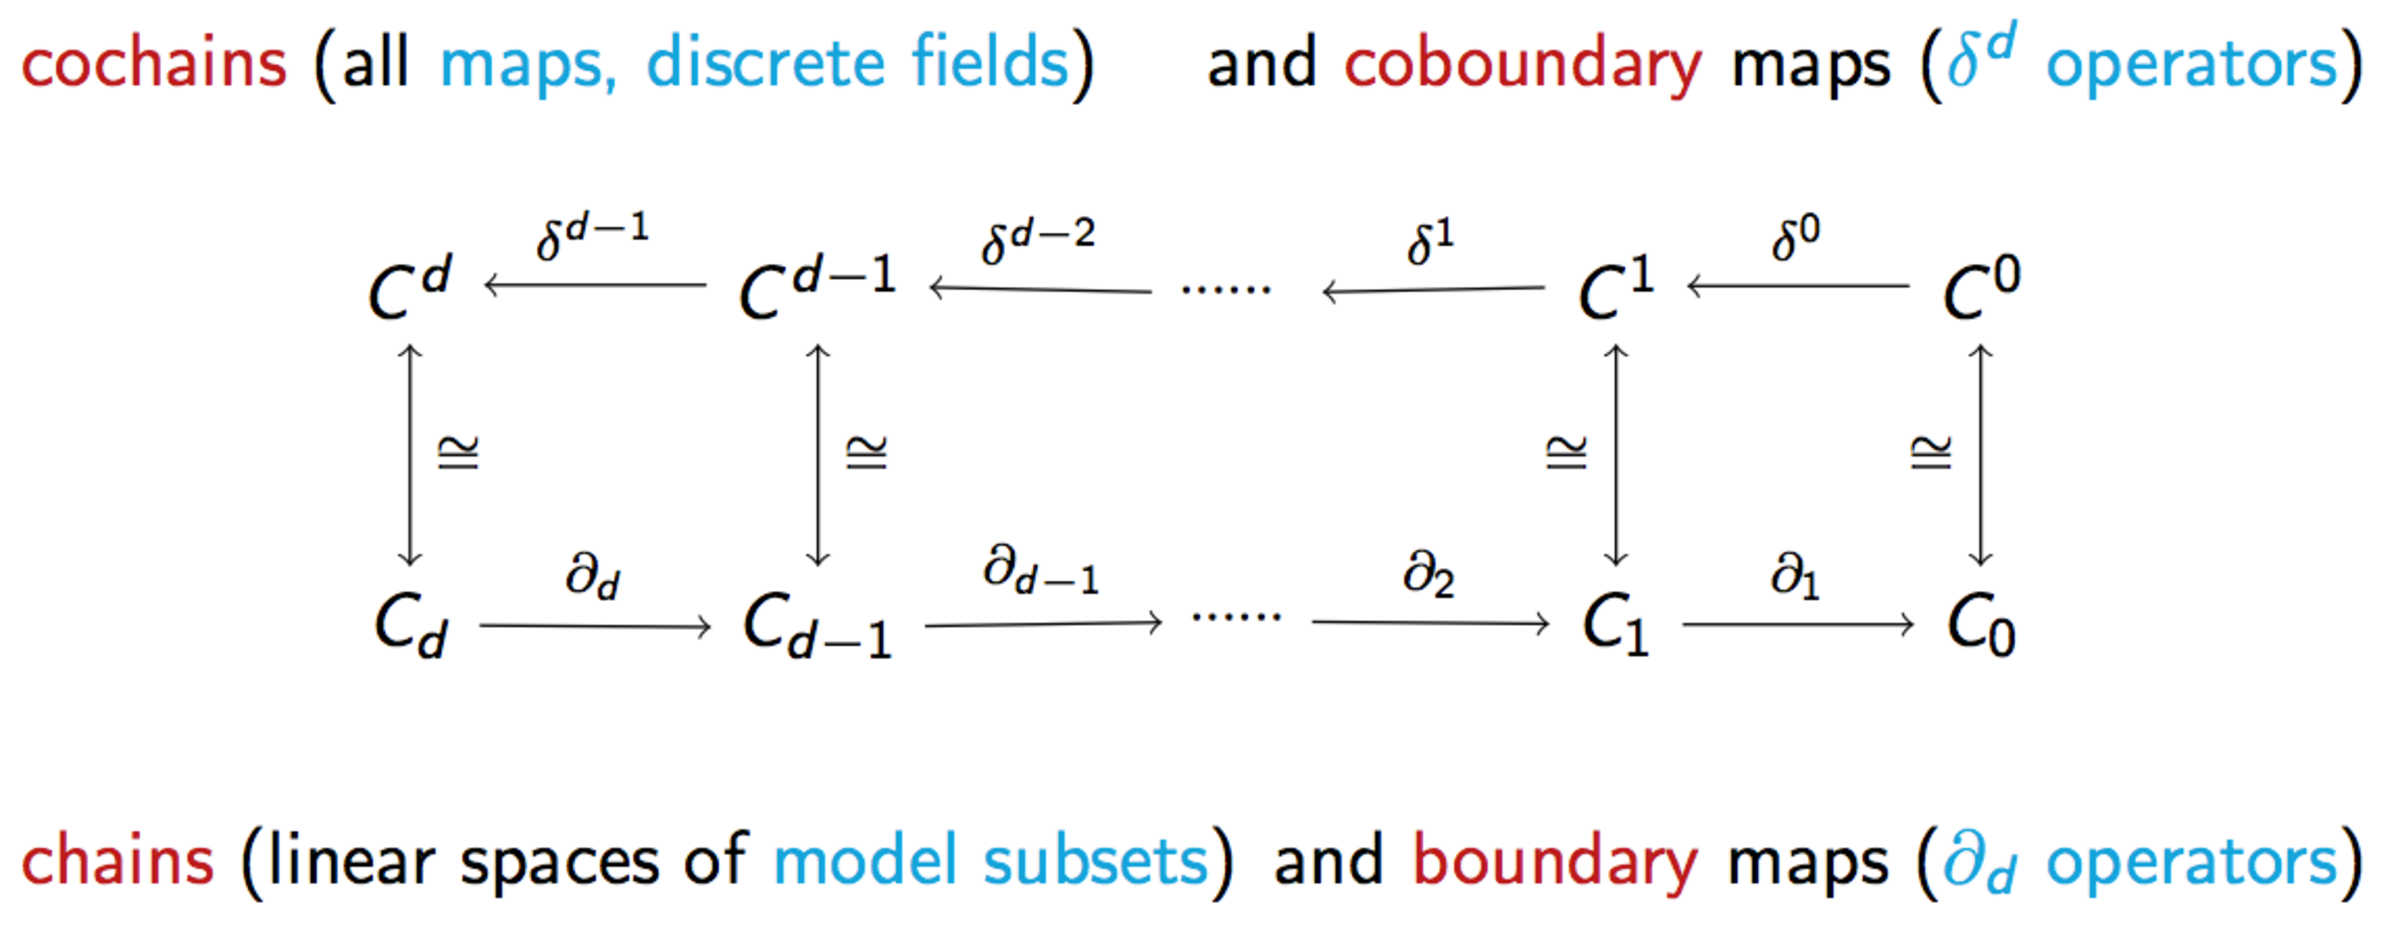
\includegraphics[width=0.8\linewidth]{images/chainComplexMap} 
   \caption{Chain and cochain complexes.}
   \label{fig:chainComplexMap}
\end{figure}

\paragraph{Cuboidal skeletons}
A list of \texttt{BRC} characteristic matrices of cellular $k$-complexes ($0\leq k\leq d$) with dimension $d$, where $d={}$\texttt{len(shape)}, is returned by the function \texttt{gridSkeletons} in the macro below, where the input is given by the \emph{shape} of the grid, i.e.~by the list of cell items in each coordinate direction. Some simple test examples of skeletons of cuboidal complexes are also printed when the \texttt{largrid} module run as the \texttt{main}. Just notice that the number of returned $d$-cells is equal to \texttt{PROD(shape)}.

%-------------------------------------------------------------------------------
\begin{flushleft} \small \label{scrap18}
\protect\makebox[0ex][r]{\NWtarget{nuweb13}{\rule{0ex}{0ex}}\hspace{1em}}$\langle\,$Multidimensional grid skeletons\nobreak\ {\footnotesize 13}$\,\rangle\equiv$
\vspace{-1ex}
\begin{list}{}{} \item
\mbox{}\verb@def gridSkeletons(shape):@\\
\mbox{}\verb@   gridMap = larGridSkeleton(shape)@\\
\mbox{}\verb@   skeletonIds = range(len(shape)+1)@\\
\mbox{}\verb@   skeletons = [ gridMap(id) for id in skeletonIds ]@\\
\mbox{}\verb@   return skeletons@\\
\mbox{}\verb@   @\\
\mbox{}\verb@if __name__=="__main__":@\\
\mbox{}\verb@   print "\ngridSkeletons([3]) =\n", gridSkeletons([3])@\\
\mbox{}\verb@   print "\ngridSkeletons([3,2]) =\n", gridSkeletons([3,2])@\\
\mbox{}\verb@   print "\ngridSkeletons([3,2,1]) =\n", gridSkeletons([3,2,1])@\\
\mbox{}\verb@@{\NWsep}
\end{list}
\vspace{-1ex}
\footnotesize\addtolength{\baselineskip}{-1ex}
\begin{list}{}{\setlength{\itemsep}{-\parsep}\setlength{\itemindent}{-\leftmargin}}
\item \NWtxtMacroRefIn\ \NWlink{nuweb16a}{16a}.
\end{list}
\end{flushleft}
%-------------------------------------------------------------------------------

\paragraph{Boundary complex of a cuboidal grid}
The list of boundary matrices \texttt{CSR($[\partial_k]$)} ($1\leq k\leq d$) is returned by the function
\texttt{gridBoundaryMatrices}.

%-------------------------------------------------------------------------------
\begin{flushleft} \small \label{scrap19}
\protect\makebox[0ex][r]{\NWtarget{nuweb14}{\rule{0ex}{0ex}}\hspace{1em}}$\langle\,$Generation of grid boundary complex\nobreak\ {\footnotesize 14}$\,\rangle\equiv$
\vspace{-1ex}
\begin{list}{}{} \item
\mbox{}\verb@def gridBoundaryMatrices(shape):@\\
\mbox{}\verb@   skeletons = gridSkeletons(shape)@\\
\mbox{}\verb@   boundaryMatrices = [boundary(skeletons[k+1],faces) @\\
\mbox{}\verb@                   for k,faces in enumerate(skeletons[:-1])]@\\
\mbox{}\verb@   return boundaryMatrices@\\
\mbox{}\verb@   @\\
\mbox{}\verb@if __name__=="__main__":@\\
\mbox{}\verb@   for k in range(1):@\\
\mbox{}\verb@      print "\ngridBoundaryMatrices([3]) =\n", \@\\
\mbox{}\verb@            csr2DenseMatrix(gridBoundaryMatrices([3])[k])@\\
\mbox{}\verb@   for k in range(2):@\\
\mbox{}\verb@      print "\ngridBoundaryMatrices([3,2]) =\n", \@\\
\mbox{}\verb@            csr2DenseMatrix(gridBoundaryMatrices([3,2])[k])@\\
\mbox{}\verb@   for k in range(3):@\\
\mbox{}\verb@      print "\ngridBoundaryMatrices([3,2,1]) =\n", \@\\
\mbox{}\verb@            csr2DenseMatrix(gridBoundaryMatrices([3,2,1])[k])@\\
\mbox{}\verb@@{\NWsep}
\end{list}
\vspace{-1ex}
\footnotesize\addtolength{\baselineskip}{-1ex}
\begin{list}{}{\setlength{\itemsep}{-\parsep}\setlength{\itemindent}{-\leftmargin}}
\item \NWtxtMacroRefIn\ \NWlink{nuweb16a}{16a}.
\end{list}
\end{flushleft}
%-------------------------------------------------------------------------------



\section{Cartesian product of cellular complexes}
\label{sec:product}

\paragraph{LAR model of cellular complexes}

The external representation of a LAR model (necessarily geometrical, i.e.~embedded in some $\E^n$, in order to be possible to draw it) is a pair (\emph{geometry},\emph{topology}), where \emph{geometry} is the list of coordinates of vertices, i.e.~a two-dimensional array of numbers, where vertices are given by row, and \emph{topology} is a list of cells of fixed dimension $d$. When $d=n$ the model is \emph{solid}; otherwise  the model is some emberdded $d$-skeleton ($0\leq d <n$).

\paragraph{Binary product of cellular complexes}
The \texttt{larModelProduct} function takes as input a pair of LAR models and returns the model of their Cartesian product. Since this is a pair (\emph{geometry}, \emph{topology}), its second element returns the topological product of the input topologies.

%-------------------------------------------------------------------------------
\begin{flushleft} \small
\begin{minipage}{\linewidth} \label{scrap20}
\protect\makebox[0ex][r]{\NWtarget{nuweb15a}{\rule{0ex}{0ex}}\hspace{1em}}$\langle\,$Cartesian product of two lar models\nobreak\ {\footnotesize 15a}$\,\rangle\equiv$
\vspace{-1ex}
\begin{list}{}{} \item
\mbox{}\verb@def larModelProduct(twoModels):@\\
\mbox{}\verb@    (V, cells1), (W, cells2) = twoModels@\\
\mbox{}\verb@    @\hbox{$\langle\,$Cartesian product of vertices\nobreak\ {\footnotesize \NWlink{nuweb15b}{15b}}$\,\rangle$}\verb@@\\
\mbox{}\verb@    @\hbox{$\langle\,$Topological product of cells\nobreak\ {\footnotesize \NWlink{nuweb15c}{15c}}$\,\rangle$}\verb@@\\
\mbox{}\verb@    model = [list(v) for v in vertices.keys()], cells@\\
\mbox{}\verb@    return model@\\
\mbox{}\verb@@{\NWsep}
\end{list}
\vspace{-1ex}
\footnotesize\addtolength{\baselineskip}{-1ex}
\begin{list}{}{\setlength{\itemsep}{-\parsep}\setlength{\itemindent}{-\leftmargin}}
\item \NWtxtMacroRefIn\ \NWlink{nuweb16a}{16a}.
\end{list}
\end{minipage}\\[4ex]
\end{flushleft}
%-------------------------------------------------------------------------------

\paragraph{Cartesian product of argument vertices}
The following macro is used to generate a dictionary mapping between integer ids of new vertices and the sets $V$ and $W$ of vertices of the input complexes.

%-------------------------------------------------------------------------------
\begin{flushleft} \small
\begin{minipage}{\linewidth} \label{scrap21}
\protect\makebox[0ex][r]{\NWtarget{nuweb15b}{\rule{0ex}{0ex}}\hspace{1em}}$\langle\,$Cartesian product of vertices\nobreak\ {\footnotesize 15b}$\,\rangle\equiv$
\vspace{-1ex}
\begin{list}{}{} \item
\mbox{}\verb@vertices = collections.OrderedDict(); k = 0@\\
\mbox{}\verb@for v in V:@\\
\mbox{}\verb@    for w in W:@\\
\mbox{}\verb@        id = tuple(v+w)@\\
\mbox{}\verb@        if not vertices.has_key(id):@\\
\mbox{}\verb@            vertices[id] = k@\\
\mbox{}\verb@            k += 1   @{\NWsep}
\end{list}
\vspace{-1ex}
\footnotesize\addtolength{\baselineskip}{-1ex}
\begin{list}{}{\setlength{\itemsep}{-\parsep}\setlength{\itemindent}{-\leftmargin}}
\item \NWtxtMacroRefIn\ \NWlink{nuweb15a}{15a}.
\end{list}
\end{minipage}\\[4ex]
\end{flushleft}
%-------------------------------------------------------------------------------


\paragraph{Topological product of argument vertices}
Another macro generates the cells of the topological product, represented as lists of new vertices. 

%-------------------------------------------------------------------------------
\begin{flushleft} \small
\begin{minipage}{\linewidth} \label{scrap22}
\protect\makebox[0ex][r]{\NWtarget{nuweb15c}{\rule{0ex}{0ex}}\hspace{1em}}$\langle\,$Topological product of cells\nobreak\ {\footnotesize 15c}$\,\rangle\equiv$
\vspace{-1ex}
\begin{list}{}{} \item
\mbox{}\verb@cells = [ [vertices[tuple(V[v] + W[w])] for v in c1 for w in c2]@\\
\mbox{}\verb@         for c1 in cells1 for c2 in cells2]  @{\NWsep}
\end{list}
\vspace{-1ex}
\footnotesize\addtolength{\baselineskip}{-1ex}
\begin{list}{}{\setlength{\itemsep}{-\parsep}\setlength{\itemindent}{-\leftmargin}}
\item \NWtxtMacroRefIn\ \NWlink{nuweb15a}{15a}.
\end{list}
\end{minipage}\\[4ex]
\end{flushleft}
%-------------------------------------------------------------------------------


%-------------------------------------------------------------------------------
\begin{flushleft} \small
\begin{minipage}{\linewidth} \label{scrap23}
\protect\makebox[0ex][r]{\NWtarget{nuweb15d}{\rule{0ex}{0ex}}\hspace{1em}}$\langle\,$Test examples of Cartesian product\nobreak\ {\footnotesize 15d}$\,\rangle\equiv$
\vspace{-1ex}
\begin{list}{}{} \item
\mbox{}\verb@if __name__ == "__main__":@\\
\mbox{}\verb@    geom_0,topol_0 = [[0.],[1.],[2.],[3.],[4.]],[[0,1],[1,2],[2,3],[3,4]]@\\
\mbox{}\verb@    geom_1,topol_1 = [[0.],[1.],[2.]], [[0,1],[1,2]]@\\
\mbox{}\verb@    mod_0 = (geom_0,topol_0)@\\
\mbox{}\verb@    mod_1 = (geom_1,topol_1)@\\
\mbox{}\verb@    squares = larModelProduct([mod_0,mod_1])@\\
\mbox{}\verb@    VIEW(EXPLODE(1.2,1.2,1.2)(MKPOLS(squares)))@\\
\mbox{}\verb@    cubes = larModelProduct([squares,mod_0])@\\
\mbox{}\verb@    VIEW(EXPLODE(1.2,1.2,1.2)(MKPOLS(cubes)))@\\
\mbox{}\verb@@{\NWsep}
\end{list}
\vspace{-1ex}
\footnotesize\addtolength{\baselineskip}{-1ex}
\begin{list}{}{\setlength{\itemsep}{-\parsep}\setlength{\itemindent}{-\leftmargin}}
\item \NWtxtMacroRefIn\ \NWlink{nuweb16a}{16a}.
\end{list}
\end{minipage}\\[4ex]
\end{flushleft}
%-------------------------------------------------------------------------------



\section{Largrid exporting}
\label{sec:largrid}
In this section we assemble top-down the \texttt{largrid} module, by orderly listing the macros it is composed of. As might be expected, the present one is the module version corresponding to the current state of the system, i.e.~to a very initial state. Other functions will be added when needed, and the module translation in different languages (C/C++, Javascript, Haskell, OpenCL kernels) will be (hopefully soon) appended.
%------------------------------------------------------------------
\begin{flushleft} \small \label{scrap24}
\protect\makebox[0ex][r]{\NWtarget{nuweb16a}{\rule{0ex}{0ex}}\hspace{1em}}\verb@"lib/py/largrid.py"@\nobreak\ {\footnotesize 16a }$\equiv$
\vspace{-1ex}
\begin{list}{}{} \item
\mbox{}\verb@"""Module with functions for grid generation and Cartesian product"""@\\
\mbox{}\verb@import collections@\\
\mbox{}\verb@@\hbox{$\langle\,$Importing \texttt{simplexn} and \texttt{numpy} libraries\nobreak\ {\footnotesize \NWlink{nuweb18a}{18a}}$\,\rangle$}\verb@@\\
\mbox{}\verb@@\hbox{$\langle\,$Import the module\nobreak\ ({\footnotesize \NWtarget{nuweb16b}{16b}\label{scrap25}
 }\mbox{}\verb@larcc@ ) {\footnotesize \NWlink{nuweb19b}{19b}}$\,\rangle$}\verb@@\\
\mbox{}\verb@@\hbox{$\langle\,$Generation of vertices of decompositions of 1D intervals\nobreak\ {\footnotesize \NWlink{nuweb4a}{4a}}$\,\rangle$}\verb@@\\
\mbox{}\verb@@\hbox{$\langle\,$Generation of uniform 0D cellular complex\nobreak\ {\footnotesize \NWlink{nuweb3a}{3a}}$\,\rangle$}\verb@@\\
\mbox{}\verb@@\hbox{$\langle\,$Generation of uniform 1D cellular complex\nobreak\ {\footnotesize \NWlink{nuweb3b}{3b}}$\,\rangle$}\verb@@\\
\mbox{}\verb@@\hbox{$\langle\,$Generation of cellular complex of 0/1 dimension $d$\nobreak\ {\footnotesize \NWlink{nuweb3c}{3c}}$\,\rangle$}\verb@@\\
\mbox{}\verb@@\hbox{$\langle\,$Generation of grid vertices\nobreak\ {\footnotesize \NWlink{nuweb4b}{4b}}$\,\rangle$}\verb@@\\
\mbox{}\verb@@\hbox{$\langle\,$Transformation from multindex to address in a linear array storage\nobreak\ {\footnotesize \NWlink{nuweb5}{5}}$\,\rangle$}\verb@@\\
\mbox{}\verb@@\hbox{$\langle\,$Generation of grid cells\nobreak\ {\footnotesize \NWlink{nuweb7}{7}}$\,\rangle$}\verb@@\\
\mbox{}\verb@@\hbox{$\langle\,$Enumeration of binary ranges of given order\nobreak\ {\footnotesize \NWlink{nuweb9a}{9a}}$\,\rangle$}\verb@@\\
\mbox{}\verb@@\hbox{$\langle\,$Filtering binary ranges by order\nobreak\ {\footnotesize \NWlink{nuweb9c}{9c}}$\,\rangle$}\verb@@\\
\mbox{}\verb@@\hbox{$\langle\,$Assembling grid skeletons\nobreak\ {\footnotesize \NWlink{nuweb10b}{10b}}$\,\rangle$}\verb@@\\
\mbox{}\verb@@\hbox{$\langle\,$Multidimensional grid generation\nobreak\ {\footnotesize \NWlink{nuweb12a}{12a}}$\,\rangle$}\verb@@\\
\mbox{}\verb@@\hbox{$\langle\,$Multidimensional grid skeletons\nobreak\ {\footnotesize \NWlink{nuweb13}{13}}$\,\rangle$}\verb@@\\
\mbox{}\verb@@\hbox{$\langle\,$Generation of grid boundary complex\nobreak\ {\footnotesize \NWlink{nuweb14}{14}}$\,\rangle$}\verb@@\\
\mbox{}\verb@@\hbox{$\langle\,$Cartesian product of two lar models\nobreak\ {\footnotesize \NWlink{nuweb15a}{15a}}$\,\rangle$}\verb@@\\
\mbox{}\verb@if __name__=="__main__":@\\
\mbox{}\verb@   @\hbox{$\langle\,$Multidimensional visualisation examples\nobreak\ {\footnotesize \NWlink{nuweb12b}{12b}}$\,\rangle$}\verb@@\\
\mbox{}\verb@   @\hbox{$\langle\,$Test examples of Cartesian product\nobreak\ {\footnotesize \NWlink{nuweb15d}{15d}}$\,\rangle$}\verb@@\\
\mbox{}\verb@@{\NWsep}
\end{list}
\vspace{-2ex}
\end{flushleft}
%------------------------------------------------------------------


\section{Unit tests}
\label{sec:tests}

\subsection{Creation of repository of unit tests}

A possible unit test strategy is to create a directory for unit tests associated to each source file in \texttt{nuweb}. Therefore we create here a directory in \texttt{test/py/} with the same name of the present document. Of course other 

%------------------------------------------------------------------
\begin{flushleft} \small
\begin{minipage}{\linewidth} \label{scrap26}
\protect\makebox[0ex][r]{\NWtarget{nuweb16c}{\rule{0ex}{0ex}}\hspace{1em}}$\langle\,$Create directory and echo of creation\nobreak\ {\footnotesize 16c}$\,\rangle\equiv$
\vspace{-1ex}
\begin{list}{}{} \item
\mbox{}\verb@@\hbox{$\langle\,$Create directory from path\nobreak\ {\footnotesize \NWlink{nuweb18b}{18b}}$\,\rangle$}\verb@@\\
\mbox{}\verb@createDir('@@1\verb@')@\\
\mbox{}\verb@print "'@@1\verb@' repository created"@\\
\mbox{}\verb@@{\NWsep}
\end{list}
\vspace{-1ex}
\footnotesize\addtolength{\baselineskip}{-1ex}
\begin{list}{}{\setlength{\itemsep}{-\parsep}\setlength{\itemindent}{-\leftmargin}}
\item {\NWtxtMacroNoRef}.
\end{list}
\end{minipage}\\[4ex]
\end{flushleft}
%------------------------------------------------------------------

%------------------------------------------------------------------
\begin{flushleft} \small
\begin{minipage}{\linewidth} \label{scrap27}
\protect\makebox[0ex][r]{\NWtarget{nuweb17a}{\rule{0ex}{0ex}}\hspace{1em}}\verb@"test/py/largrid/test01.py"@\nobreak\ {\footnotesize 17a }$\equiv$
\vspace{-1ex}
\begin{list}{}{} \item
\mbox{}\verb@@\hbox{$\langle\,$Create directory and echo of creation:\nobreak\ ({\footnotesize \NWtarget{nuweb17b}{17b}\label{scrap28}
 }\mbox{}\verb@test/py/largrid/@ ) {\footnotesize ?}$\,\rangle$}\verb@@\\
\mbox{}\verb@@{\NWsep}
\end{list}
\vspace{-1ex}
\footnotesize\addtolength{\baselineskip}{-1ex}
\begin{list}{}{\setlength{\itemsep}{-\parsep}\setlength{\itemindent}{-\leftmargin}}
\item \NWtxtFileDefBy\ \NWlink{nuweb17a}{17a}\NWlink{nuweb17c}{c}.
\end{list}
\end{minipage}\\[4ex]
\end{flushleft}
%------------------------------------------------------------------


\paragraph{Vertices of 1D decompositions}
Some test examples of the \texttt{larSplit} function are given in the following. First the unit interval $[0,1]$ is splitter into 10 sub intervals, then the $[0,2\pi]$ interval is split into 12 parts, used to generate a polyonal approximatetion of the unit circle $S_1$, centred in the origin and with unit radius.

%-------------------------------------------------------------------------------
\begin{flushleft} \small \label{scrap29}
\protect\makebox[0ex][r]{\NWtarget{nuweb17c}{\rule{0ex}{0ex}}\hspace{1em}}\verb@"test/py/largrid/test01.py"@\nobreak\ {\footnotesize 17c }$\equiv$
\vspace{-1ex}
\begin{list}{}{} \item
\mbox{}\verb@from pyplasm import *@\\
\mbox{}\verb@@\\
\mbox{}\verb@@\hbox{$\langle\,$Generation of vertices of decompositions of 1D intervals\nobreak\ {\footnotesize \NWlink{nuweb4a}{4a}}$\,\rangle$}\verb@@\\
\mbox{}\verb@assert larSplit(1)(3) == [[0.0], [0.3333333333333333], [0.6666666666666666], [1.0]]@\\
\mbox{}\verb@assert larSplit(1)(1) == [[0.0], [1.0]]@\\
\mbox{}\verb@assert larSplit(2*PI)(12) == [[0.0], [0.5235987755982988], [1.0471975511965976], @\\
\mbox{}\verb@[1.5707963267948966], [2.0943951023931953], [2.617993877991494], @\\
\mbox{}\verb@[3.141592653589793], [3.665191429188092], [4.1887902047863905], @\\
\mbox{}\verb@[4.71238898038469], [5.235987755982988], [5.759586531581287], @\\
\mbox{}\verb@[6.283185307179586]]@\\
\mbox{}\verb@@{\NWsep}
\end{list}
\vspace{-1ex}
\footnotesize\addtolength{\baselineskip}{-1ex}
\begin{list}{}{\setlength{\itemsep}{-\parsep}\setlength{\itemindent}{-\leftmargin}}
\item \NWtxtFileDefBy\ \NWlink{nuweb17a}{17a}\NWlink{nuweb17c}{c}.
\end{list}
\end{flushleft}
%-------------------------------------------------------------------------------


%-------------------------------------------------------------------------------
\begin{flushleft} \small \label{scrap30}
\protect\makebox[0ex][r]{\NWtarget{nuweb17d}{\rule{0ex}{0ex}}\hspace{1em}}\verb@"test/py/largrid/test02.py"@\nobreak\ {\footnotesize 17d }$\equiv$
\vspace{-1ex}
\begin{list}{}{} \item
\mbox{}\verb@from largrid import *@\\
\mbox{}\verb@@\\
\mbox{}\verb@mod_1 = larSplit(1)(4), larGrid(4)(1)@\\
\mbox{}\verb@squares = larModelProduct([mod_1,mod_1])@\\
\mbox{}\verb@VIEW(EXPLODE(1.2,1.2,1.2)(MKPOLS(squares)))@\\
\mbox{}\verb@cubes = larModelProduct([squares,mod_1])@\\
\mbox{}\verb@VIEW(EXPLODE(1.2,1.2,1.2)(MKPOLS(cubes)))@\\
\mbox{}\verb@@{\NWsep}
\end{list}
\vspace{-2ex}
\end{flushleft}
%-------------------------------------------------------------------------------


\section{Indices}
\label{sec:indices}

The list of macros follow.
%-------------------------------------------------------------------------------

{\small\begin{list}{}{\setlength{\itemsep}{-\parsep}\setlength{\itemindent}{-\leftmargin}}
\item $\langle\,$Assembling grid skeletons\nobreak\ {\footnotesize \NWlink{nuweb10b}{10b}}$\,\rangle$ {\footnotesize {\NWtxtRefIn} \NWlink{nuweb16a}{16a}.}
\item $\langle\,$Binary range examples\nobreak\ {\footnotesize \NWlink{nuweb9b}{9b}}$\,\rangle$ {\footnotesize {\NWtxtNoRef}.}
\item $\langle\,$Cartesian product of two lar models\nobreak\ {\footnotesize \NWlink{nuweb15a}{15a}}$\,\rangle$ {\footnotesize {\NWtxtRefIn} \NWlink{nuweb16a}{16a}.}
\item $\langle\,$Cartesian product of vertices\nobreak\ {\footnotesize \NWlink{nuweb15b}{15b}}$\,\rangle$ {\footnotesize {\NWtxtRefIn} \NWlink{nuweb15a}{15a}.}
\item $\langle\,$Create directory and echo of creation:\nobreak\ {\footnotesize ?}$\,\rangle$ {\footnotesize {\NWtxtRefIn} \NWlink{nuweb17a}{17a}.}
\item $\langle\,$Create directory and echo of creation\nobreak\ {\footnotesize \NWlink{nuweb16c}{16c}}$\,\rangle$ {\footnotesize {\NWtxtNoRef}.}
\item $\langle\,$Create directory from path\nobreak\ {\footnotesize \NWlink{nuweb18b}{18b}}$\,\rangle$ {\footnotesize {\NWtxtRefIn} \NWlink{nuweb16c}{16c}\NWlink{nuweb19a}{, 19a}.
}
\item $\langle\,$Enumeration of binary ranges of given order\nobreak\ {\footnotesize \NWlink{nuweb9a}{9a}}$\,\rangle$ {\footnotesize {\NWtxtRefIn} \NWlink{nuweb16a}{16a}.}
\item $\langle\,$Example of cuboidal grid of dimensions $(2,3)$\nobreak\ {\footnotesize \NWlink{nuweb6b}{6b}}$\,\rangle$ {\footnotesize {\NWtxtNoRef}.}
\item $\langle\,$Filtering binary ranges by order\nobreak\ {\footnotesize \NWlink{nuweb9c}{9c}}$\,\rangle$ {\footnotesize {\NWtxtRefIn} \NWlink{nuweb16a}{16a}.}
\item $\langle\,$Function to import a generic module\nobreak\ {\footnotesize \NWlink{nuweb19c}{19c}}$\,\rangle$ {\footnotesize {\NWtxtNoRef}.}
\item $\langle\,$Generation of cellular complex of 0/1 dimension $d$\nobreak\ {\footnotesize \NWlink{nuweb3c}{3c}}$\,\rangle$ {\footnotesize {\NWtxtRefIn} \NWlink{nuweb16a}{16a}.}
\item $\langle\,$Generation of grid boundary complex\nobreak\ {\footnotesize \NWlink{nuweb14}{14}}$\,\rangle$ {\footnotesize {\NWtxtRefIn} \NWlink{nuweb16a}{16a}.}
\item $\langle\,$Generation of grid cells\nobreak\ {\footnotesize \NWlink{nuweb7}{7}}$\,\rangle$ {\footnotesize {\NWtxtRefIn} \NWlink{nuweb16a}{16a}.}
\item $\langle\,$Generation of grid vertices\nobreak\ {\footnotesize \NWlink{nuweb4b}{4b}}$\,\rangle$ {\footnotesize {\NWtxtRefIn} \NWlink{nuweb16a}{16a}.}
\item $\langle\,$Generation of uniform 0D cellular complex\nobreak\ {\footnotesize \NWlink{nuweb3a}{3a}}$\,\rangle$ {\footnotesize {\NWtxtRefIn} \NWlink{nuweb16a}{16a}.}
\item $\langle\,$Generation of uniform 1D cellular complex\nobreak\ {\footnotesize \NWlink{nuweb3b}{3b}}$\,\rangle$ {\footnotesize {\NWtxtRefIn} \NWlink{nuweb16a}{16a}.}
\item $\langle\,$Generation of vertices of decompositions of 1D intervals\nobreak\ {\footnotesize \NWlink{nuweb4a}{4a}}$\,\rangle$ {\footnotesize {\NWtxtRefIn} \NWlink{nuweb16a}{16a}\NWlink{nuweb17c}{, 17c}.
}
\item $\langle\,$Import the module\nobreak\ {\footnotesize \NWlink{nuweb19b}{19b}}$\,\rangle$ {\footnotesize {\NWtxtRefIn} \NWlink{nuweb16a}{16a}\NWlink{nuweb19c}{, 19c}.
}
\item $\langle\,$Importing \texttt{simplexn} and \texttt{numpy} libraries\nobreak\ {\footnotesize \NWlink{nuweb18a}{18a}}$\,\rangle$ {\footnotesize {\NWtxtRefIn} \NWlink{nuweb16a}{16a}.}
\item $\langle\,$Multidimensional grid generation\nobreak\ {\footnotesize \NWlink{nuweb12a}{12a}}$\,\rangle$ {\footnotesize {\NWtxtRefIn} \NWlink{nuweb16a}{16a}.}
\item $\langle\,$Multidimensional grid skeletons\nobreak\ {\footnotesize \NWlink{nuweb13}{13}}$\,\rangle$ {\footnotesize {\NWtxtRefIn} \NWlink{nuweb16a}{16a}.}
\item $\langle\,$Multidimensional visualisation examples\nobreak\ {\footnotesize \NWlink{nuweb12b}{12b}}$\,\rangle$ {\footnotesize {\NWtxtRefIn} \NWlink{nuweb16a}{16a}.}
\item $\langle\,$Skeleton component examples\nobreak\ {\footnotesize \NWlink{nuweb10a}{10a}}$\,\rangle$ {\footnotesize {\NWtxtNoRef}.}
\item $\langle\,$Test examples of Cartesian product\nobreak\ {\footnotesize \NWlink{nuweb15d}{15d}}$\,\rangle$ {\footnotesize {\NWtxtRefIn} \NWlink{nuweb16a}{16a}.}
\item $\langle\,$Test example\nobreak\ {\footnotesize \NWlink{nuweb6a}{6a}}$\,\rangle$ {\footnotesize {\NWtxtNoRef}.}
\item $\langle\,$Topological product of cells\nobreak\ {\footnotesize \NWlink{nuweb15c}{15c}}$\,\rangle$ {\footnotesize {\NWtxtRefIn} \NWlink{nuweb15a}{15a}.}
\item $\langle\,$Tracing the evaluation of expression ``\texttt{larCellProd([c1,c1])}''\nobreak\ {\footnotesize \NWlink{nuweb8}{8}}$\,\rangle$ {\footnotesize {\NWtxtNoRef}.}
\item $\langle\,$Transformation from multindex to address in a linear array storage\nobreak\ {\footnotesize \NWlink{nuweb5}{5}}$\,\rangle$ {\footnotesize {\NWtxtRefIn} \NWlink{nuweb16a}{16a}.}
\end{list}}
%-------------------------------------------------------------------------------

\appendix
\section{Appendix}
\label{sec:utilities}

\subsection{Utilities}

%-------------------------------------------------------------------------------
\begin{flushleft} \small
\begin{minipage}{\linewidth} \label{scrap31}
\protect\makebox[0ex][r]{\NWtarget{nuweb18a}{\rule{0ex}{0ex}}\hspace{1em}}$\langle\,$Importing \texttt{simplexn} and \texttt{numpy} libraries\nobreak\ {\footnotesize 18a}$\,\rangle\equiv$
\vspace{-1ex}
\begin{list}{}{} \item
\mbox{}\verb@from simplexn import *@\\
\mbox{}\verb@import numpy as np@\\
\mbox{}\verb@@{\NWsep}
\end{list}
\vspace{-1ex}
\footnotesize\addtolength{\baselineskip}{-1ex}
\begin{list}{}{\setlength{\itemsep}{-\parsep}\setlength{\itemindent}{-\leftmargin}}
\item \NWtxtMacroRefIn\ \NWlink{nuweb16a}{16a}.
\end{list}
\end{minipage}\\[4ex]
\end{flushleft}
%-------------------------------------------------------------------------------

An useful utility will allow for the creation of a subdirectory from a \texttt{dirpath} \emph{string}.
%------------------------------------------------------------------
\begin{flushleft} \small
\begin{minipage}{\linewidth} \label{scrap32}
\protect\makebox[0ex][r]{\NWtarget{nuweb18b}{\rule{0ex}{0ex}}\hspace{1em}}$\langle\,$Create directory from path\nobreak\ {\footnotesize 18b}$\,\rangle\equiv$
\vspace{-1ex}
\begin{list}{}{} \item
\mbox{}\verb@import os@\\
\mbox{}\verb@def createDir(dirpath):@\\
\mbox{}\verb@    if not os.path.exists(dirpath):@\\
\mbox{}\verb@        os.makedirs(dirpath)@\\
\mbox{}\verb@@{\NWsep}
\end{list}
\vspace{-1ex}
\footnotesize\addtolength{\baselineskip}{-1ex}
\begin{list}{}{\setlength{\itemsep}{-\parsep}\setlength{\itemindent}{-\leftmargin}}
\item \NWtxtMacroRefIn\ \NWlink{nuweb16c}{16c}\NWlink{nuweb19a}{, 19a}.
\end{list}
\end{minipage}\\[4ex]
\end{flushleft}
%------------------------------------------------------------------

It may be useful to define the repository(ies) for the unit tests associated to the module:
%------------------------------------------------------------------
\begin{flushleft} \small
\begin{minipage}{\linewidth} \label{scrap33}
\protect\makebox[0ex][r]{\NWtarget{nuweb19a}{\rule{0ex}{0ex}}\hspace{1em}}\verb@"test/py/largrid-tests.py"@\nobreak\ {\footnotesize 19a }$\equiv$
\vspace{-1ex}
\begin{list}{}{} \item
\mbox{}\verb@@\hbox{$\langle\,$Create directory from path\nobreak\ {\footnotesize \NWlink{nuweb18b}{18b}}$\,\rangle$}\verb@@\\
\mbox{}\verb@createDir('test/py/largrid/')@\\
\mbox{}\verb@@{\NWsep}
\end{list}
\vspace{-2ex}
\end{minipage}\\[4ex]
\end{flushleft}
%------------------------------------------------------------------

\subsection{Importing a generic module}
First we define a parametric macro to allow the importing of \texttt{larcc} modules from the project repository \texttt{lib/py/}. When the user needs to import some project's module, she may call this macro as done in Section~\ref{sec:lar2psm}.
%------------------------------------------------------------------
\begin{flushleft} \small
\begin{minipage}{\linewidth} \label{scrap34}
\protect\makebox[0ex][r]{\NWtarget{nuweb19b}{\rule{0ex}{0ex}}\hspace{1em}}$\langle\,$Import the module\nobreak\ {\footnotesize 19b}$\,\rangle\equiv$
\vspace{-1ex}
\begin{list}{}{} \item
\mbox{}\verb@import sys@\\
\mbox{}\verb@sys.path.insert(0, 'lib/py/')@\\
\mbox{}\verb@import @@1\verb@@\\
\mbox{}\verb@from @@1\verb@ import *@\\
\mbox{}\verb@@{\NWsep}
\end{list}
\vspace{-1ex}
\footnotesize\addtolength{\baselineskip}{-1ex}
\begin{list}{}{\setlength{\itemsep}{-\parsep}\setlength{\itemindent}{-\leftmargin}}
\item \NWtxtMacroRefIn\ \NWlink{nuweb16a}{16a}\NWlink{nuweb19c}{, 19c}.
\end{list}
\end{minipage}\\[4ex]
\end{flushleft}
%------------------------------------------------------------------

\paragraph{Importing a module} A function used to import a generic \texttt{lacccc} module within the current environment is also useful.
%------------------------------------------------------------------
\begin{flushleft} \small
\begin{minipage}{\linewidth} \label{scrap35}
\protect\makebox[0ex][r]{\NWtarget{nuweb19c}{\rule{0ex}{0ex}}\hspace{1em}}$\langle\,$Function to import a generic module\nobreak\ {\footnotesize 19c}$\,\rangle\equiv$
\vspace{-1ex}
\begin{list}{}{} \item
\mbox{}\verb@def importModule(moduleName):@\\
\mbox{}\verb@   @\hbox{$\langle\,$Import the module\nobreak\ ({\footnotesize \NWtarget{nuweb19d}{19d}\label{scrap36}
 }\mbox{}\verb@moduleName@ ) {\footnotesize \NWlink{nuweb19b}{19b}}$\,\rangle$}\verb@@\\
\mbox{}\verb@@{\NWsep}
\end{list}
\vspace{-1ex}
\footnotesize\addtolength{\baselineskip}{-1ex}
\begin{list}{}{\setlength{\itemsep}{-\parsep}\setlength{\itemindent}{-\leftmargin}}
\item {\NWtxtMacroNoRef}.
\end{list}
\end{minipage}\\[4ex]
\end{flushleft}
%------------------------------------------------------------------




\bibliographystyle{amsalpha}
\bibliography{largrid}

\end{document}


\documentclass[11pt,oneside]{article}	%use"amsart"insteadof"article"forAMSLaTeXformat
\usepackage{geometry}		%Seegeometry.pdftolearnthelayoutoptions.Therearelots.
\geometry{letterpaper}		%...ora4paperora5paperor...
%\geometry{landscape}		%Activateforforrotatedpagegeometry
%\usepackage[parfill]{parskip}		%Activatetobeginparagraphswithanemptylineratherthananindent
\usepackage{graphicx}				%Usepdf,png,jpg,orepsßwithpdflatex;useepsinDVImode
								%TeXwillautomaticallyconverteps-->pdfinpdflatex		
\usepackage{amssymb}
\usepackage{amsmath}
\usepackage{amsthm}
\newtheorem{definition}{Definition}
\newtheorem{theorem}{Theorem}
\newtheorem{example}{Example}
\usepackage[colorlinks]{hyperref}

%----macros begin---------------------------------------------------------------
\usepackage{color}
\usepackage{amsthm}

\def\conv{\mbox{\textrm{conv}\,}}
\def\aff{\mbox{\textrm{aff}\,}}
\def\E{\mathbb{E}}
\def\R{\mathbb{R}}
\def\Z{\mathbb{Z}}
\def\tex{\TeX}
\def\latex{\LaTeX}
\def\v#1{{\bf #1}}
\def\p#1{{\bf #1}}
\def\T#1{{\bf #1}}

\def\vet#1{{\left(\begin{array}{cccccccccccccccccccc}#1\end{array}\right)}}
\def\mat#1{{\left(\begin{array}{cccccccccccccccccccc}#1\end{array}\right)}}

\def\lin{\mbox{\rm lin}\,}
\def\aff{\mbox{\rm aff}\,}
\def\pos{\mbox{\rm pos}\,}
\def\cone{\mbox{\rm cone}\,}
\def\conv{\mbox{\rm conv}\,}
\newcommand{\homog}[0]{\mbox{\rm homog}\,}
\newcommand{\relint}[0]{\mbox{\rm relint}\,}

%----macros end-----------------------------------------------------------------

\title{The basic \texttt{larcc} module
\footnote{This document is part of the \emph{Linear Algebraic Representation with CoChains} (LAR-CC) framework~\cite{cclar-proj:2013:00}. \today}
}
\author{The LARCC team}
%\date{}							%Activatetodisplayagivendateornodate

\begin{document}
\maketitle
\nonstopmode

\tableofcontents
\newpage


\section{Basic representations}

A few basic representation of topology are used in LARCC. They include some common sparse matrix representations: CSR (Compressed Sparse Row),  CSC (Compressed Sparse Column),   COO (Coordinate Representation), and BRC (Binary Row Compressed). 

\subsection{BRC (Binary Row Compressed)}

We denote as BRC (Binary Row Compressed) the standard input representation of our LARCC framework. A BRC representation is an array of arrays of integers, with no requirement of equal length for the component arrays. The BRC format is used to represent a (normally sparse) binary matrix. Each component array corresponds to a matrix row, and contains the indices of columns that store a 1 value. No storage is used for 0 values.

\paragraph{BRC format example}

Let $A = (a_{i,j} \in \{0,1\})$ be a binary matrix. The notation $\texttt{BRC}(A)$ is used for the corresponding data structure.
\[
A = \mat{
0,1,0,0,0,0,0,1,0,0\\
0,0,1,0,0,0,0,0,0,0\\
1,0,0,1,0,0,0,0,0,1\\
1,0,0,0,0,0,1,0,0,0\\
0,0,0,0,0,1,1,1,0,0\\
0,0,1,0,1,0,0,0,1,0\\
0,0,0,0,0,0,0,0,0,0\\
0,1,0,0,0,0,0,1,0,1\\
0,0,0,1,0,0,0,0,1,0\\
0,1,1,0,1,0,0,0,0,0\\
}
\qquad\mapsto\qquad \texttt{BRC}(A) =
\begin{minipage}[c]{5cm}
\begin{verbatim}
[[1,7],
 [2],
 [0,3,9],
 [0,6],
 [5,6,7],
 [2,4,8],
 [],
 [1,7,9],
 [3,8],
 [1,2,4]]
\end{verbatim}
\end{minipage}
\]


\subsection{Format conversions}

First we give the function \texttt{triples2mat} to make the transformation from the sparse matrix, given as a list of triples \emph{row,column,value} (non-zero elements), to the \texttt{scipy.sparse} format corresponding to the \texttt{shape} parameter, set by default to \texttt{"csr"}, that stands for \emph{Compressed Sparse Row}, the normal matrix format of the LARCC framework. 
%-------------------------------------------------------------------------------
@d From list of triples to scipy.sparse
@{def triples2mat(triples,shape="csr"):
    n = len(triples)
    data = arange(n)
    ij = arange(2*n).reshape(2,n)
    for k,item in enumerate(triples):
        ij[0][k],ij[1][k],data[k] = item
    return scipy.sparse.coo_matrix((data, ij)).asformat(shape)
@}
%-------------------------------------------------------------------------------
The function \texttt{brc2Coo} transforms a \texttt{BRC} representation in a list of triples (\emph{row}, \emph{column}, 1) ordered by row.
%-------------------------------------------------------------------------------
@d Brc to Coo transformation
@{def brc2Coo(ListOfListOfInt):
    COOm = [[k,col,1] for k,row in enumerate(ListOfListOfInt)
            for col in row ]
    return COOm
@}
%-------------------------------------------------------------------------------

Two coordinate compressed sparse matrices \texttt{cooFV} and \texttt{cooEV} are created below, starting from the \texttt{BRC} representation \texttt{FV} and \texttt{EV} of the incidence of vertices on faces and edges, respectively, for a very simple plane triangulation.
%-------------------------------------------------------------------------------
@d Test example of Brc to Coo transformation
@{print "\n>>> brc2Coo"
V = [[0, 0], [1, 0], [2, 0], [0, 1], [1, 1], [2, 1]]
FV = [[0, 1, 3], [1, 2, 4], [1, 3, 4], [2, 4, 5]]
EV = [[0,1],[0,3],[1,2],[1,3],[1,4],[2,4],[2,5],[3,4],[4,5]]
cooFV = brc2Coo(FV)
cooEV = brc2Coo(EV)
assert cooFV == [[0,0,1],[0,1,1],[0,3,1],[1,1,1],[1,2,1],[1,4,1],[2,1,1],
[2,3,1], [2,4,1],[3,2,1],[3,4,1],[3,5,1]]
assert cooEV == [[0,0,1],[0,1,1],[1,0,1],[1,3,1],[2,1,1],[2,2,1],[3,1,1],
[3,3,1],[4,1,1],[4,4,1],[5,2,1],[5,4,1],[6,2,1],[6,5,1],[7,3,1],[7,4,1],
[8,4,1],[8,5,1]]
@}
%-------------------------------------------------------------------------------
%-------------------------------------------------------------------------------
@d Coo to Csr transformation
@{def coo2Csr(COOm):
    CSRm = triples2mat(COOm,"csr")
    return CSRm
@}
%-------------------------------------------------------------------------------

Two CSR sparse matrices \texttt{csrFV} and \texttt{csrEV} are generated (by \emph{scipy.sparse})  in the following example:
%-------------------------------------------------------------------------------
@d Test example of Coo to Csr transformation
@{csrFV = coo2Csr(cooFV)
csrEV = coo2Csr(cooEV)
print "\ncsr(FV) =\n", repr(csrFV)
print "\ncsr(EV) =\n", repr(csrEV)
@}
%-------------------------------------------------------------------------------
The \emph{scipy} printout of the last two lines above is the following:
%-------------------------------------------------------------------------------
{\small
\begin{verbatim}
csr(FV) = <4x6 sparse matrix of type '<type 'numpy.int64'>'
		   with 12 stored elements in Compressed Sparse Row format>
csr(EV) = <9x6 sparse matrix of type '<type 'numpy.int64'>'
		   with 18 stored elements in Compressed Sparse Row format>
\end{verbatim}}
%-------------------------------------------------------------------------------
The transformation from BRC to CSR format is implemented slightly differently, according to the fact that the matrix dimension is either unknown (\texttt{shape=(0,0)}) or known.
%-------------------------------------------------------------------------------
@d Brc to Csr transformation
@{def csrCreate(BRCmatrix,shape=(0,0)):
    triples = brc2Coo(BRCmatrix)
    if shape == (0,0):
        CSRmatrix = coo2Csr(triples)
    else:
        CSRmatrix = scipy.sparse.csr_matrix(shape)
        for i,j,v in triples: CSRmatrix[i,j] = v
    return CSRmatrix
@}
%-------------------------------------------------------------------------------
The conversion to CSR format of the characteristic matrix \emph{faces-vertices} \texttt{FV} is given below for our simple example made by four triangle of a manifold 2D space, graphically shown in Figure~\ref{fig:2D-non-manifold}a. The LAR representation with CSR matrices does not make difference between manifolds and non-manifolds, conversely than most modern solid modelling representation schemes, as shown by removing from \texttt{FV} the third triangle, giving the model in Figure~\ref{fig:2D-non-manifold}b.
%-------------------------------------------------------------------------------
@d Test example of Brc to Csr transformation
@{print "\n>>> brc2Csr"
V = [[0, 0], [1, 0], [2, 0], [0, 1], [1, 1], [2, 1]]
FV = [[0, 1, 3], [1, 2, 4], [1, 3, 4], [2, 4, 5]]
EV = [[0,1],[0,3],[1,2],[1,3],[1,4],[2,4],[2,5],[3,4],[4,5]]
csrFV = csrCreate(FV)
csrEV = csrCreate(EV)
print "\ncsrCreate(FV) =\n", csrFV
VIEW(STRUCT(MKPOLS((V,FV))))
VIEW(STRUCT(MKPOLS((V,EV))))
@}
%-------------------------------------------------------------------------------

\begin{figure}[htbp] %  figure placement: here, top, bottom, or page
   \centering
   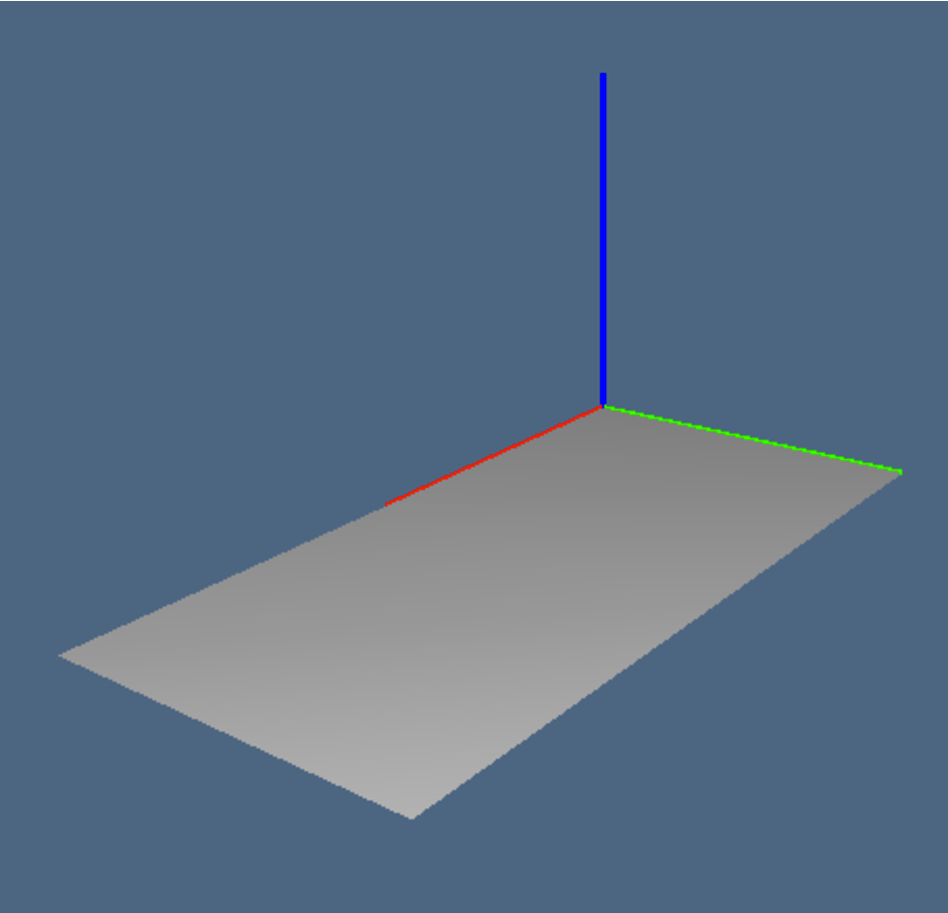
\includegraphics[height=0.25\linewidth,width=0.25\linewidth]{images/2D-non-manifold-a} 
   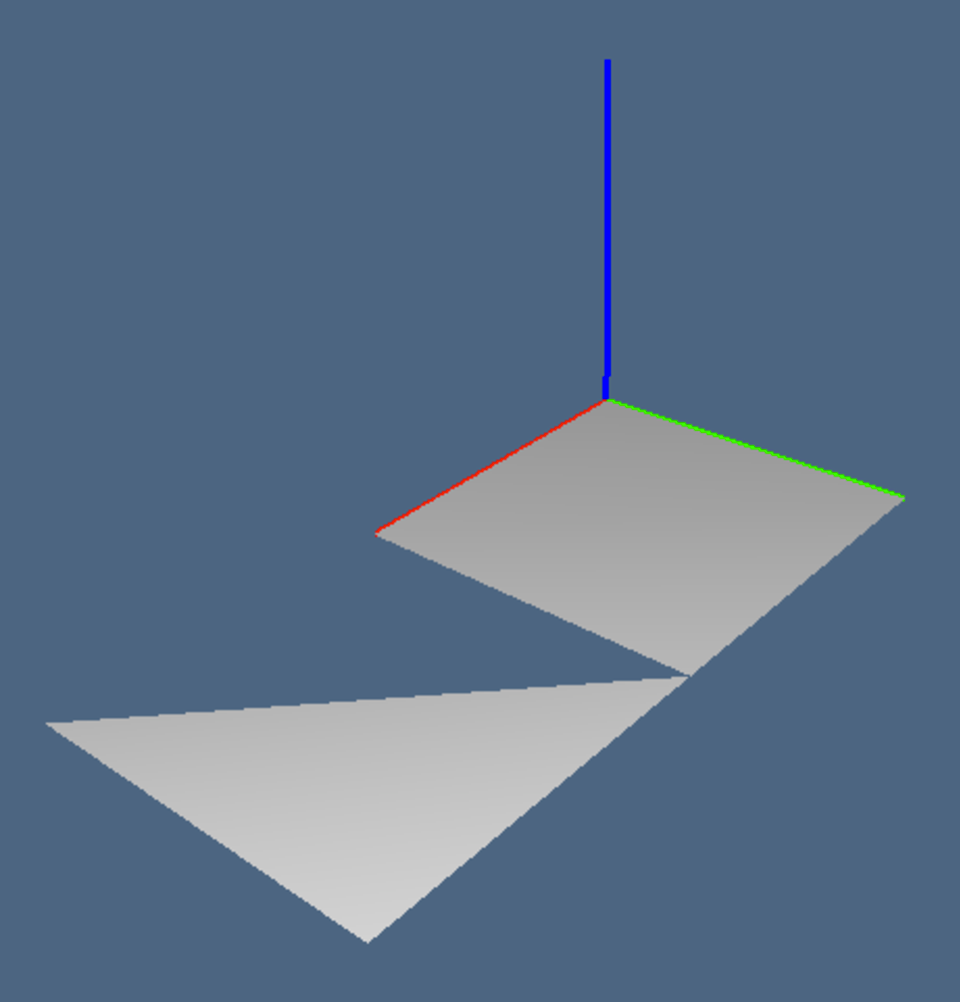
\includegraphics[height=0.25\linewidth,width=0.25\linewidth]{images/2D-non-manifold-b} 
   \caption{(a) Manifold two-dimensional space; (b) non-manifold space.}
   \label{fig:2D-non-manifold}
\end{figure}

\section{Matrix operations}

As we know, the LAR representation of topology is based on CSR representation of sparse binary (and integer) matrices.
Two Utility functions allow to query the number of rows and columns of a CSR matrix, independently from the low-level implementation (that in the following is provided by \emph{scipy.sparse}).
%-------------------------------------------------------------------------------
@d Query Matrix shape
@{def csrGetNumberOfRows(CSRmatrix):
    Int = CSRmatrix.shape[0]
    return Int
    
def csrGetNumberOfColumns(CSRmatrix):
    Int = CSRmatrix.shape[1]
    return Int
@}
%-------------------------------------------------------------------------------
%-------------------------------------------------------------------------------
@d Test examples of Query Matrix shape
@{print "\n>>> csrGetNumberOfRows"
print "\ncsrGetNumberOfRows(csrFV) =", csrGetNumberOfRows(csrFV)
print "\ncsrGetNumberOfRows(csrEV) =", csrGetNumberOfRows(csrEV)
print "\n>>> csrGetNumberOfColumns"
print "\ncsrGetNumberOfColumns(csrFV) =", csrGetNumberOfColumns(csrFV)
print "\ncsrGetNumberOfColumns(csrEV) =", csrGetNumberOfColumns(csrEV)
@}
%-------------------------------------------------------------------------------

\paragraph{}

%-------------------------------------------------------------------------------
@d Sparse to dense matrix transformation
@{def csr2DenseMatrix(CSRm):
    nrows = csrGetNumberOfRows(CSRm)
    ncolumns = csrGetNumberOfColumns(CSRm)
    ScipyMat = zeros((nrows,ncolumns),int)
    C = CSRm.tocoo()
    for triple in zip(C.row,C.col,C.data):
        ScipyMat[triple[0],triple[1]] = triple[2]
    return ScipyMat
@}
%-------------------------------------------------------------------------------
%-------------------------------------------------------------------------------
@d Test examples of Sparse to dense matrix transformation
@{print "\n>>> csr2DenseMatrix"
print "\nFV =\n", csr2DenseMatrix(csrFV)
print "\nEV =\n", csr2DenseMatrix(csrEV)
@}
%-------------------------------------------------------------------------------

\paragraph{Characteristic matrices}
Let us compute and show in dense form the characteristic matrices of 2- and 1-cells of the simple manifold just defined.
By running the file \texttt{test/py/larcc/ex8.py} the reader will get the two matrices shown in Example~\ref{ex:denseMat}
%-------------------------------------------------------------------------------
@o test/py/larcc/ex8.py
@{from larcc import *
@< Test example of Brc to Csr transformation @>
@< Test examples of Sparse to dense matrix transformation @>
@}
%-------------------------------------------------------------------------------
 
\begin{example}[Dense Characteristic matrices]\label{ex:denseMat}
Let us notice that the two matrices below have the some numbers of columns (indexed by vertices of the cell decomposition).
This very fact allows to multiply one matrix for the other transposed, and hence to compute the matrix form of linear operators between the spaces of cells of various dimensions.
\[
\texttt{FV} =
\begin{minipage}[c]{0.29\linewidth}
\begin{verbatim}
[[1 1 0 1 0 0]
 [0 1 1 0 1 0]
 [0 1 0 1 1 0]
 [0 0 1 0 1 1]]
\end{verbatim}
\end{minipage}
\qquad
\texttt{EV} =
\begin{minipage}[c]{0.29\linewidth}
\begin{verbatim}
[[1 1 0 0 0 0]
 [1 0 0 1 0 0]
 [0 1 1 0 0 0]
 [0 1 0 1 0 0]
 [0 1 0 0 1 0]
 [0 0 1 0 1 0]
 [0 0 1 0 0 1]
 [0 0 0 1 1 0]
 [0 0 0 0 1 1]]
\end{verbatim}
\end{minipage}
\]
\end{example}

\paragraph{Matrix product and transposition}

The following macro provides the IDE interface for the two main matrix operations required by LARCC, the binary product of compatible matrices and the unary transposition of matrices.

%-------------------------------------------------------------------------------
@d Matrix product and transposition
@{def matrixProduct(CSRm1,CSRm2):
    CSRm = CSRm1 * CSRm2
    return CSRm

def csrTranspose(CSRm):
    CSRm = CSRm.T
    return CSRm
@}
%-------------------------------------------------------------------------------

\begin{example}[Operators from edges to faces and vice-versa]\label{ex:denseMat}
As a general rule for operators between two spaces of chains of different dimensions supported by the \emph{same} cellular complex, we use names made by two characters, whose first letter correspond to the target space, and whose second letter to the domain space. Hence \texttt{FE} must be read as the operator from edges to faces. Of course, since this use correspond to see the first letter as the space generated by rows, and the second letter as the space generated by columns. Notice that the element $(i,j)$ of such matrices stores the number of vertices shared between the (row-)cell $i$ and the (column-)cell $j$.
\[
\texttt{FE} = \texttt{FV}\ \texttt{EV}^\top = 
\begin{minipage}[c]{0.29\linewidth}
\begin{verbatim}
[[2 2 1 2 1 0 0 1 0]
 [1 0 2 1 2 2 1 1 1]
 [1 1 1 2 2 1 0 2 1]
 [0 0 1 0 1 2 2 1 2]]
\end{verbatim}
\end{minipage}
\qquad
\texttt{EF} = \texttt{EV}\ \texttt{FV}^\top = 
\begin{minipage}[c]{0.29\linewidth}
\begin{verbatim}
[[2 1 1 0]
 [2 0 1 0]
 [1 2 1 1]
 [2 1 2 0]
 [1 2 2 1]
 [0 2 1 2]
 [0 1 0 2]
 [1 1 2 1]
 [0 1 1 2]]
\end{verbatim}
\end{minipage}
\]
\end{example}

\begin{figure}[htbp] %  figure placement: here, top, bottom, or page
   \centering
   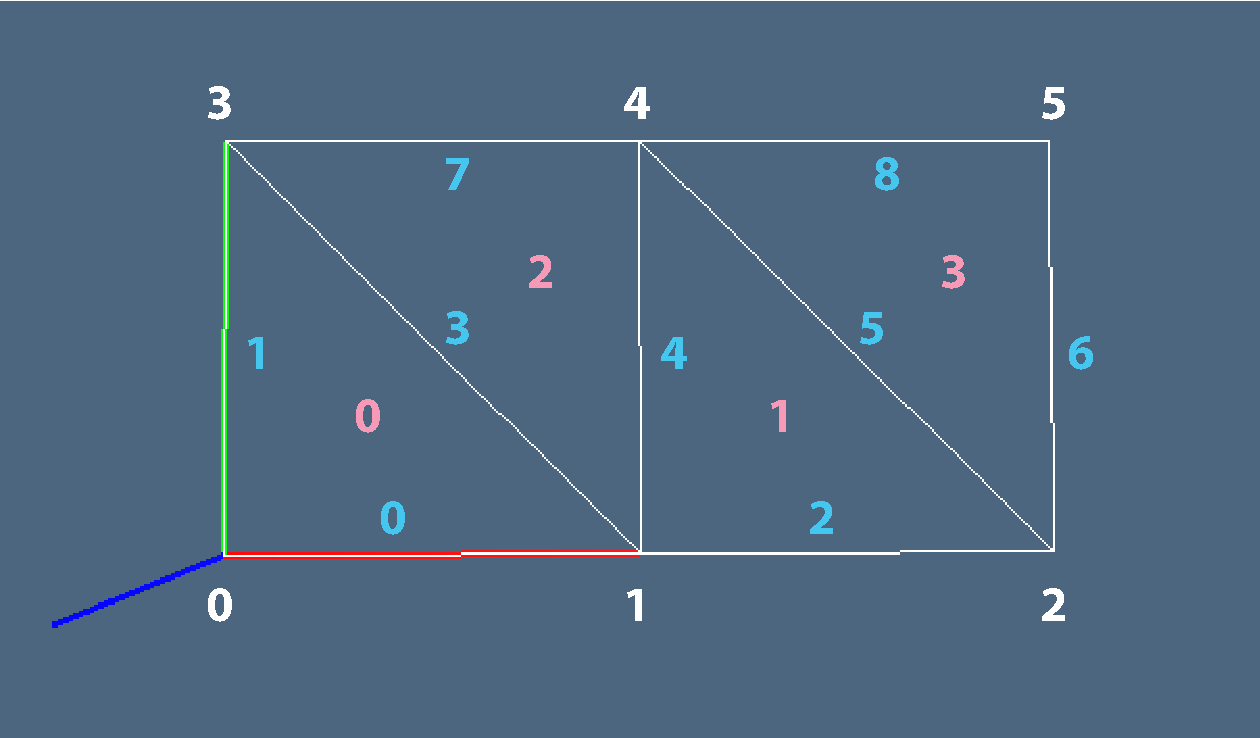
\includegraphics[width=0.6\linewidth]{images/2complex} 
   \caption{example caption}
   \label{fig:2complex}
\end{figure}
%-------------------------------------------------------------------------------
@d Matrix filtering to produce the boundary matrix
@{def csrBoundaryFilter(CSRm, facetLengths):
    maxs = [max(CSRm[k].data) for k in range(CSRm.shape[0])]
    inputShape = CSRm.shape
    coo = CSRm.tocoo()
    for k in range(len(coo.data)):
        if coo.data[k]==maxs[coo.row[k]]: coo.data[k] = 1
        else: coo.data[k] = 0
    mtx = coo_matrix((coo.data, (coo.row, coo.col)), shape=inputShape)
    out = mtx.tocsr()
    return out
@}
%-------------------------------------------------------------------------------
%-------------------------------------------------------------------------------
@d Test example of Matrix filtering to produce the boundary matrix
@{print "\n>>> csrBoundaryFilter"
csrEF = matrixProduct(csrFV, csrTranspose(csrEV)).T
facetLengths = [csrCell.getnnz() for csrCell in csrEV]
CSRm = csrBoundaryFilter(csrEF, facetLengths).T
print "\ncsrMaxFilter(csrFE) =\n", csr2DenseMatrix(CSRm)
@}
%-------------------------------------------------------------------------------
%-------------------------------------------------------------------------------
@d Matrix filtering via a generic predicate
@{def csrPredFilter(CSRm, pred):
	# can be done in parallel (by rows)
	coo = CSRm.tocoo()
	triples = [[row,col,val] for row,col,val 
				in zip(coo.row,coo.col,coo.data) if pred(val)]
	i, j, data = TRANS(triples)
	CSRm = scipy.sparse.coo_matrix((data,(i,j)),CSRm.shape).tocsr()
	return CSRm
@}
%-------------------------------------------------------------------------------
%-------------------------------------------------------------------------------
@d Test example of Matrix filtering via a generic predicate
@{print "\n>>> csrPredFilter"
CSRm = csrPredFilter(matrixProduct(csrFV, csrTranspose(csrEV)).T, GE(2)).T
print "\nccsrPredFilter(csrFE) =\n", csr2DenseMatrix(CSRm)
@}
%-------------------------------------------------------------------------------

\section{Topological operations}

\subsection{Incidence and adjacency operators}


\subsection{Boundary and coboundary operators}

%-------------------------------------------------------------------------------
@d From cells and facets to boundary operator
@{def boundary(cells,facets):
    csrCV = csrCreate(cells)
    csrFV = csrCreate(facets)
    csrFC = matrixProduct(csrFV, csrTranspose(csrCV))
    facetLengths = [csrCell.getnnz() for csrCell in csrCV]
    return csrBoundaryFilter(csrFC,facetLengths)

def coboundary(cells,facets):
    Boundary = boundary(cells,facets)
    return csrTranspose(Boundary)
@}
%-------------------------------------------------------------------------------
%-------------------------------------------------------------------------------
@d Test examples of From cells and facets to boundary operator
@{V = [[0.0, 0.0, 0.0], [1.0, 0.0, 0.0], [0.0, 1.0, 0.0], [1.0, 1.0, 0.0], 
[0.0, 0.0, 1.0], [1.0, 0.0, 1.0], [0.0, 1.0, 1.0], [1.0, 1.0, 1.0]]

CV =[[0, 1, 2, 4], [1, 2, 4, 5], [2, 4, 5, 6], [1, 2, 3, 5], [2, 3, 5, 6], 
[3, 5, 6, 7]]

FV =[[0, 1, 2], [0, 1, 4], [0, 2, 4], [1, 2, 3], [1, 2, 4], [1, 2, 5], 
[1, 3, 5], [1, 4, 5], [2, 3, 5], [2, 3, 6], [2, 4, 5], [2, 4, 6], [2, 5, 6], 
[3, 5, 6], [3, 5, 7], [3, 6, 7], [4, 5, 6], [5, 6, 7]]

EV =[[0, 1], [0, 2], [0, 4], [1, 2], [1, 3], [1, 4], [1, 5], [2, 3], [2, 4], 
[2, 5], [2, 6], [3, 5], [3, 6], [3, 7], [4, 5], [4, 6], [5, 6], [5, 7], 
[6, 7]]

print "\ncoboundary_2 =\n", csr2DenseMatrix(coboundary(CV,FV))
print "\ncoboundary_1 =\n", csr2DenseMatrix(coboundary(FV,EV))
print "\ncoboundary_0 =\n", csr2DenseMatrix(coboundary(EV,AA(LIST)(range(len(V)))))
@}
%-------------------------------------------------------------------------------
%-------------------------------------------------------------------------------
@d From cells and facets to boundary cells
@{def zeroChain(cells):
	pass

def totalChain(cells):
	return csrCreate([[0] for cell in cells])

def boundaryCells(cells,facets):
	csrBoundaryMat = boundary(cells,facets)
	csrChain = totalChain(cells)
	csrBoundaryChain = matrixProduct(csrBoundaryMat, csrChain)
	for k,value in enumerate(csrBoundaryChain.data):
		if value % 2 == 0: csrBoundaryChain.data[k] = 0
	boundaryCells = [k for k,val in enumerate(csrBoundaryChain.data.tolist()) if val == 1]
	return boundaryCells
@}
%-------------------------------------------------------------------------------
%-------------------------------------------------------------------------------
@d Test examples of From cells and facets to boundary cells
@{boundaryCells_2 = boundaryCells(CV,FV)
boundaryCells_1 = boundaryCells([FV[k] for k in boundaryCells_2],EV)

print "\nboundaryCells_2 =\n", boundaryCells_2
print "\nboundaryCells_1 =\n", boundaryCells_1

boundary = (V,[FV[k] for k in boundaryCells_2])
VIEW(EXPLODE(1.5,1.5,1.5)(MKPOLS(boundary)))
@}
%-------------------------------------------------------------------------------
%-------------------------------------------------------------------------------
@d Signed boundary matrix for simplicial models
@{def signedBoundary (V,CV,FV):
	# compute the set of pairs of indices to [boundary face,incident coface]
	coo = boundary(CV,FV).tocoo()
	pairs = [[coo.row[k],coo.col[k]] for k,val in enumerate(coo.data) if val != 0]
	
	# compute the [face, coface] pair as vertex lists
	vertLists = [[FV[pair[0]], CV[pair[1]]]for pair in pairs]
	
	# compute two n-cells to compare for sign
	cellPairs = [ [list(set(coface).difference(face))+face,coface] 
					for face,coface in vertLists]
	
	# compute the local indices of missing boundary cofaces
	missingVertIndices = [ coface.index(list(set(coface).difference(face))[0]) 
							for face,coface in vertLists]
	
	# compute the point matrices to compare for sign
	pointArrays = [ [[V[k]+[1.0] for k in facetCell], [V[k]+[1.0] for k in cofaceCell]] 
					for facetCell,cofaceCell in cellPairs]
	
	# signed incidence coefficients
	cofaceMats = TRANS(pointArrays)[1]
	cofaceSigns = AA(SIGN)(AA(np.linalg.det)(cofaceMats))
	faceSigns = AA(C(POWER)(-1))(missingVertIndices)
	signPairProd = AA(PROD)(TRANS([cofaceSigns,faceSigns]))
	
	# signed boundary matrix
	csrSignedBoundaryMat = csr_matrix( (signPairProd,TRANS(pairs)) )
	return csrSignedBoundaryMat
@}
%-------------------------------------------------------------------------------
%-------------------------------------------------------------------------------
@d Oriented boundary cells for simplicial models
@{def signedBoundaryCells(verts,cells,facets):
	csrBoundaryMat = signedBoundary(verts,cells,facets)
	csrTotalChain = totalChain(cells)
	csrBoundaryChain = matrixProduct(csrBoundaryMat, csrTotalChain)
	coo = csrBoundaryChain.tocoo()
	boundaryCells = list(coo.row * coo.data)
	return AA(int)(boundaryCells)
@}
%-------------------------------------------------------------------------------
\paragraph{Orienting polytopal cells}
\begin{description}
	\item[input]:  "cell" indices of a convex and solid polytopes and "V" vertices;
	\item[output]:  biggest "simplex" indices spanning the polytope.
	\item[\tt m]: number of cell vertices
	\item[\tt d]: dimension (number of coordinates) of cell vertices
	\item[\tt d+1]: number of simplex vertices
	\item[\tt vcell]: cell vertices
	\item[\tt vsimplex]: simplex vertices
	\item[\tt Id]: identity matrix
	\item[\tt basis]: orthonormal spanning set of vectors $e_k$
	\item[\tt vector]: position vector of a simplex vertex in translated coordinates
	\item[\tt unUsedIndices]: cell indices not moved to simplex
\end{description}

%-------------------------------------------------------------------------------
@d Oriented boundary cells for simplicial models
@{def pivotSimplices(V,CV,d=3):
	simplices = []
	for cell in CV:
		vcell = np.array([V[v] for v in cell])
		m, simplex = len(cell), []
		# translate the cell: for each k, vcell[k] -= vcell[0], and simplex[0] := cell[0]
		for k in range(m-1,-1,-1): vcell[k] -= vcell[0]
		# simplex = [0], basis = [], tensor = Id(d+1)
		simplex += [cell[0]]
		basis = []
		tensor = np.array(IDNT(d))
		# look for most far cell vertex
		dists = [SUM([SQR(x) for x in v])**0.5 for v in vcell]
		maxDistIndex = max(enumerate(dists),key=lambda x: x[1])[0]
		vector = np.array([vcell[maxDistIndex]])
		# normalize vector
		den=(vector**2).sum(axis=-1) **0.5
		basis = [vector/den]
		simplex += [cell[maxDistIndex]]
		unUsedIndices = [h for h in cell if h not in simplex]
		
		# for k in {2,d+1}:
		for k in range(2,d+1):
			# update the orthonormal tensor
			e = basis[-1]
			tensor = tensor - np.dot(e.T, e)
			# compute the index h of a best vector
			# look for most far cell vertex
			dists = [SUM([SQR(x) for x in np.dot(tensor,v)])**0.5
			if h in unUsedIndices else 0.0
			for (h,v) in zip(cell,vcell)]
			# insert the best vector index h in output simplex
			maxDistIndex = max(enumerate(dists),key=lambda x: x[1])[0]
			vector = np.array([vcell[maxDistIndex]])
			# normalize vector
			den=(vector**2).sum(axis=-1) **0.5
			basis += [vector/den]
			simplex += [cell[maxDistIndex]]
			unUsedIndices = [h for h in cell if h not in simplex]
		simplices += [simplex]
	return simplices

def simplexOrientations(V,simplices):
	vcells = [[V[v]+[1.0] for v in simplex] for simplex in simplices]
	return [SIGN(np.linalg.det(vcell)) for vcell in vcells]
@}
%-------------------------------------------------------------------------------
%-------------------------------------------------------------------------------
@d Computation of cell adjacencies
@{def larCellAdjacencies(CSRm):
    CSRm = matrixProduct(CSRm,csrTranspose(CSRm))
    return CSRm
@}
%-------------------------------------------------------------------------------
%-------------------------------------------------------------------------------
@d Test examples of Computation of cell adjacencies
@{print "\n>>> larCellAdjacencies"
adj_2_cells = larCellAdjacencies(csrFV)
print "\nadj_2_cells =\n", csr2DenseMatrix(adj_2_cells)
adj_1_cells = larCellAdjacencies(csrEV)
print "\nadj_1_cells =\n", csr2DenseMatrix(adj_1_cells)
@}
%-------------------------------------------------------------------------------
%-------------------------------------------------------------------------------
@d Extraction of facets of a cell complex
@{def setup(model,dim):
    V, cells = model
    csr = csrCreate(cells)
    csrAdjSquareMat = larCellAdjacencies(csr)
    csrAdjSquareMat = csrPredFilter(csrAdjSquareMat, GE(dim)) # ? HOWTODO ?
    return V,cells,csr,csrAdjSquareMat

def larFacets(model,dim=3):
    """
        Estraction of (d-1)-cellFacets from "model" := (V,d-cells)
        Return (V, (d-1)-cellFacets)
		"""
    V,cells,csr,csrAdjSquareMat = setup(model,dim)
    cellFacets = []
    # for each input cell i
    for i in range(len(cells)):
        adjCells = csrAdjSquareMat[i].tocoo()
        cell1 = csr[i].tocoo().col
        pairs = zip(adjCells.col,adjCells.data)
        for j,v in pairs:
            if (i<j):
                cell2 = csr[j].tocoo().col
                cell = list(set(cell1).intersection(cell2))
                cellFacets.append(sorted(cell))
    # sort and remove duplicates
    cellFacets = sorted(AA(list)(set(AA(tuple)(cellFacets))))
    return V,cellFacets
@}
%-------------------------------------------------------------------------------
%-------------------------------------------------------------------------------
@d Test examples of Extraction of facets of a cell complex
@{V = [[0.,0.],[3.,0.],[0.,3.],[3.,3.],[1.,2.],[2.,2.],[1.,1.],[2.,1.]]
FV = [[0,1,6,7],[0,2,4,6],[4,5,6,7],[1,3,5,7],[2,3,4,5],[0,1,2,3]]

_,EV = larFacets((V,FV),dim=2)
print "\nEV =",EV
VIEW(EXPLODE(1.5,1.5,1.5)(MKPOLS((V,EV))))

FV = [[0,1,3],[1,2,4],[2,4,5],[3,4,6],[4,6,7],[5,7,8], # full
	[1,3,4],[4,5,7], # empty
	[0,1,2],[6,7,8],[0,3,6],[2,5,8]] # exterior
		
_,EV = larFacets((V,FV),dim=2)
print "\nEV =",EV
@}
%-------------------------------------------------------------------------------

\section{Exporting the library}

\subsection{MIT licence}
%-------------------------------------------------------------------------------
@d The MIT Licence
@{
"""
The MIT License
===============
    
Permission is hereby granted, free of charge, to any person obtaining
a copy of this software and associated documentation files (the
'Software'), to deal in the Software without restriction, including
without limitation the rights to use, copy, modify, merge, publish,
distribute, sublicense, and/or sell copies of the Software, and to
permit persons to whom the Software is furnished to do so, subject to
the following conditions:

The above copyright notice and this permission notice shall be
included in all copies or substantial portions of the Software.

THE SOFTWARE IS PROVIDED 'AS IS', WITHOUT WARRANTY OF ANY KIND,
EXPRESS OR IMPLIED, INCLUDING BUT NOT LIMITED TO THE WARRANTIES OF
MERCHANTABILITY, FITNESS FOR A PARTICULAR PURPOSE AND NONINFRINGEMENT.
IN NO EVENT SHALL THE AUTHORS OR COPYRIGHT HOLDERS BE LIABLE FOR ANY
CLAIM, DAMAGES OR OTHER LIABILITY, WHETHER IN AN ACTION OF CONTRACT,
TORT OR OTHERWISE, ARISING FROM, OUT OF OR IN CONNECTION WITH THE
SOFTWARE OR THE USE OR OTHER DEALINGS IN THE SOFTWARE.
"""
@}
%-------------------------------------------------------------------------------
\subsection{Importing of modules or packages}
%-------------------------------------------------------------------------------
@d Importing of modules or packages
@{from pyplasm import *
import collections
import scipy
import numpy as np
from scipy import zeros,arange,mat,amin,amax
from scipy.sparse import vstack,hstack,csr_matrix,coo_matrix,lil_matrix,triu

from lar2psm import *
@}
%-------------------------------------------------------------------------------

\subsection{Writing the library file}

%-------------------------------------------------------------------------------
@o lib/py/larcc.py
@{# -*- coding: utf-8 -*-
""" Basic LARCC library """
@< The MIT Licence @>
@< Importing of modules or packages @>
@< From list of triples to scipy.sparse @>
@< Brc to Coo transformation @>
@< Coo to Csr transformation @>
@< Brc to Csr transformation @>
@< Query Matrix shape @>
@< Sparse to dense matrix transformation @>
@< Matrix product and transposition @>
@< Matrix filtering to produce the boundary matrix @>
@< Matrix filtering via a generic predicate @>
@< From cells and facets to boundary operator @>
@< From cells and facets to boundary cells @>
@< Signed boundary matrix for simplicial models @>
@< Oriented boundary cells for simplicial models @>
@< Computation of cell adjacencies @>
@< Extraction of facets of a cell complex @>

if __name__ == "__main__": 
	@< Test examples @>
@}
%-------------------------------------------------------------------------------

\section{Unit tests}


%-------------------------------------------------------------------------------
@d Test examples
@{
@< Test example of Brc to Coo transformation @>
@< Test example of Coo to Csr transformation @>
@< Test example of Brc to Csr transformation @>
@< Test examples of Query Matrix shape @>
@< Test examples of Sparse to dense matrix transformation @>
@< Test example of Matrix filtering to produce the boundary matrix @>
@< Test example of Matrix filtering via a generic predicate @>
@< Test examples of From cells and facets to boundary operator @>
@< Test examples of From cells and facets to boundary cells @>
@< Test examples of Computation of cell adjacencies @>
@< Test examples of Extraction of facets of a cell complex @>
@}
%-------------------------------------------------------------------------------


\appendix

\section{Appendix: Tutorials}


\subsection{Model generation, skeleton and boundary extraction}

%-------------------------------------------------------------------------------
@o test/py/larcc/ex1.py
@{
from larcc import *
from largrid import *
@< input of 2D topology and geometry data @>
@< characteristic matrices @>
@< incidence matrix @>
@< boundary and coboundary operators @>
@< product of cell complexes @>
@< 2-skeleton extraction @>
@< 1-skeleton extraction  @>
@< 0-coboundary computation @>
@< 1-coboundary computation @>
@< 2-coboundary computation @>
@< boundary chain visualisation @>
@}
%-------------------------------------------------------------------------------

%-------------------------------------------------------------------------------
@d input of 2D topology and geometry data
@{
# input of geometry and topology  
V2 = [[4,10],[8,10],[14,10],[8,7],[14,7],[4,4],[8,4],[14,4]]
EV = [[0,1],[1,2],[3,4],[5,6],[6,7],[0,5],[1,3],[2,4],[3,6],[4,7]]
FV = [[0,1,3,5,6],[1,2,3,4],[3,4,6,7]]
@}
%-------------------------------------------------------------------------------

%-------------------------------------------------------------------------------
@d characteristic matrices
@{# characteristic matrices
csrFV = csrCreate(FV)
csrEV = csrCreate(EV)
print "\nFV =\n", csr2DenseMatrix(csrFV)
print "\nEV =\n", csr2DenseMatrix(csrEV)
@}
%-------------------------------------------------------------------------------

%-------------------------------------------------------------------------------
@d incidence matrix
@{# product
csrEF = matrixProduct(csrEV, csrTranspose(csrFV))
print "\nEF =\n", csr2DenseMatrix(csrEF)
@}
%-------------------------------------------------------------------------------

%-------------------------------------------------------------------------------
@d boundary and coboundary operators
@{# boundary and coboundary operators
facetLengths = [csrCell.getnnz() for csrCell in csrEV]
boundary = csrBoundaryFilter(csrEF,facetLengths)
coboundary_1 = csrTranspose(boundary)
print "\ncoboundary_1 =\n", csr2DenseMatrix(coboundary_1)
@}
%-------------------------------------------------------------------------------

%-------------------------------------------------------------------------------
@d product of cell complexes
@{# product operator
mod_2D = (V2,FV)
V1,topol_0 = [[0.],[1.],[2.]], [[0],[1],[2]]
topol_1 = [[0,1],[1,2]]
mod_0D = (V1,topol_0)
mod_1D = (V1,topol_1)
V3,CV = larModelProduct([mod_2D,mod_1D])
mod_3D = (V3,CV)
VIEW(EXPLODE(1.2,1.2,1.2)(MKPOLS(mod_3D)))
print "\nk_3 =", len(CV), "\n"
@}
%-------------------------------------------------------------------------------

%-------------------------------------------------------------------------------
@d 2-skeleton extraction
@{# 2-skeleton of the 3D product complex
mod_2D_1 = (V2,EV)
mod_3D_h2 = larModelProduct([mod_2D,mod_0D])
mod_3D_v2 = larModelProduct([mod_2D_1,mod_1D])
_,FV_h = mod_3D_h2
_,FV_v = mod_3D_v2
FV3 = FV_h + FV_v
SK2 = (V3,FV3)
VIEW(EXPLODE(1.2,1.2,1.2)(MKPOLS(SK2)))
print "\nk_2 =", len(FV3), "\n"
@}
%-------------------------------------------------------------------------------

%-------------------------------------------------------------------------------
@d 1-skeleton extraction 
@{# 1-skeleton of the 3D product complex 
mod_2D_0 = (V2,AA(LIST)(range(len(V2))))
mod_3D_h1 = larModelProduct([mod_2D_1,mod_0D])
mod_3D_v1 = larModelProduct([mod_2D_0,mod_1D])
_,EV_h = mod_3D_h1
_,EV_v = mod_3D_v1
EV3 = EV_h + EV_v
SK1 = (V3,EV3)
VIEW(EXPLODE(1.2,1.2,1.2)(MKPOLS(SK1)))
print "\nk_1 =", len(EV3), "\n"
@}
%-------------------------------------------------------------------------------

%-------------------------------------------------------------------------------
@d 0-coboundary computation
@{# boundary and coboundary operators
np.set_printoptions(threshold=sys.maxint)
csrFV3 = csrCreate(FV3)
csrEV3 = csrCreate(EV3)
csrVE3 = csrTranspose(csrEV3)
facetLengths = [csrCell.getnnz() for csrCell in csrEV3]
boundary = csrBoundaryFilter(csrVE3,facetLengths)
coboundary_0 = csrTranspose(boundary)
print "\ncoboundary_0 =\n", csr2DenseMatrix(coboundary_0)
@}
%-------------------------------------------------------------------------------

%-------------------------------------------------------------------------------
@d 1-coboundary computation
@{csrEF3 = matrixProduct(csrEV3, csrTranspose(csrFV3))
facetLengths = [csrCell.getnnz() for csrCell in csrFV3]
boundary = csrBoundaryFilter(csrEF3,facetLengths)
coboundary_1 = csrTranspose(boundary)
print "\ncoboundary_1.T =\n", csr2DenseMatrix(coboundary_1.T)
@}
%-------------------------------------------------------------------------------

%-------------------------------------------------------------------------------
@d 2-coboundary computation
@{csrCV = csrCreate(CV)
csrFC3 = matrixProduct(csrFV3, csrTranspose(csrCV))
facetLengths = [csrCell.getnnz() for csrCell in csrCV]
boundary = csrBoundaryFilter(csrFC3,facetLengths)
coboundary_2 = csrTranspose(boundary)
print "\ncoboundary_2 =\n", csr2DenseMatrix(coboundary_2)
@}
%-------------------------------------------------------------------------------

%-------------------------------------------------------------------------------
@d boundary chain visualisation
@{# boundary chain visualisation
boundaryCells_2 = boundaryCells(CV,FV3)
boundary = (V3,[FV3[k] for k in boundaryCells_2])
VIEW(EXPLODE(1.5,1.5,1.5)(MKPOLS(boundary)))
@}
%-------------------------------------------------------------------------------



\subsection{Boundary of 3D simplicial grid}

%-------------------------------------------------------------------------------
@o test/py/larcc/ex2.py
@{
@< boundary of 3D simplicial grid @>
@}
%-------------------------------------------------------------------------------

%-------------------------------------------------------------------------------
@d boundary of 3D simplicial grid
@{from simplexn import *
from larcc import *

V,CV = larSimplexGrid([10,10,3])
VIEW(EXPLODE(1.5,1.5,1.5)(MKPOLS((V,CV))))
SK2 = (V,larSimplexFacets(CV))
VIEW(EXPLODE(1.5,1.5,1.5)(MKPOLS(SK2)))
_,FV = SK2
SK1 = (V,larSimplexFacets(FV))
_,EV = SK1
VIEW(EXPLODE(1.5,1.5,1.5)(MKPOLS(SK1)))

boundaryCells_2 = boundaryCells(CV,FV)
boundary = (V,[FV[k] for k in boundaryCells_2])
VIEW(EXPLODE(1.5,1.5,1.5)(MKPOLS(boundary)))
print "\nboundaryCells_2 =\n", boundaryCells_2
@}
%-------------------------------------------------------------------------------


\subsection{Oriented boundary of a random simplicial complex}


%-------------------------------------------------------------------------------
@o test/py/larcc/ex3.py
@{@< Importing external modules @>
@< Generating and viewing a random 3D simplicial complex @>
@< Computing and viewing its non-oriented boundary @>
@< Computing and viewing its oriented boundary @>
@}
%-------------------------------------------------------------------------------


%-------------------------------------------------------------------------------
@d Importing external modules
@{from simplexn import *
from larcc import *
from scipy.spatial import Delaunay
import numpy as np
@}
%-------------------------------------------------------------------------------

%-------------------------------------------------------------------------------
@d Generating and viewing a random 3D simplicial complex
@{verts = np.random.rand(10000, 3) # 1000 points in 3-d
verts = [AA(lambda x: 2*x)(VECTDIFF([vert,[0.5,0.5,0.5]])) for vert in verts]
verts = [vert for vert in verts if VECTNORM(vert) < 1.0]
tetra = Delaunay(verts)
cells = [cell for cell in tetra.vertices.tolist()
         if  ((verts[cell[0]][2]<0) and (verts[cell[1]][2]<0) 
         		and (verts[cell[2]][2]<0) and (verts[cell[3]][2]<0) ) ]
V, CV = verts, cells
VIEW(MKPOL([V,AA(AA(lambda k:k+1))(CV),[]]))
@}
%-------------------------------------------------------------------------------

%-------------------------------------------------------------------------------
@d Computing and viewing its non-oriented boundary 
@{FV = larSimplexFacets(CV)
VIEW(MKPOL([V,AA(AA(lambda k:k+1))(FV),[]]))
boundaryCells_2 = boundaryCells(CV,FV)
print "\nboundaryCells_2 =\n", boundaryCells_2
bndry = (V,[FV[k] for k in boundaryCells_2])
VIEW(EXPLODE(1.5,1.5,1.5)(MKPOLS(bndry)))
@}
%-------------------------------------------------------------------------------

%-------------------------------------------------------------------------------
@d Computing and viewing its oriented boundary
@{boundaryCells_2 = signedBoundaryCells(V,CV,FV)
print "\nboundaryCells_2 =\n", boundaryCells_2
def swap(mylist): return [mylist[1]]+[mylist[0]]+mylist[2:]
boundaryFV = [FV[-k] if k<0 else swap(FV[k]) for k in boundaryCells_2]
bndry = (V,boundaryFV)
VIEW(EXPLODE(1.5,1.5,1.5)(MKPOLS(bndry)))
@}
%-------------------------------------------------------------------------------

\subsection{Oriented boundary of a simplicial grid}

%-------------------------------------------------------------------------------
@o test/py/larcc/ex4.py
@{@< Generate and view a 3D simplicial grid @>
@< Computing and viewing the 2-skeleton of simplicial grid @>
@< Computing and viewing the oriented boundary of simplicial grid @>
@}
%-------------------------------------------------------------------------------


%-------------------------------------------------------------------------------
@d Generate and view a 3D simplicial grid
@{from simplexn import *
from larcc import *
V,CV = larSimplexGrid([4,4,4])
VIEW(EXPLODE(1.5,1.5,1.5)(MKPOLS((V,CV))))
@}
%-------------------------------------------------------------------------------

%-------------------------------------------------------------------------------
@d Computing and viewing the 2-skeleton of simplicial grid
@{FV = larSimplexFacets(CV)
EV = larSimplexFacets(FV)
VIEW(EXPLODE(1.5,1.5,1.5)(MKPOLS((V,FV))))
@}
%-------------------------------------------------------------------------------

%-------------------------------------------------------------------------------
@d Computing and viewing the oriented boundary of simplicial grid
@{csrSignedBoundaryMat = signedBoundary (V,CV,FV)
boundaryCells_2 = signedBoundaryCells(V,CV,FV)
def swap(l): return [l[1],l[0],l[2]]
boundaryFV = [FV[-k] if k<0 else swap(FV[k]) for k in boundaryCells_2]
boundary = (V,boundaryFV)
VIEW(EXPLODE(1.5,1.5,1.5)(MKPOLS(boundary)))
@}
%-------------------------------------------------------------------------------


\subsection{Skeletons and oriented boundary of a simplicial complex}


%-------------------------------------------------------------------------------
@o test/py/larcc/ex5.py
@{@< Skeletons computation and vilualisation @>
@< Oriented boundary matrix visualization @>
@< Computation of oriented boundary cells @>
@}
%-------------------------------------------------------------------------------


%-------------------------------------------------------------------------------
@d Skeletons computation and vilualisation
@{from simplexn import *
from larcc import *
V,FV = larSimplexGrid([3,3])
VIEW(EXPLODE(1.5,1.5,1.5)(MKPOLS((V,FV))))
EV = larSimplexFacets(FV)
VIEW(EXPLODE(1.5,1.5,1.5)(MKPOLS((V,EV))))
VV = larSimplexFacets(EV)
VIEW(EXPLODE(1.5,1.5,1.5)(MKPOLS((V,VV))))
@}
%-------------------------------------------------------------------------------

%-------------------------------------------------------------------------------
@d Oriented boundary matrix visualization
@{np.set_printoptions(threshold='nan')
csrSignedBoundaryMat = signedBoundary (V,FV,EV)
Z = csr2DenseMatrix(csrSignedBoundaryMat)
print "\ncsrSignedBoundaryMat =\n", Z
from pylab import *
matshow(Z)
show()
@}
%-------------------------------------------------------------------------------

%-------------------------------------------------------------------------------
@d Computation of oriented boundary cells 
@{boundaryCells_1 = signedBoundaryCells(V,FV,EV)
print "\nboundaryCells_1 =\n", boundaryCells_1
def swap(mylist): return [mylist[1]]+[mylist[0]]+mylist[2:]
boundaryEV = [EV[-k] if k<0 else swap(EV[k]) for k in boundaryCells_1]
bndry = (V,boundaryEV)
VIEW(EXPLODE(1.5,1.5,1.5)(MKPOLS(bndry)))
@}
%-------------------------------------------------------------------------------

\subsection{Boundary of random 2D simplicial complex}

%-------------------------------------------------------------------------------
@o test/py/larcc/ex6.py
@{from simplexn import *
from larcc import *
from scipy.spatial import Delaunay
@< Test for quasi-equilateral triangles @>
@< Generation and selection of random triangles @>
@< Boundary computation and visualisation @>
@}
%-------------------------------------------------------------------------------


\begin{figure}[htbp] %  figure placement: here, top, bottom, or page
   \centering
   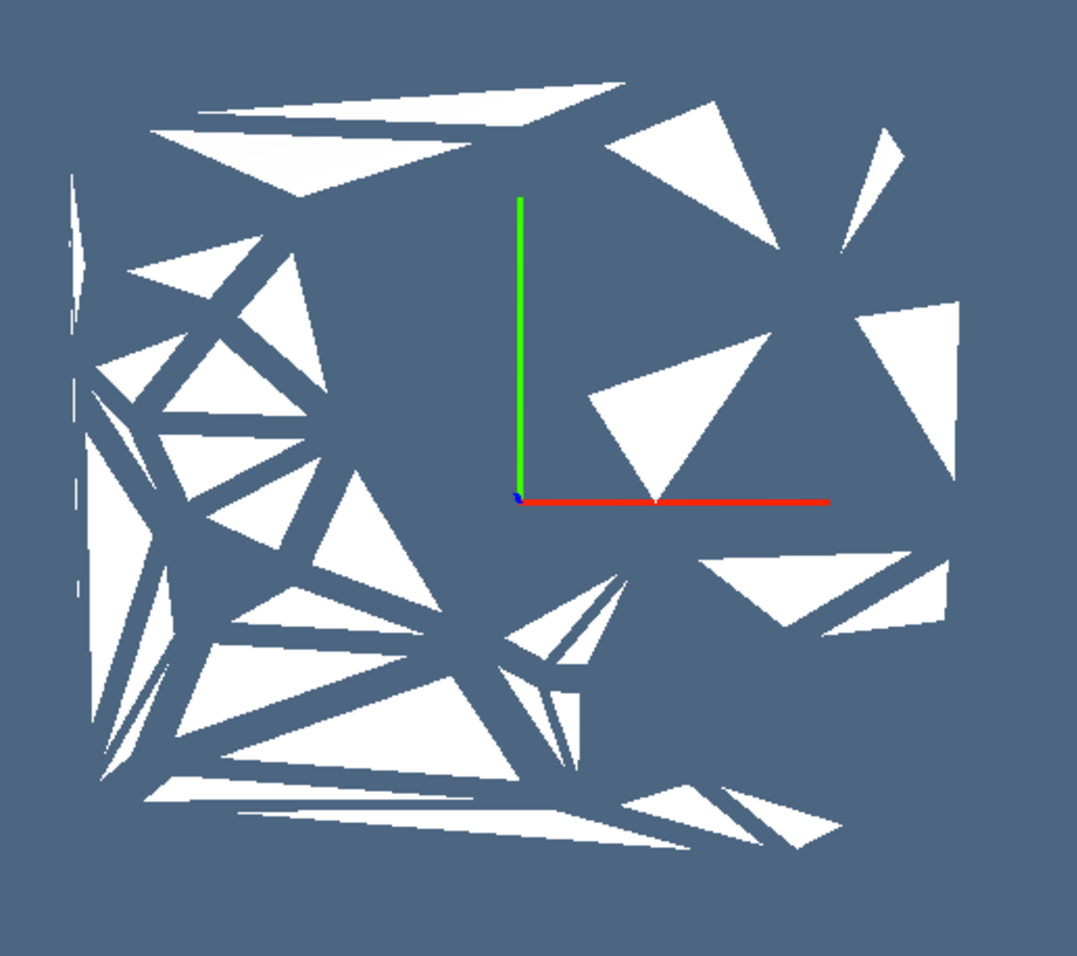
\includegraphics[height=0.25\linewidth,width=0.32\linewidth]{images/tria0} 
   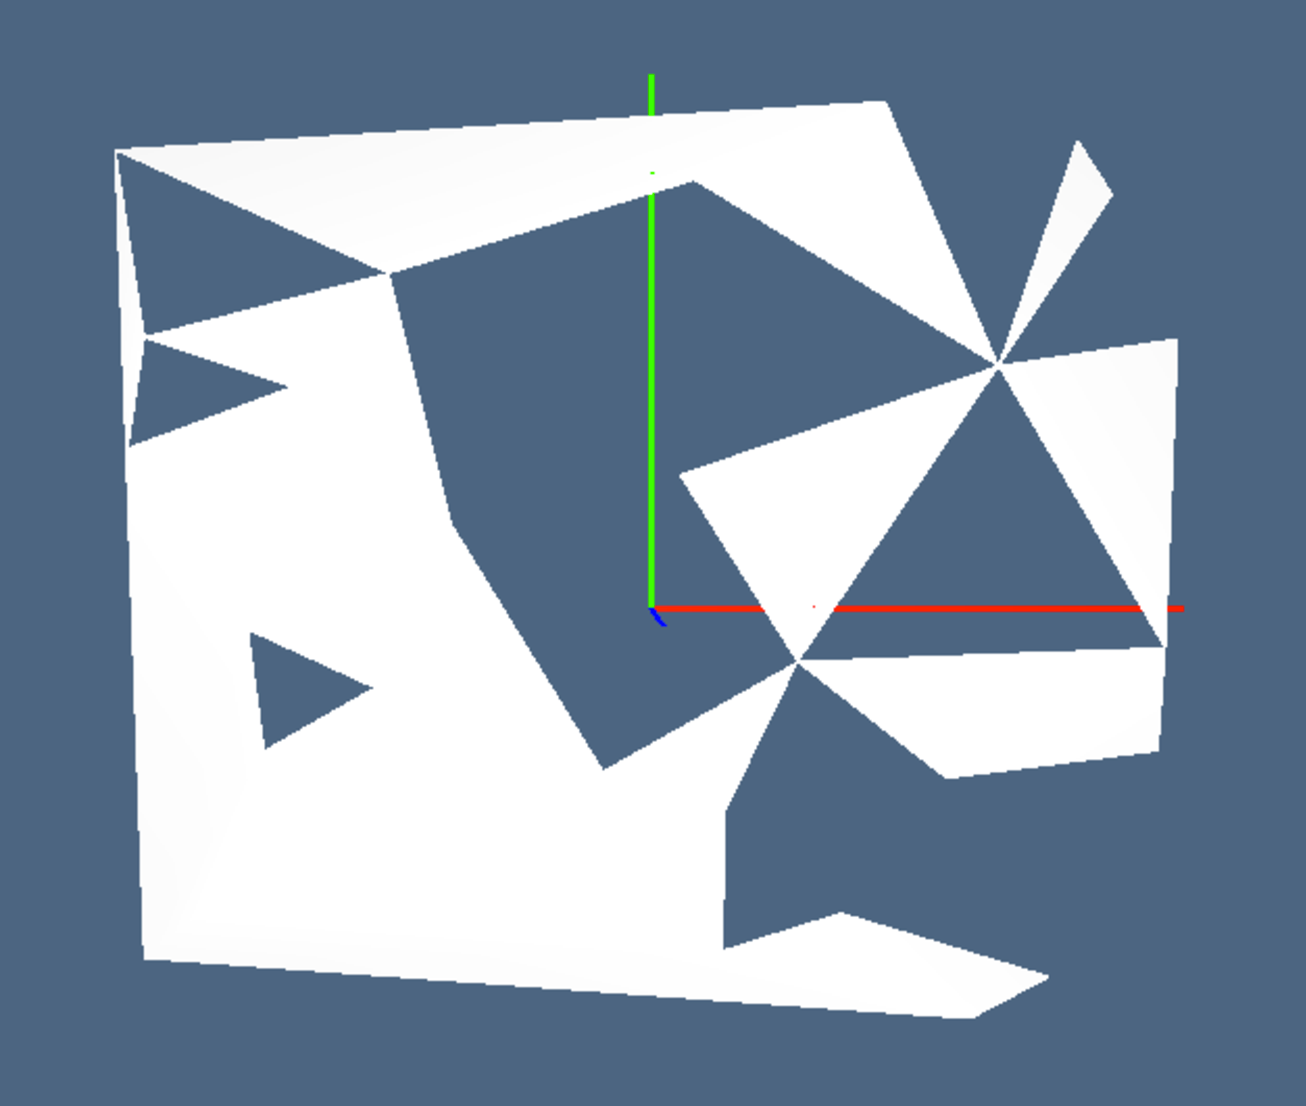
\includegraphics[height=0.25\linewidth,width=0.32\linewidth]{images/tria1} 
   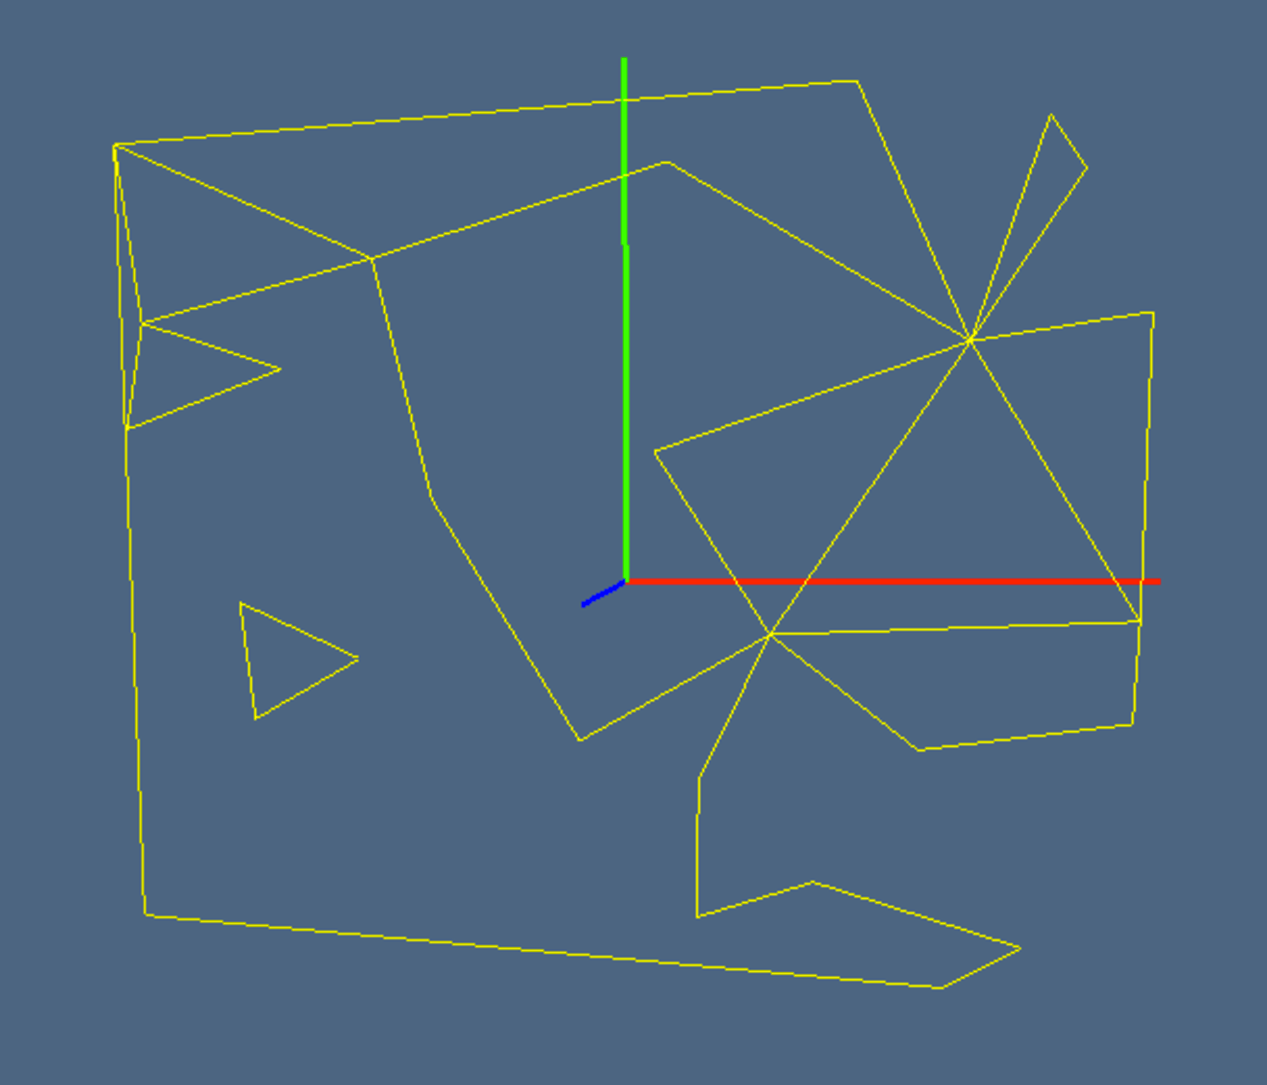
\includegraphics[height=0.25\linewidth,width=0.32\linewidth]{images/tria2} 
   \caption{example caption}
   \label{fig:example}
\end{figure}

%-------------------------------------------------------------------------------
@d Test for quasi-equilateral triangles
@{def quasiEquilateral(tria):
    a = VECTNORM(VECTDIFF(tria[0:2]))
    b = VECTNORM(VECTDIFF(tria[1:3]))
    c = VECTNORM(VECTDIFF([tria[0],tria[2]]))
    m = max(a,b,c)
    if m/a < 1.7 and m/b < 1.7 and m/c < 1.7: return True
    else: return False
@}
%-------------------------------------------------------------------------------

%-------------------------------------------------------------------------------
@d Generation and selection of random triangles 
@{verts = np.random.rand(20,2)
verts = (verts - [0.5,0.5]) * 2
triangles = Delaunay(verts)
cells = [ cell for cell in triangles.vertices.tolist()
         if (not quasiEquilateral([verts[k] for k in cell])) ]
V, FV = AA(list)(verts), cells
EV = larSimplexFacets(FV)
pols2D = MKPOLS((V,FV))
VIEW(EXPLODE(1.5,1.5,1.5)(pols2D))
@}
%-------------------------------------------------------------------------------

%-------------------------------------------------------------------------------
@d Boundary computation and visualisation 
@{boundaryCells_1 = signedBoundaryCells(V,FV,EV)
print "\nboundaryCells_1 =\n", boundaryCells_1
def swap(mylist): return [mylist[1]]+[mylist[0]]+mylist[2:]
boundaryEV = [EV[-k] if k<0 else swap(EV[k]) for k in boundaryCells_1]
bndry = (V,boundaryEV)
VIEW(STRUCT(MKPOLS(bndry) + pols2D))
VIEW(COLOR(RED)(STRUCT(MKPOLS(bndry))))
@}
%-------------------------------------------------------------------------------

%-------------------------------------------------------------------------------
@d Compute the topologically ordered chain of boundary vertices
@{
@}
%-------------------------------------------------------------------------------

%-------------------------------------------------------------------------------
@d Decompose a permutation into cycles 
@{def permutationOrbits(List):
	d = dict((i,int(x)) for i,x in enumerate(List))
	out = []
	while d:
		x = list(d)[0]
		orbit = []
		while x in d:
			orbit += [x],
			x = d.pop(x)
		out += [CAT(orbit)+orbit[0]]
	return out
		
if __name__ == "__main__":
	print [2, 3, 4, 5, 6, 7, 0, 1]
	print permutationOrbits([2, 3, 4, 5, 6, 7, 0, 1])
	print [3,9,8,4,10,7,2,11,6,0,1,5]
	print permutationOrbits([3,9,8,4,10,7,2,11,6,0,1,5])
@}
%-------------------------------------------------------------------------------

\subsection{Assemblies of simplices and hypercubes}

%-------------------------------------------------------------------------------
@o test/py/larcc/ex7.py
@{from simplexn import *
from larcc import *
from largrid import *
@< Definition of 1-dimensional LAR models @>
@< Assembly generation of squares and triangles @>
@< Assembly generation  of cubes and tetrahedra @>
@}
%-------------------------------------------------------------------------------

\begin{figure}[htbp] %  figure placement: here, top, bottom, or page
   \centering
   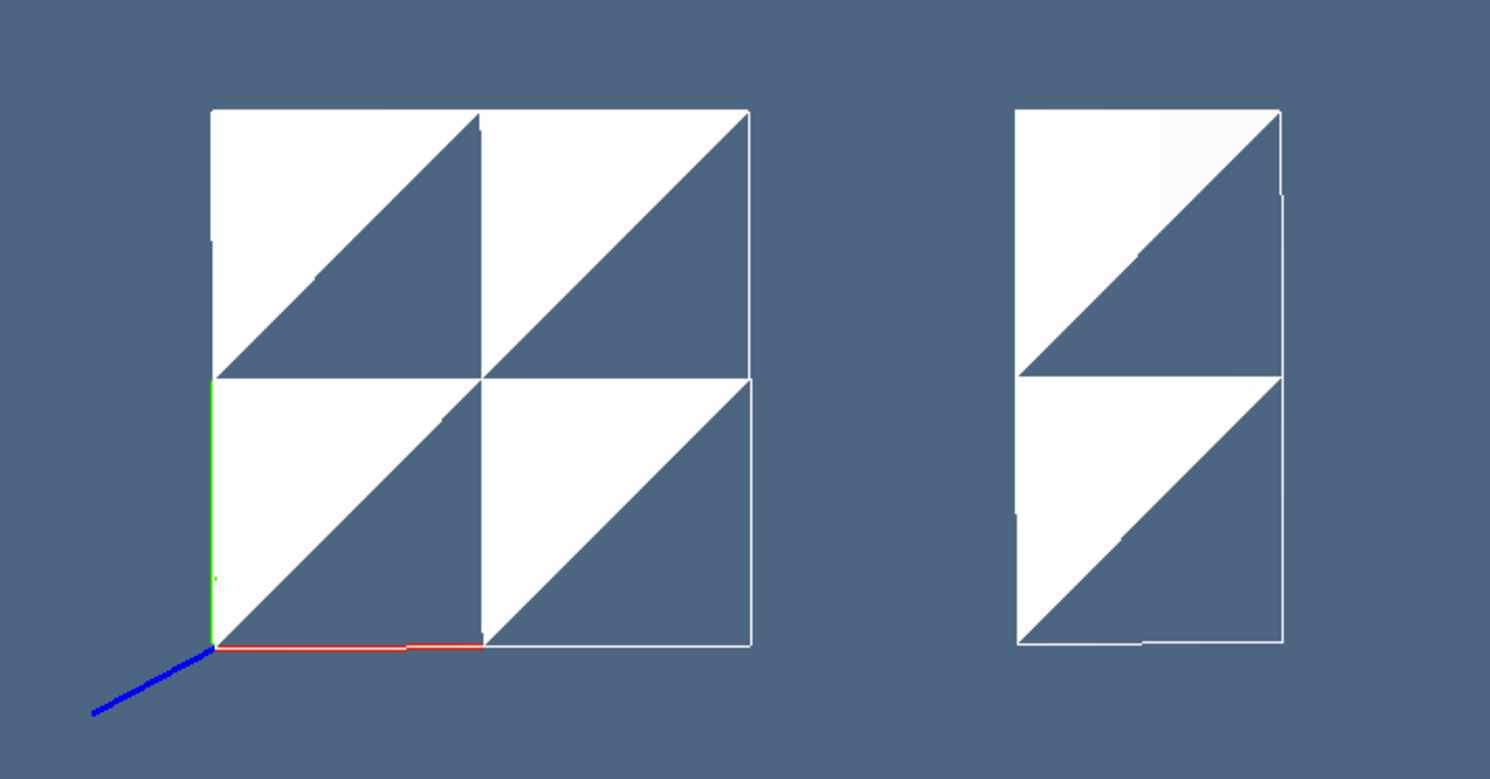
\includegraphics[width=0.405\linewidth]{images/assembly1} 
   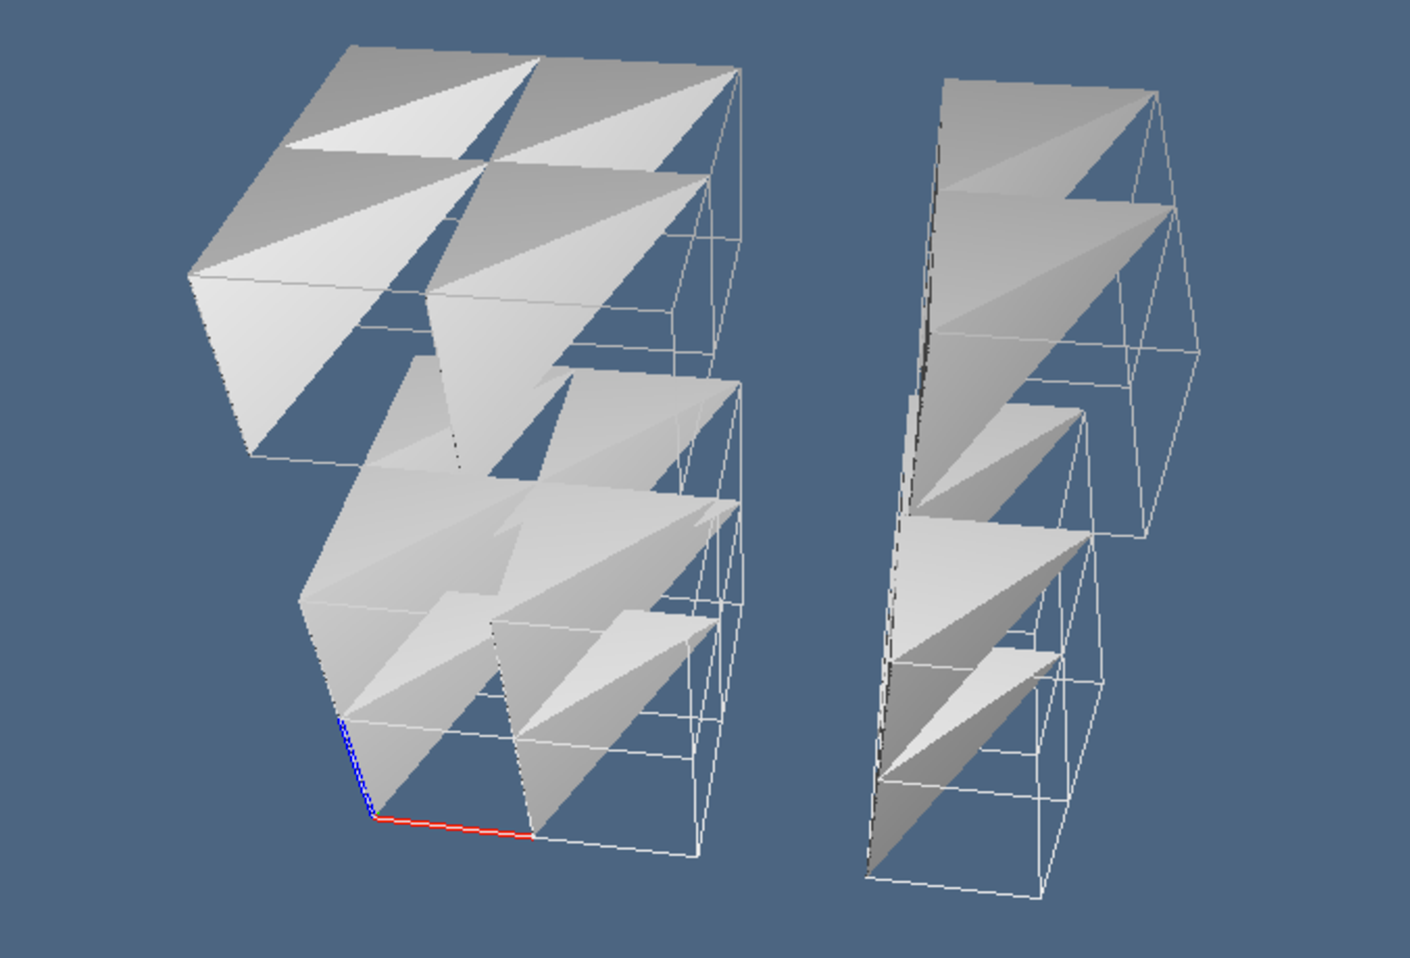
\includegraphics[width=0.315\linewidth]{images/assembly2} 
   \caption{(a) Assemblies of squares and triangles; (b) assembly of cubes and tetrahedra.}
   \label{fig:example}
\end{figure}

%-------------------------------------------------------------------------------
@d Definition of 1-dimensional LAR models 
@{geom_0,topol_0 = [[0.],[1.],[2.],[3.],[4.]],[[0,1],[1,2],[3,4]]
geom_1,topol_1 = [[0.],[1.],[2.]], [[0,1],[1,2]]
mod_0 = (geom_0,topol_0)
mod_1 = (geom_1,topol_1)
@}
%-------------------------------------------------------------------------------

%-------------------------------------------------------------------------------
@d Assembly generation of squares and triangles
@{squares = larModelProduct([mod_0,mod_1])
V,FV = squares
simplices = pivotSimplices(V,FV,d=2)
VIEW(STRUCT([ MKPOL([V,AA(AA(C(SUM)(1)))(simplices),[]]),
              SKEL_1(STRUCT(MKPOLS((V,FV)))) ]))
@}
%-------------------------------------------------------------------------------

%-------------------------------------------------------------------------------
@d Assembly generation  of cubes and tetrahedra 
@{cubes = larModelProduct([squares,mod_0])
V,CV = cubes
simplices = pivotSimplices(V,CV,d=3)
VIEW(STRUCT([ MKPOL([V,AA(AA(C(SUM)(1)))(simplices),[]]),
			  SKEL_1(STRUCT(MKPOLS((V,CV)))) ]))
@}
%-------------------------------------------------------------------------------







\bibliographystyle{amsalpha}
\bibliography{larcc}

\end{document}



\end{document}

